\chapter{驾驶人行为特性对交通流影响}
\section{研究方法}
为了研究驾驶人行为特性对交通流的影响,由于交通流的复杂性,同时由于很难对道路上的驾驶人个体进行逐个的观测与调查,本文使用微观模拟的方法对驾驶人行为特性对交通流影响进行研究。

根据第四章所得出的结果,专业与非专业驾驶人行为的差异主要体现在期望速度和最大减速度这两方面, 因此本章将通过混合不同期望速度和最大减速度参数的驾驶人在典型的道路场景中进行微观模拟仿真从而研究驾驶人行为特性对交通流影响。
\subsection{模拟软件SUMO简介}

根据Krajzewicz等(2006)\cite{Krajzewicz2006}
2000年起,德国航空中心(DLR)的交通研究所(IVF)开始开发微观交通模拟软件。并以开源的形式发布了整个软件包SUMO,作为交通研究中算法和模型的一般测试平台。SUMO为“Simulation of Urban MObility”的缩写,SUMO已被应用于模拟Magdeburg市域和Cologne市域的交通情况,其应用主要关于交通管理和交通预测。

根据Krajzewicz等(2005)\cite{Krajzewicz2005},SUMO的默认值使用了Krauß跟驰模型,Krauß(1998)\cite{Krauss1998}提出了一个微观的空间连续的随机跟驰模型,主要基于安全速度假设:驾驶人为了对前车减速保有一定的安全余量,选择一定的安全速度。模型假设驾驶人的反应时间tau为1s。并且SUMO可以很好的重现密度流量关系图,如\autoref{sumo},图中左边为实测密度流量图,右边为SUMO模拟的密度流量图。

\begin{figure}[!htb]
\begin{center}
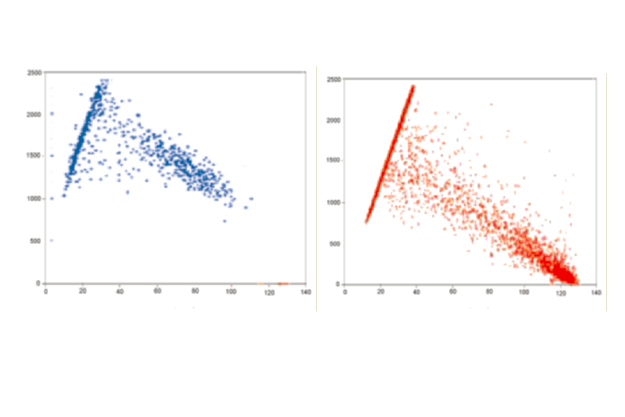
\includegraphics[width=\linewidth]{sumo}
\end{center}
\caption{SUMO模拟密度-流量例图(摘自Krajzewicz等(2005)\cite{Krajzewicz2005})}
\label{sumo}
\end{figure}

Krauß模型给出如下:

\begin{equation}
v_{safe}=v_l(t)+\frac{g(t)-v_l(t)\tau}{\frac{\bar{v}}{b(\bar{v})}+\tau}
\end{equation}

其中:
\begin{displaymath}
{\begin{aligned}
v_l(t)&-t\text{时刻前车速度}\\
g(t)&-t\text{时刻与前车的空间间隔}\\
\tau&-\text{驾驶人的反应时间}\\
b&-\text{减速函数,决定了最大减速度}\\
\end{aligned}}
\end{displaymath}

为了保证车辆不超过其物理加速能力和最大速度,计算$v_{des}(t)$
\begin{equation}
v_{des}(t)=min[v_{safe},v(t)+a_{max},v_{max}]
\end{equation}

最后从期望速度中减去随机项,使得模型变为随机
\begin{equation}
v_{t}(t)=max[0,rand[v_{des}(t)-\epsilon a,v_{des}(t)]]
\end{equation}



\subsection{模拟研究的有效性}

Ossen(2008)\cite{Ossen2008}研究表明,通过Gipps模型构造的人造轨迹数据对Tampère进行参数标定,结果表明即使模型不同,只要有足够的观测,仍可以对驾驶人的跟驰行为得出相似的理解。因此即使不存在完美的跟驰模型,仍可以从实际观测数据对驾驶人行为作出合理推断,同时相似结构的模型可以揭示出相似的驾驶人行为特征。由于Krauß模型与IDM模型的参数结构相似,均考虑了驾驶人的期望速度,最大加速度,最大减速度,从前一章根据IDM模型得出的驾驶人差异性的结论仍可以认为对Krauß模型模型是成立的,因此使用Krauß模型进行模拟是可行的。

% Based on these results it seems justified to conclude that the true car-following behavior of the 
% observed follower can be identified by calibrating an “imperfect” model. 



Kerner\cite{S.Kerner2009}认为,传统的基于基本图的交通流理论不能解释,高速公路交通流的实际观测到的拥堵现象,提出了三相交通流理论。Kerner认为传统跟驰模型不能重现实际观测中的散落的密度-流量基本图。

%这一观点被Helbing认为是错误的,其评论Krauß模型认为由于Krauß模型,不能构成其认为的不连续超车概率因此不能解释F-S和S-J的相位变化。

Schönhof和Helbing\cite{Schoenhof2009}指出传统跟驰模型不能重现实际观测中的散落的密度-流量基本图,是由于未考虑驾驶人驾驶行为的差异性,传统模型的混合驾驶人模拟被证明可以重现实际观测中的散落的密度-流量基本图。


% IDM implementation

\subsection{模拟场景}


如\autoref{scene}中,本文模拟场景设置为600m直线路段,单向3车道,为了增加扰动在路段末端设为2车道.共设置6个线圈检测器,分别在150m处和450m处。

\begin{figure}[!htb]
\begin{center}
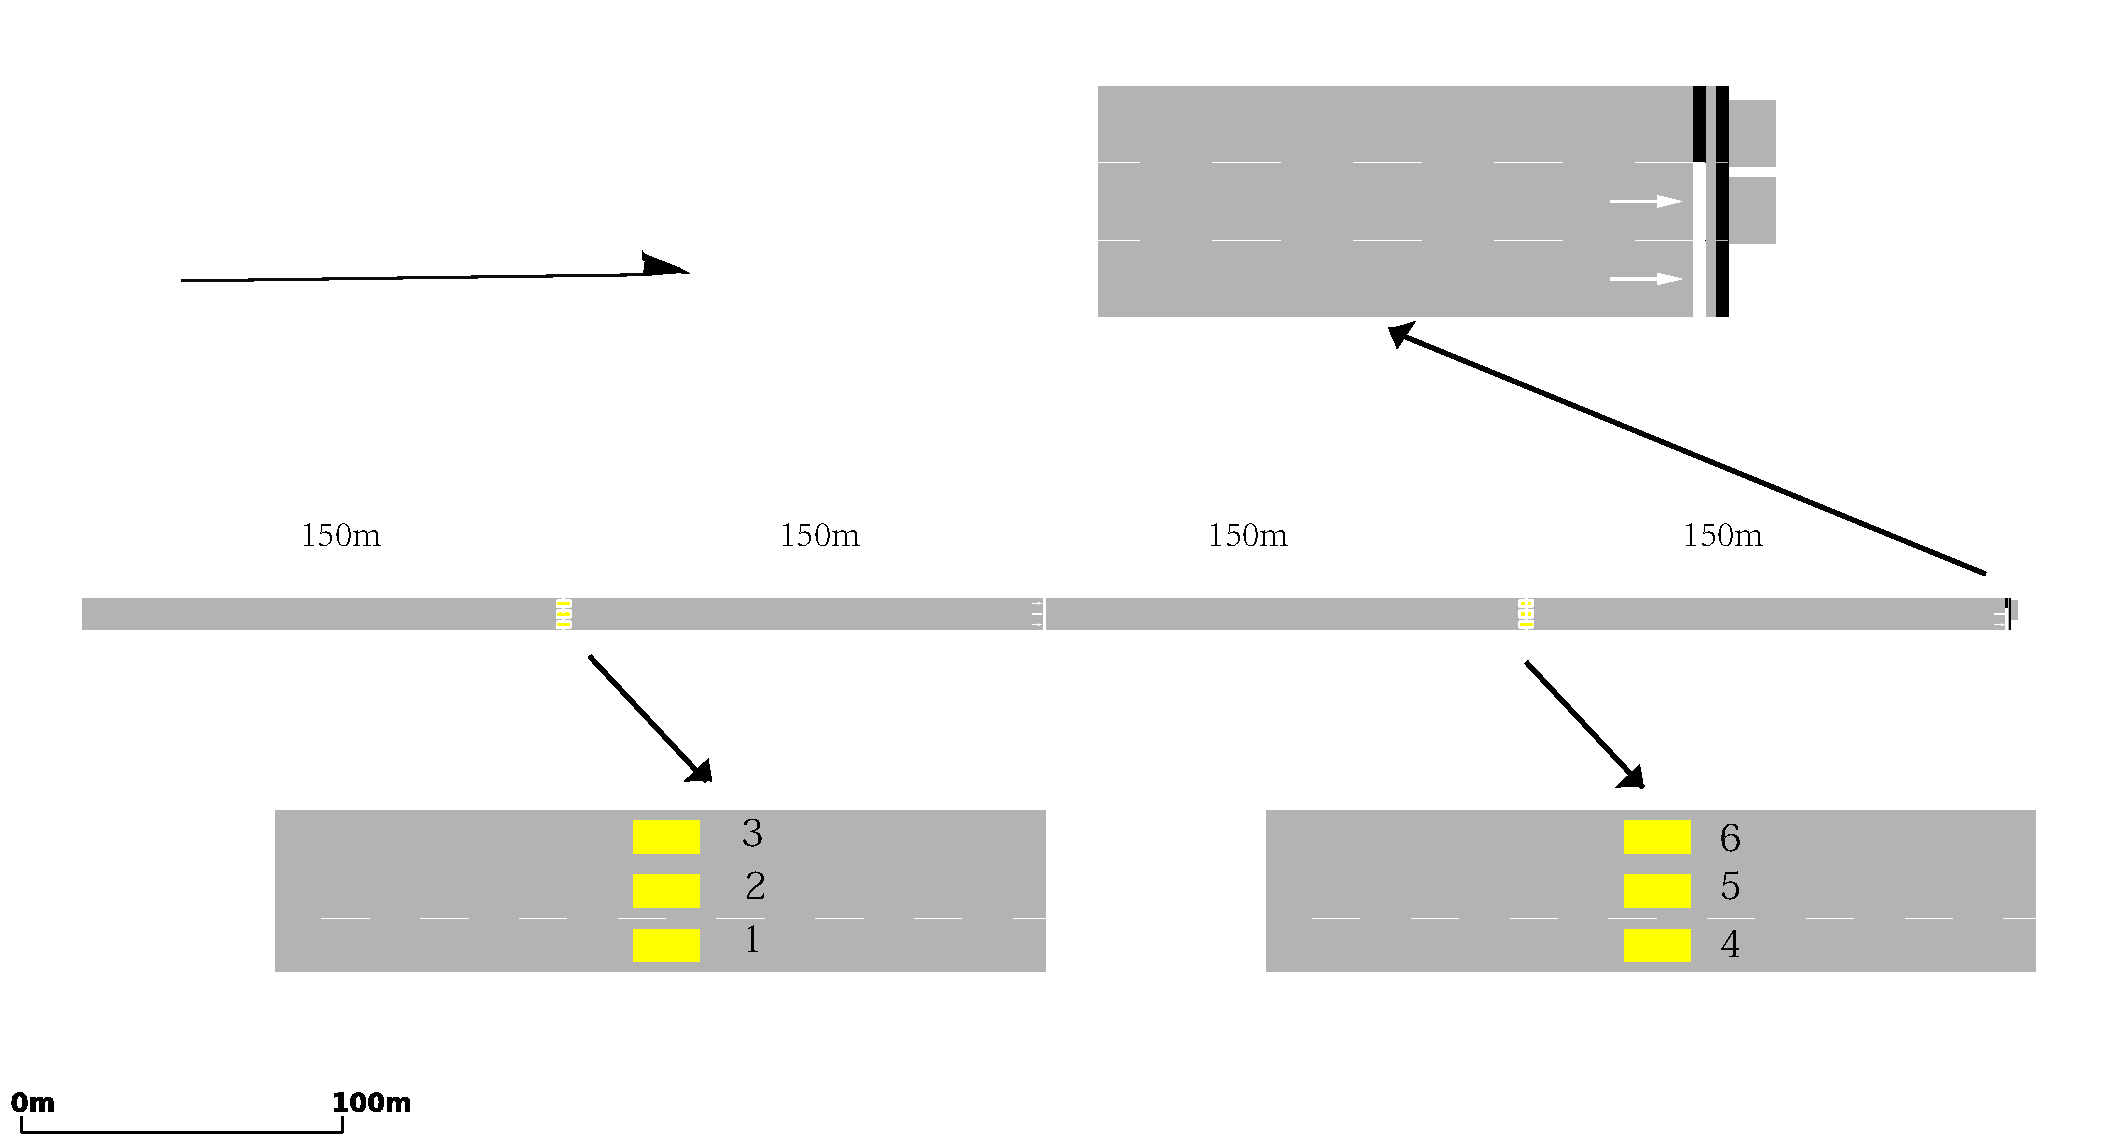
\includegraphics[width=\linewidth]{scene}
\end{center}
\caption{模拟场景图}
\label{scene}
\end{figure}

模拟中的输入的交通流量设为三条车道均等,设置0-1200s,流率为600辆/小时,1200-2400s,流率为1800辆/小时,2400-4800s,流率为600辆/小时,如\autoref{input-demand}

\begin{figure}[!htb]
\begin{center}
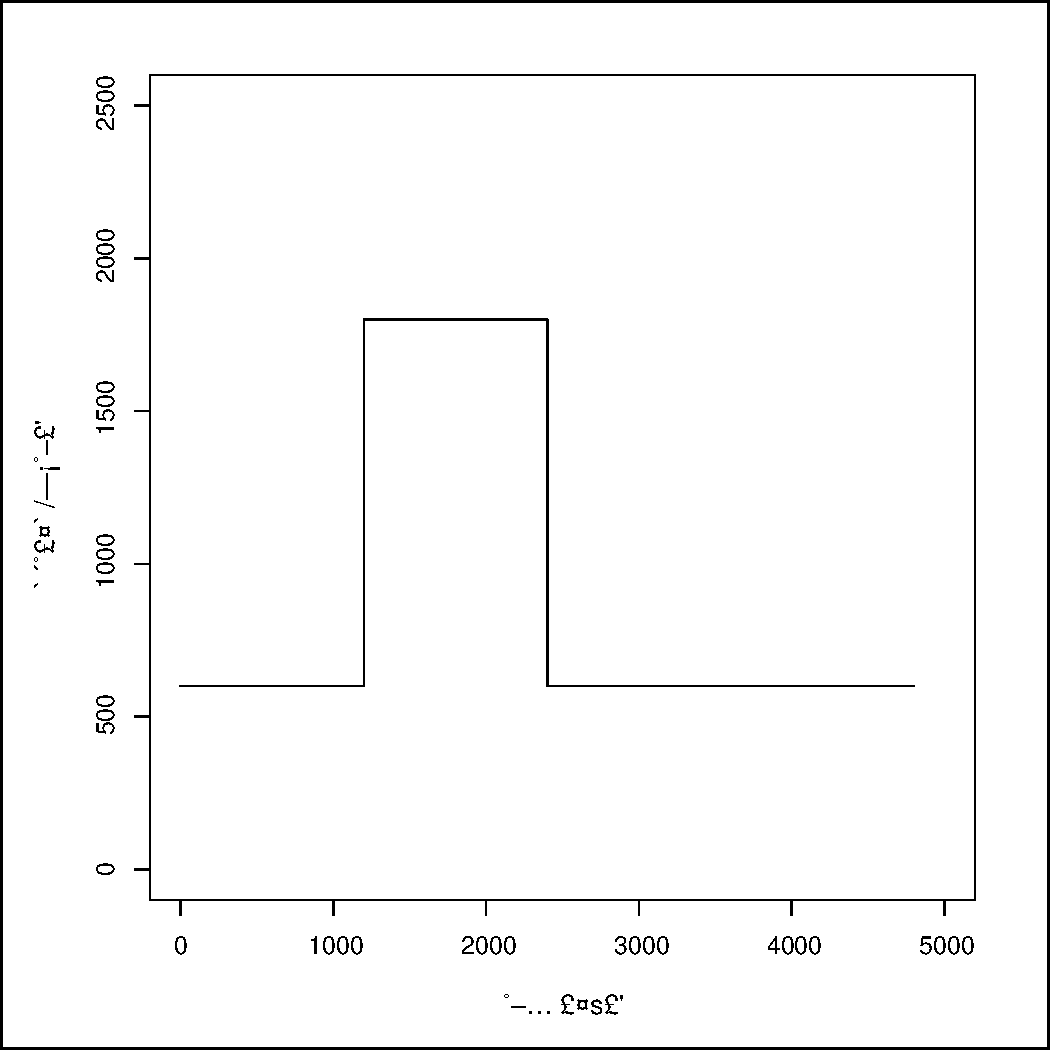
\includegraphics[width=0.3\linewidth]{input-demand}
\end{center}
\caption{交通需求随时间变化图}
\label{input-demand}
\end{figure}

为了研究驾驶人行为特性对交通流的影响,结合第四章所得结论。主要考察三种效应的影响,一为驾驶人期望车速对交通流的影响,二是驾驶人最大减速度对交通流的影响,三为两者混合效应(专业与非专业驾驶人混合)的影响。



针对三种效应,对每一种效应分别选择A、B两种驾驶人,以不同数值赋予所研究效应的对应参数,分别如\autoref{speed-factor},\autoref{decel-factor}和\autoref{combined-factor}。表中A、B型驾驶人的模型参数选择了第四章跟驰模型参数标定结果的平均值。
以全部A类型驾驶人,1:3,1:1和3:1的比例混合和全部B类型驾驶人分别进行模拟,也就是说B类型的驾驶人从0\%到25\%,50\%,75\%增加到100\%,由于在驾驶人混合中,车辆的出发顺序随机,在驾驶人混合中以不同随机种子数模拟10次。

尽管Krauss(1998)\cite{Krauss1998}指出,Krauß模型之所以能够模拟实际观测中出现的交通流相位变化是由于其随机项导致的,但是其模拟的速度轨迹往往很不符合实际情况,并且其模型中随机项对交通流的影响没有确定性的结论,为了减少其他影响因素本文模拟中未使用随机项,而驾驶人的反应时间tau设置为1s。

\begin{table}[htb] 
  \begin{minipage}[b]{0.25\linewidth} 
  \centering
  \caption{期望速度效应的模型参数}
    \begin{tabular}{rrr}
    \addlinespace
    \toprule
    驾驶人类型    & A     & B \\
    \midrule
    最大加速度 & 0.62  & 0.62 \\
    最大减速度 & 2.33  & 2.33 \\
    期望速度  & 6.48  & 8.09 \\
    \bottomrule
    \end{tabular}%
  \label{speed-factor}%
  \end{minipage}% 
\hspace{0.08\linewidth}
  \begin{minipage}[b]{0.25\linewidth} 
  \centering
  \caption{最大减速度效应的模型参数}
    \begin{tabular}{rrr}
    \addlinespace
    \toprule
    驾驶人类型    & A     & B \\
    \midrule
    最大加速度 & 0.62  & 0.62 \\
    最大减速度 & 2.33  & 4.29 \\
    期望速度  & 8.09  & 8.09 \\
    \bottomrule
    \end{tabular}%
  \label{decel-factor}%
  \end{minipage}
\hspace{0.08\linewidth}
  \begin{minipage}[b]{0.25\linewidth} 
  \centering
  \caption{混合效应的模型参数}
    \begin{tabular}{rrr}
    \addlinespace
    \toprule
    驾驶人类型    & A     & B \\
    \midrule
    最大加速度 & 0.62  & 0.62 \\
    最大减速度 & 2.33  & 4.29 \\
    期望速度  & 8.09  & 6.48 \\
    \bottomrule
    \end{tabular}%
  \label{combined-factor}%
  \end{minipage} 
\end{table}






\subsection{评价指标}
本文主要从效率性和安全性两个角度评价对交通流的影响作用。

效率性方面,主要从模拟所需要的总时间、速度流量基本图、密度流量基本图来分析交通流效率性的影响。



安全性方面,通过SUMO的轨迹输出计算TTC倒数值,\refsec{ttc}给出了TTC及TTC倒数的定义。其中仅考虑前车速度较小的情况,也就是TTC值为负的情况,符号仅代表速度差的方向,其大小以绝对值进行比较,绝对值越大代表越危险。评价中以TTC倒数与流量的关系和模拟时间内的TTC倒数的时间平均值来评价安全性。


\section{三相交通流理论简介}
下文中由于涉及到三相交通流理论的概念,此处对三相交通流理论作简要介绍。

Kerner和Rehborn(1996,1996a,1997)\cite{Kerner1996,Kerner1996a,Kerner1997},Kerner(1998)\cite{Kerner1998}通过对德国A5高速公路的观测,发现了一系列高速公路交通流中的拥堵形成与消散的特殊现象。基于这些经验性的观测,Kerner(2004)\cite{Kerner2004}提出了三相交通流理论。

\subsection{三个相位}
在三相交通流的理论框架下,共分三个交通流的相位,分别为自由流相位F、同步流相位S和宽运动阻塞流相位J。

其中自由流为速度较高,各车道车速无显著相同趋势的相位。表现为密度流量图上,流量随着密度线性增加的区域。除了自由流以外的相位为拥挤流,拥挤流有分为同步流相位和宽运动阻塞流相位。

宽运动阻塞流相位的特征为,车速很低有时降为零,阻塞的下游前端保持一定速度向上游传播。

拥挤流其他的状态被归为同步流,同步流速度显著不为零,且下游前端并不保持一定的速度,往往位于瓶颈处。同步流的名称得自于其车辆间和车道间的速度同步效应。



\subsection{相位转换}
为了解释相位变化,根据Kerner(2009)\cite{S.Kerner2009},主要存在三种效应Speed Adaptation,Over-Acceleration和Over-Deceleration,它们之间的相互竞争导致了交通流的相位变化。

Speed Adaptation效应,指的是当车辆无法超越前方的慢车时,其车速与前车车速趋于相同的效应,speed adaptation效应解释了当前后车车速相同时,跟驰距离在一定的范围内变动。Speed Adaptation效应的速度跟驰距离示意图如\autoref{speed_adapt}

Over-Acceleration效应,指的是在前车速度较慢的情况下,驾驶人寻找机会超车的行为。

\begin{figure}[htbp]
\begin{minipage}[t]{0.48\linewidth}
\centering
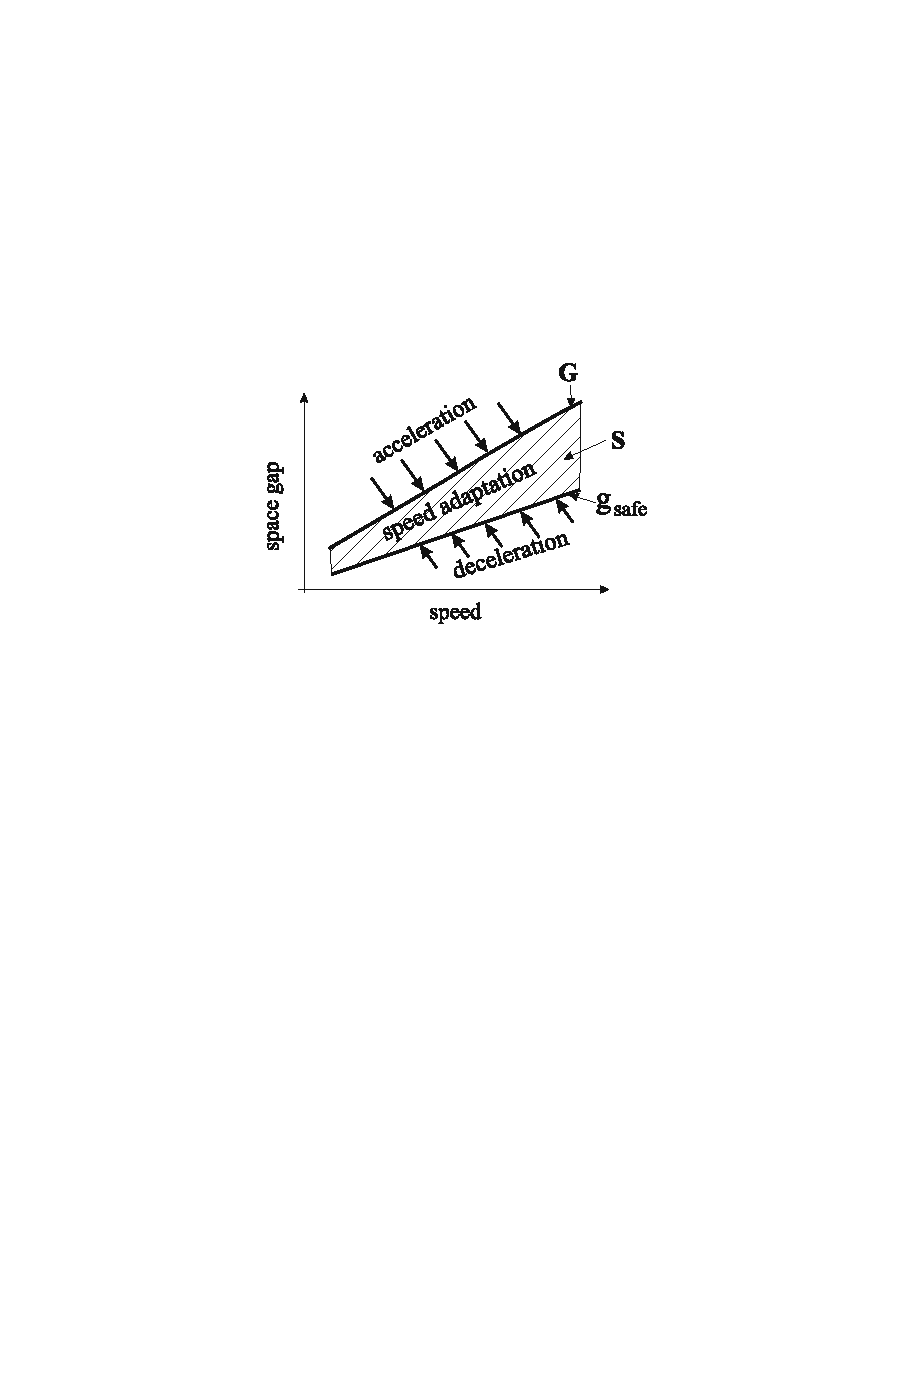
\includegraphics[width=\textwidth]{speed_adapt}
\caption{Speed Adaptation效应的速度跟驰距离示意图\cite{S.Kerner2009}}
\label{speed_adapt}
\end{minipage}%
\hspace*{0.04\linewidth}
\begin{minipage}[t]{0.48\linewidth}
\centering
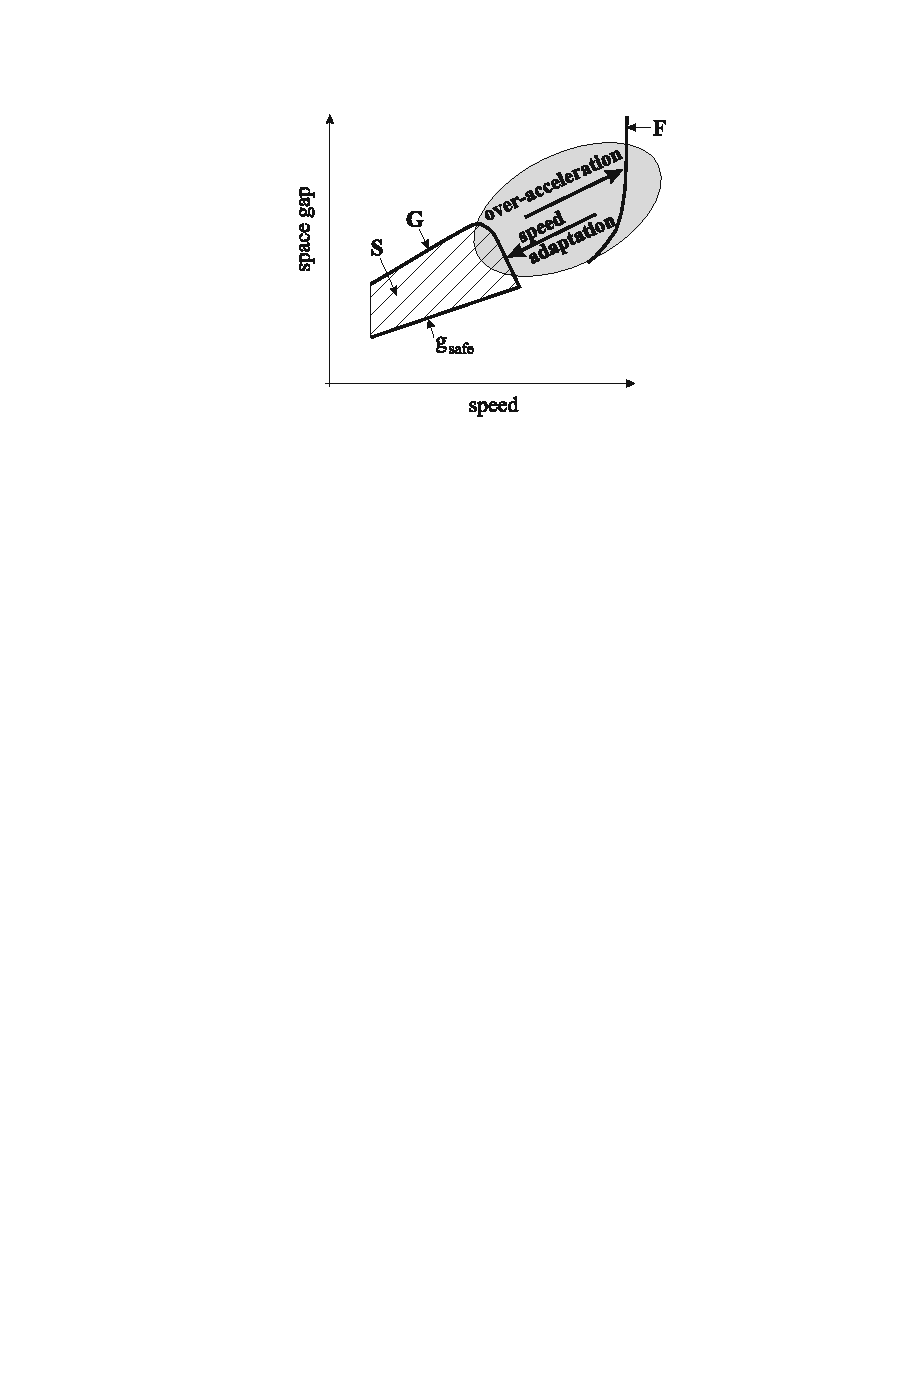
\includegraphics[width=\textwidth]{fscompete}
\caption{Speed Adaptation效应和Over-Acceleration效应竞争示意图\cite{S.Kerner2009}}
\label{fscompete}
\end{minipage}
\end{figure}

Over-Deceleration效应,指的是当前车忽然减速的情况下,驾驶人有一个延后时间才开始减速,如果驾驶人过度减速则会使得车速慢于前车,当这种扰动不断向上游传递,速度的降低幅度会逐渐累积而增大。

Kerner将相位的转换解释为这三种效应的两两竞争,自由流F和同步流S的相互转换为Speed Adaptation效应和Over-Acceleration效应相互竞争的结果,其示意图如\autoref{fscompete},同步流S和宽运动阻塞流J的相互转换为Speed Adaptation效应和Over-Deceleration效应相互竞争的结果。

\subsection{无数个通行能力和J线的含义}

根据实际观测中的密度流量图,三相交通流理论认为不存在唯一的通行能力,而是在一定密度范围内自由流均有概率发生F到S的相位变化,因此提出了无数个通行能力的概念。其示意图如\autoref{infi_capacity}。

三相交通流理论中的J线为密度流量图上代表宽运动阻塞的稳定传播的直线,其斜率由宽运动阻塞流前端的平均速度决定,J线将同步流区域划分为两块,J线以上为微妙稳定的同步流状态,而J线以下为稳定的同步流状态。微妙稳定的同步流状态指S相位到J相位 的转换可以自行发生。J线的示意图如\autoref{jline}。

\begin{figure}[htbp]
\begin{minipage}[t]{0.48\linewidth}
\centering
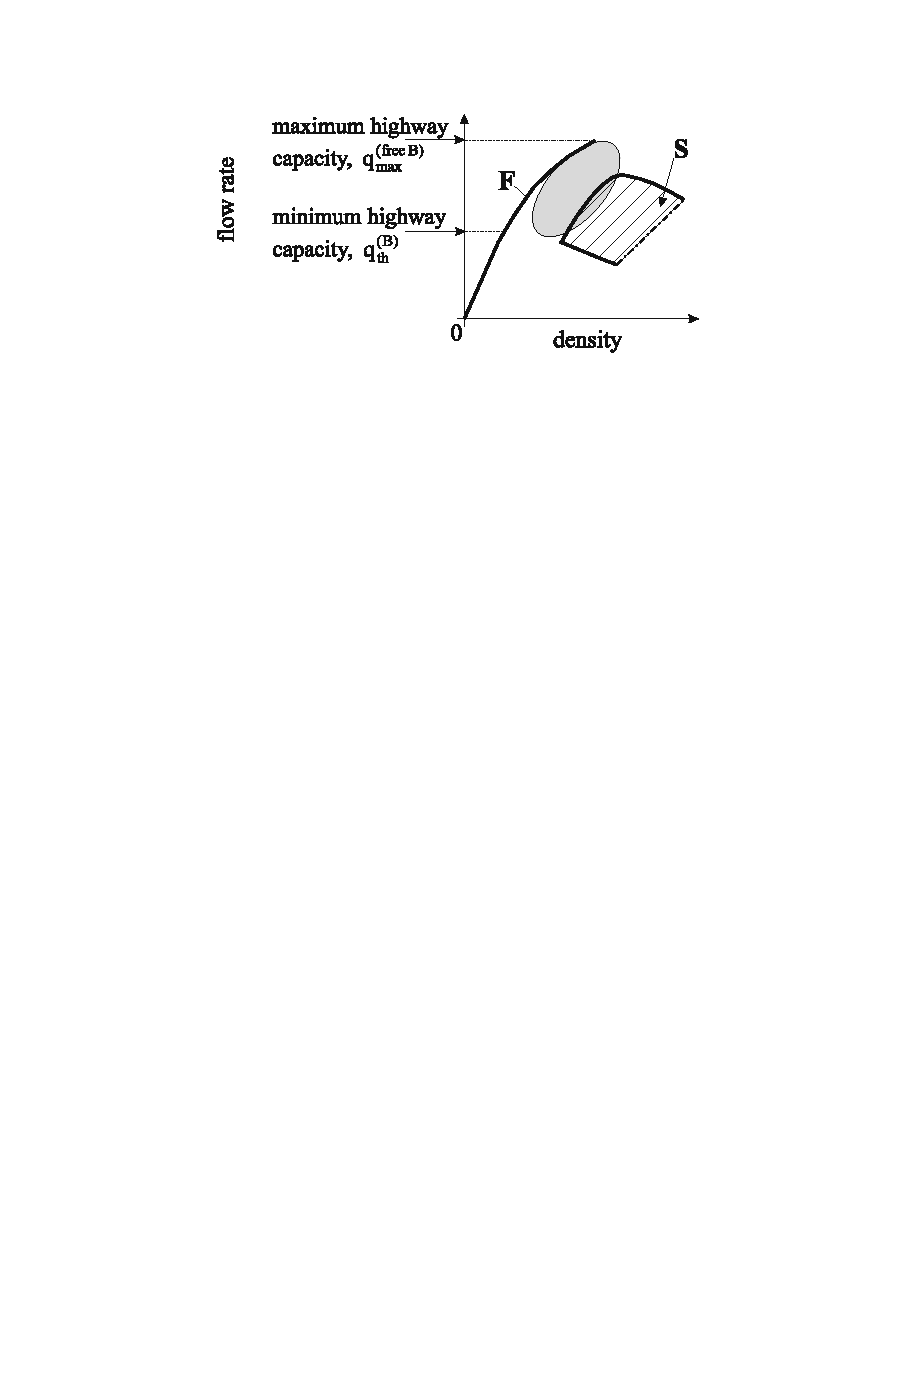
\includegraphics[width=\textwidth]{infi_capacity}
\caption{无数个通行能力的示意图\cite{S.Kerner2009}}
\label{infi_capacity}
\end{minipage}%
\hspace*{0.04\linewidth}
\begin{minipage}[t]{0.48\linewidth}
\centering
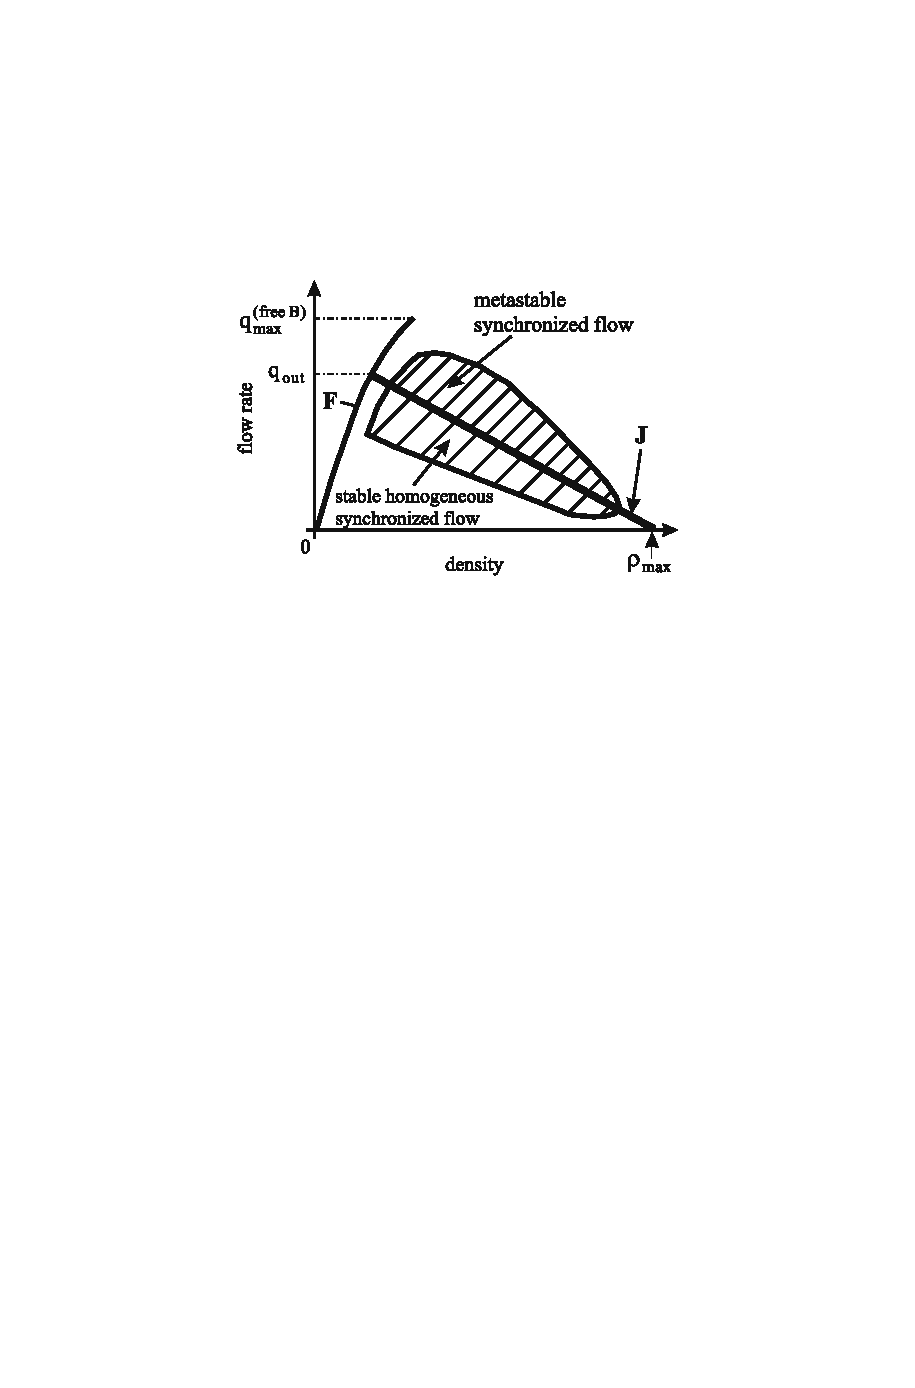
\includegraphics[width=\textwidth]{jline}
\caption{J线示意图\cite{S.Kerner2009}}
\label{jline}
\end{minipage}
\end{figure}


% \section{驾驶人行为特性对交通流效率性的影响}

% \subsection{期望速度影响因素}
% 根据\autoref{speed-factor}的驾驶人参数进行混合模拟,得到:

% \begin{figure}[!htb]
% \begin{center}
% 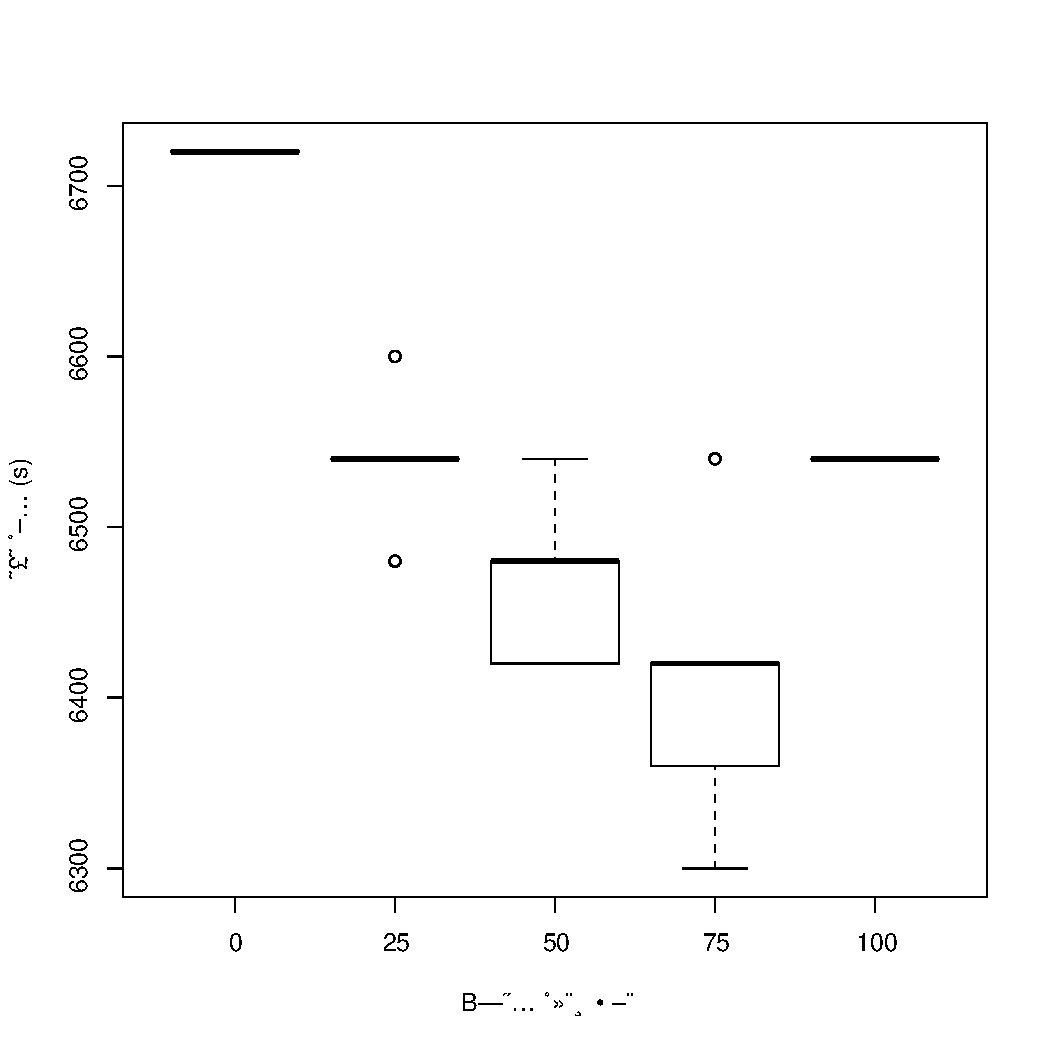
\includegraphics[width=0.5\linewidth]{factor1_box_ttime}
% \caption{期望速度影响下模拟用时箱图}
% \label{factor1_box_ttime}
% \end{center}
% \end{figure}

% \autoref{factor1_box_ttime}给出了,期望速度影响下模拟总用时的变化,随着\autoref{speed-factor}中期望速度较大的B型驾驶人的增加,模拟所用时间呈现下降的趋势。对于单纯类型的驾驶人组合,期望速度由6.48m/s(23.3km/h)增加8.09m/s(30.6km/h),增加24.8\%,模拟用时从6720s下降到6540s,降低了3\%。


% \begin{figure}[!htb]%
% \centering
% \subfloat[][]{
% \label{factor1_vq_per0}%
% 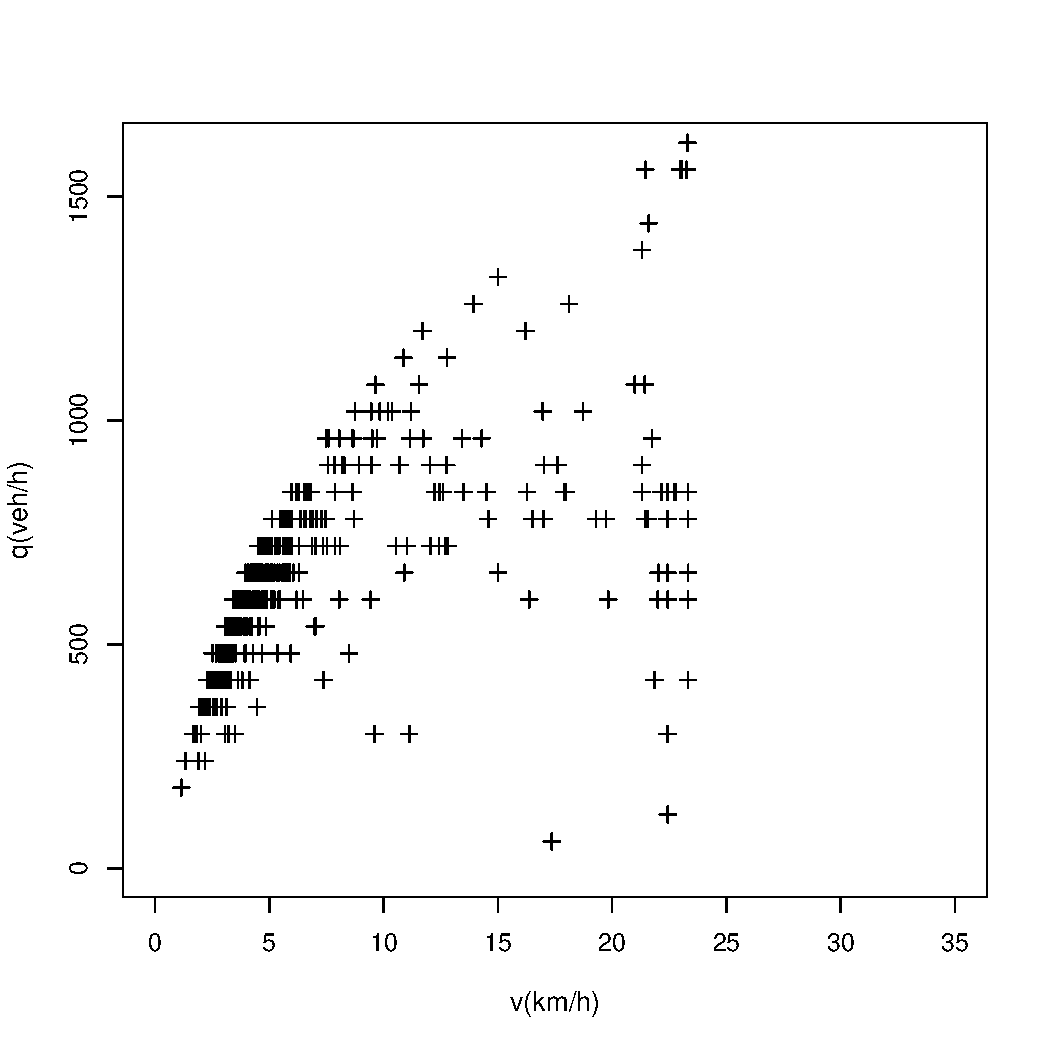
\includegraphics[width=0.25\linewidth]{factor1_vq_per0}
% }%
% \subfloat[][]{%
% \label{factor1_vq_per25}%
% 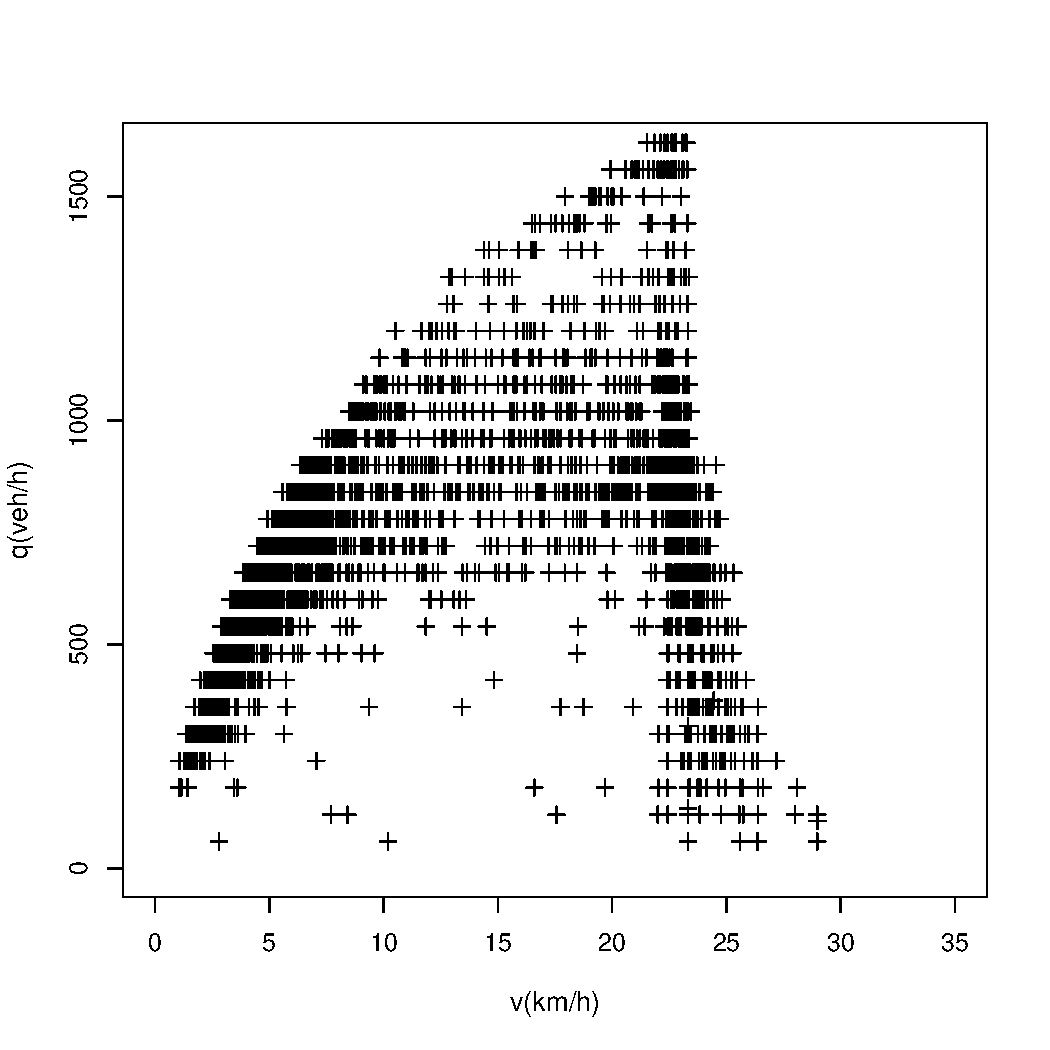
\includegraphics[width=0.25\linewidth]{factor1_vq_per25}}
% \subfloat[][]{%
% \label{factor1_vq_per50}%
% 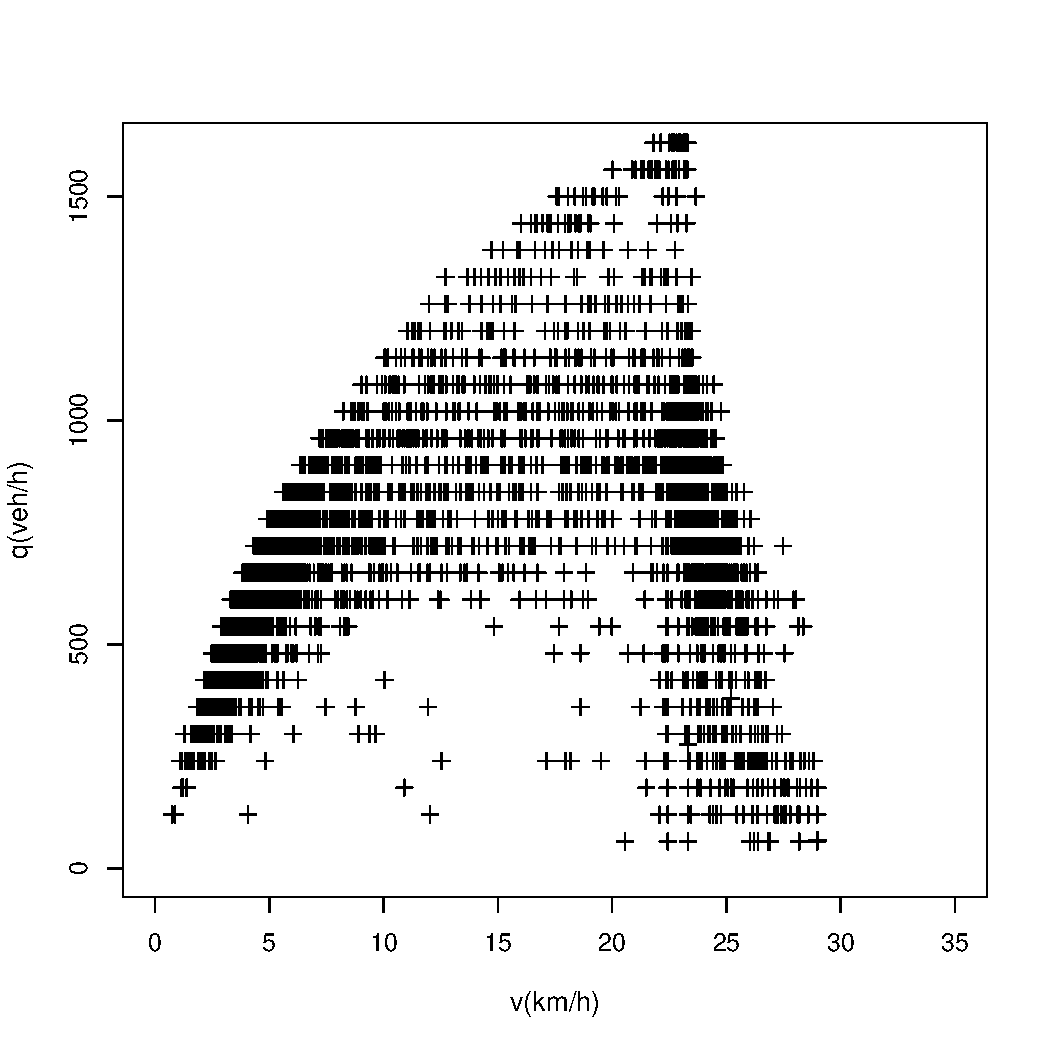
\includegraphics[width=0.25\linewidth]{factor1_vq_per50}}\\%
% \subfloat[][]{%
% \label{factor1_vq_per75}%
% 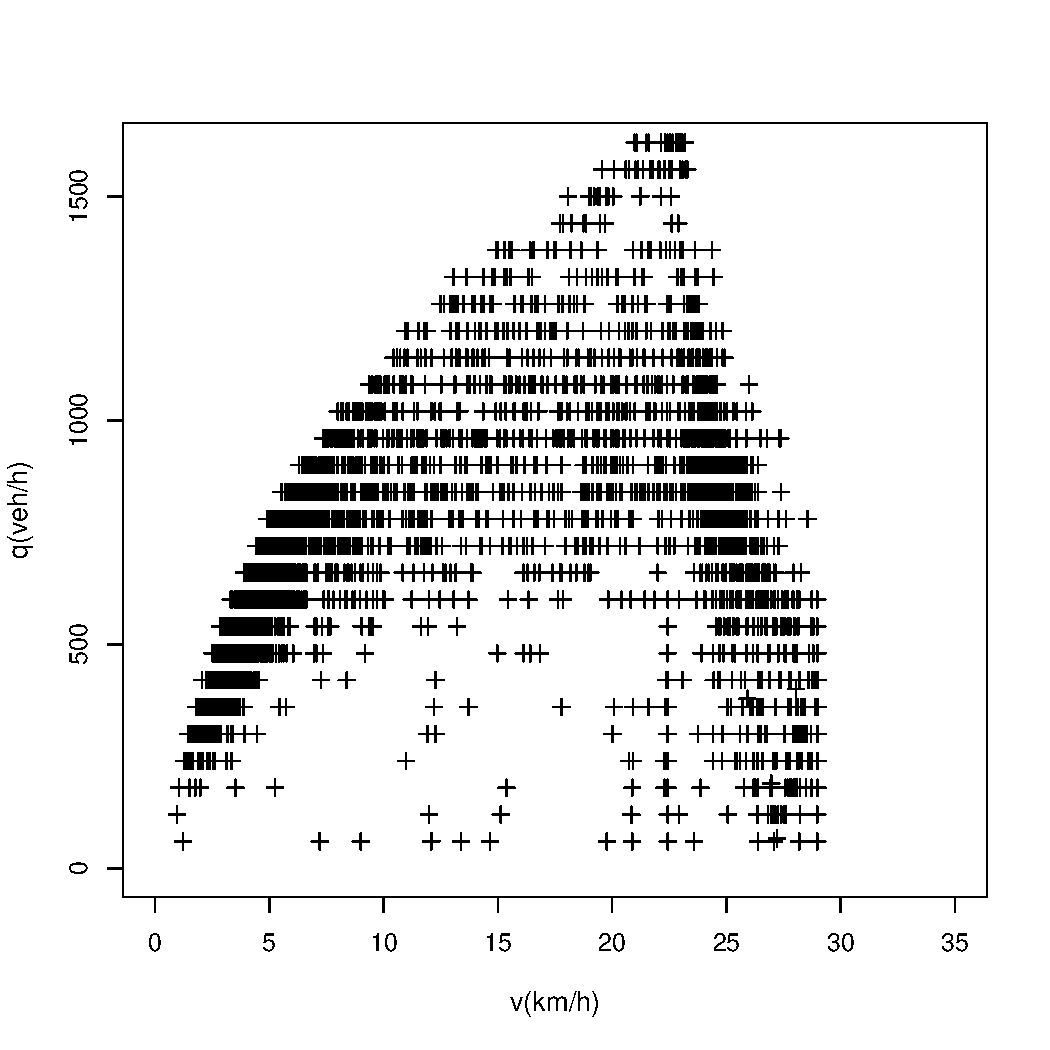
\includegraphics[width=0.25\linewidth]{factor1_vq_per75}}%
% \subfloat[][]{%
% \label{factor1_vq_per100}%
% 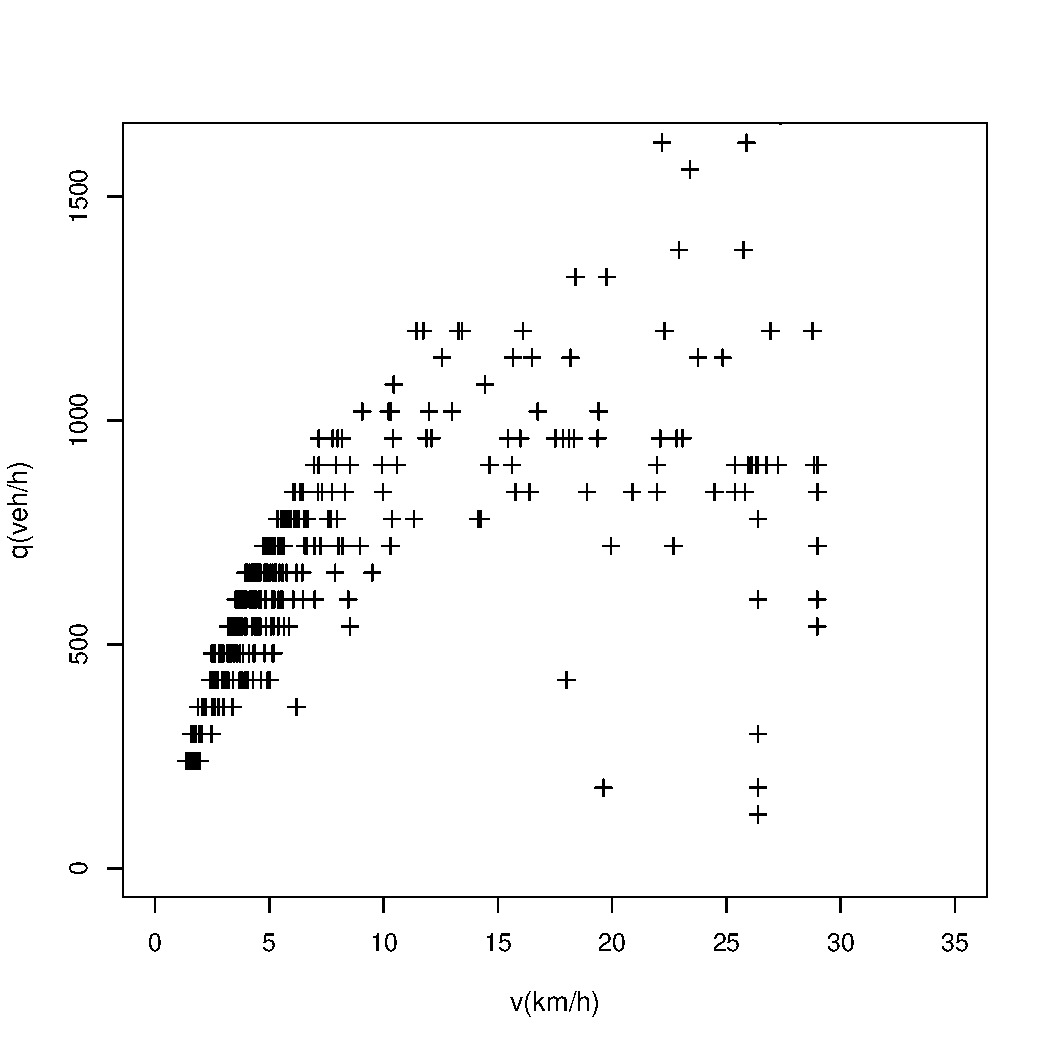
\includegraphics[width=0.25\linewidth]{factor1_vq_per100}}
% \caption[A set of four sub-floats.]{期望速度影响下速度流量关系图
% \subref{factor1_vq_per0}
% \subref{factor1_vq_per25} 
% \subref{factor1_vq_per50}
% \subref{factor1_vq_per75}
% \subref{factor1_vq_per100}分别表示\autoref{speed-factor}中的B型驾驶人的百分比分别为0\%,25\%,50\%,75\%,100\%}%
% \label{factor1_vq}%
% \end{figure}

% 由\autoref{factor1_vq}可以看出,期望速度主要对速度-流量关系图中的形状有影响,对最大通行能力和最大通行能力所对应的最佳车速基本没有影响,图中可以看出最大通行能力约为1600veh/h,最佳速度大约均在22km/h。期望速度对速度-流量关系图中的形状的影响主要体现在,最佳车速的右侧主要为自由流的阶段。由于两组的期望速度均超过了最佳车速,因此不能排除当期望速度低于最佳车速时可能会对最大通行能力产生影响。



% \begin{figure}[!htb]%
% \centering
% \subfloat[][]{
% \label{factor1_kq_per0}%
% 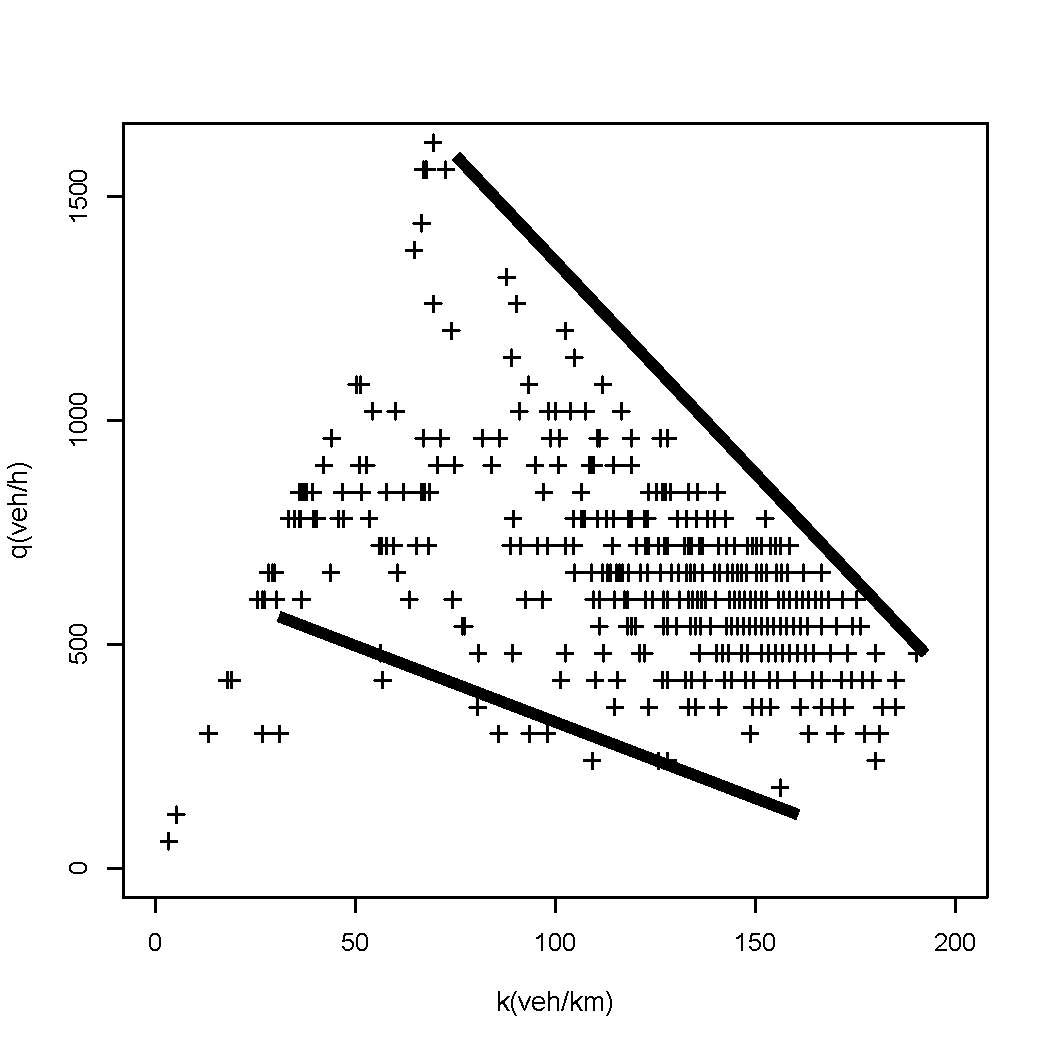
\includegraphics[width=0.25\linewidth]{factor1_kq_per0}
% }%
% \subfloat[][]{%
% \label{factor1_kq_per25}%
% 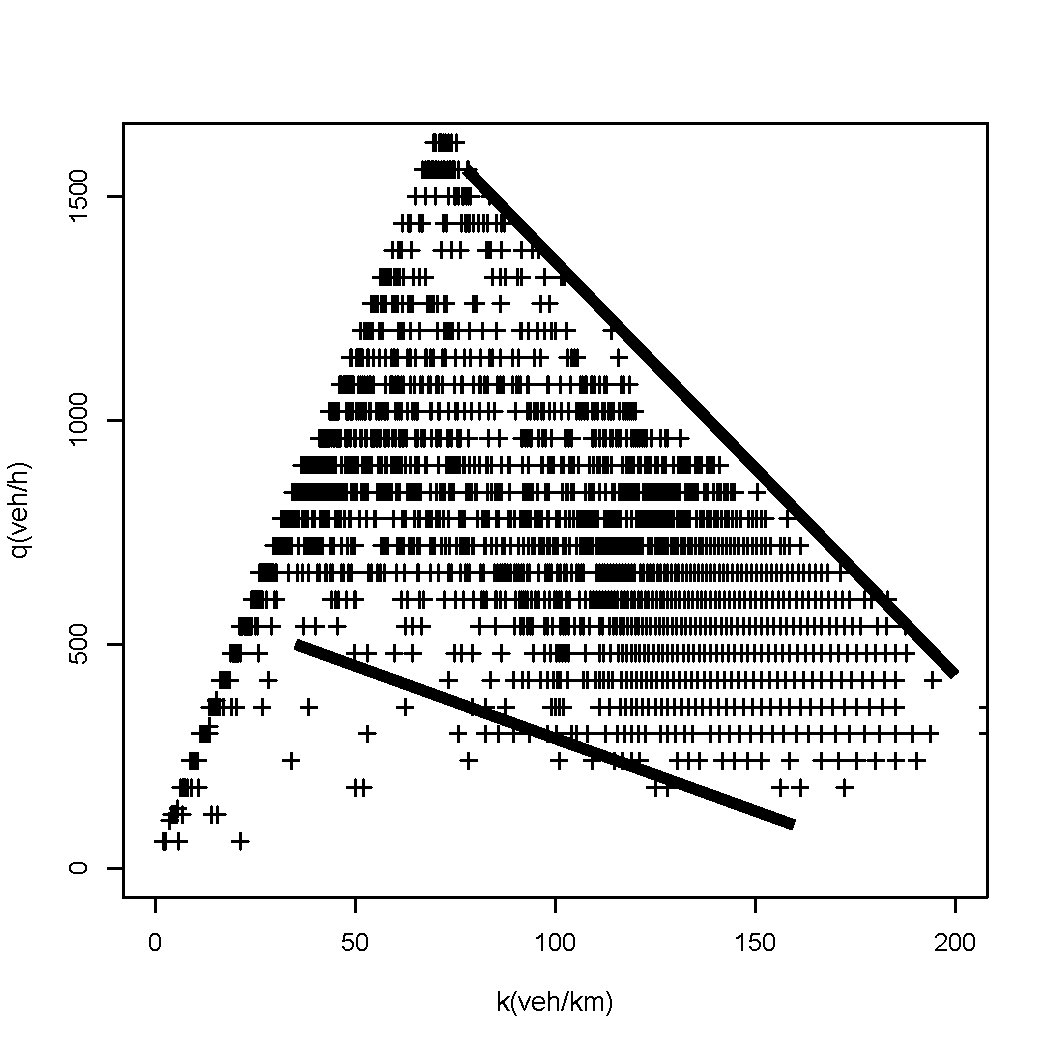
\includegraphics[width=0.25\linewidth]{factor1_kq_per25}}
% \subfloat[][]{%
% \label{factor1_kq_per50}%
% 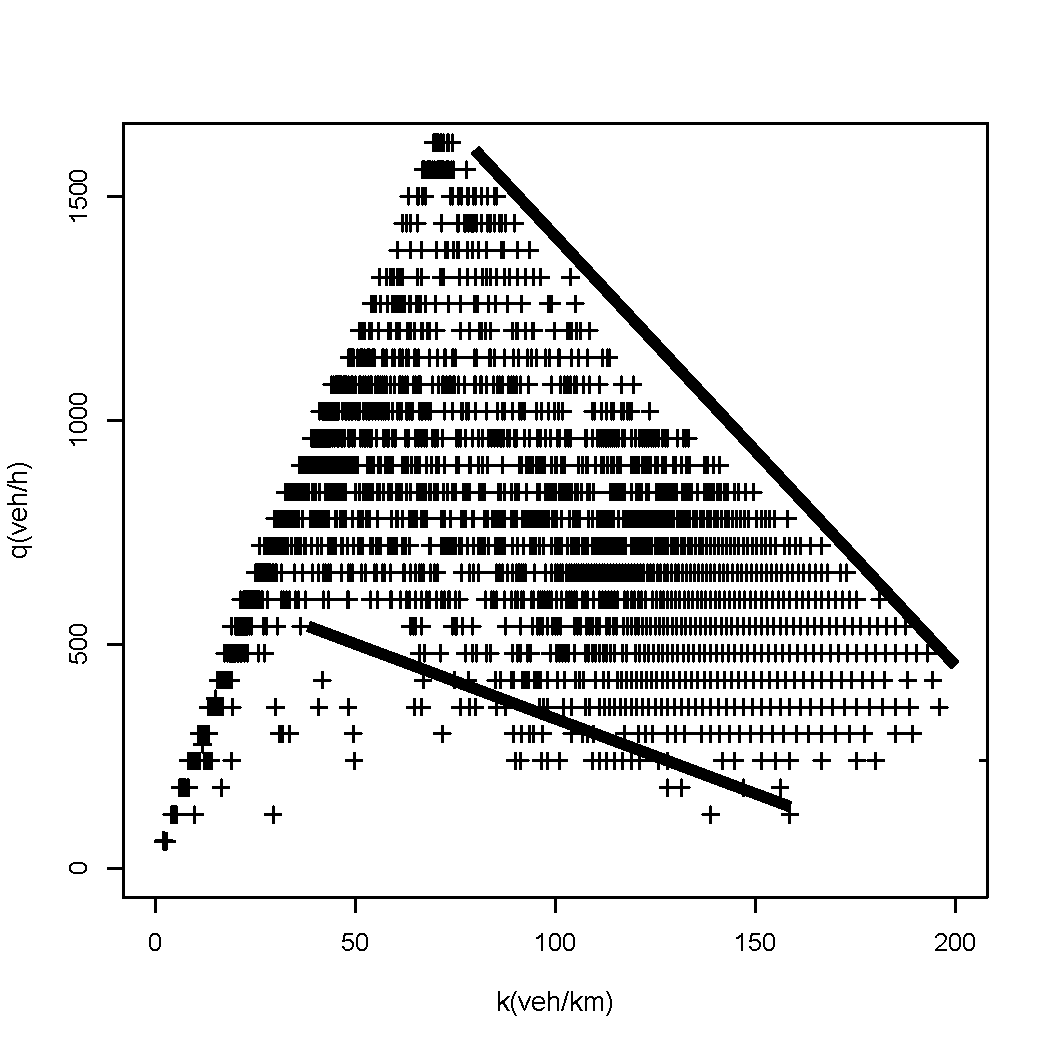
\includegraphics[width=0.25\linewidth]{factor1_kq_per50}}\\%
% \subfloat[][]{%
% \label{factor1_kq_per75}%
% 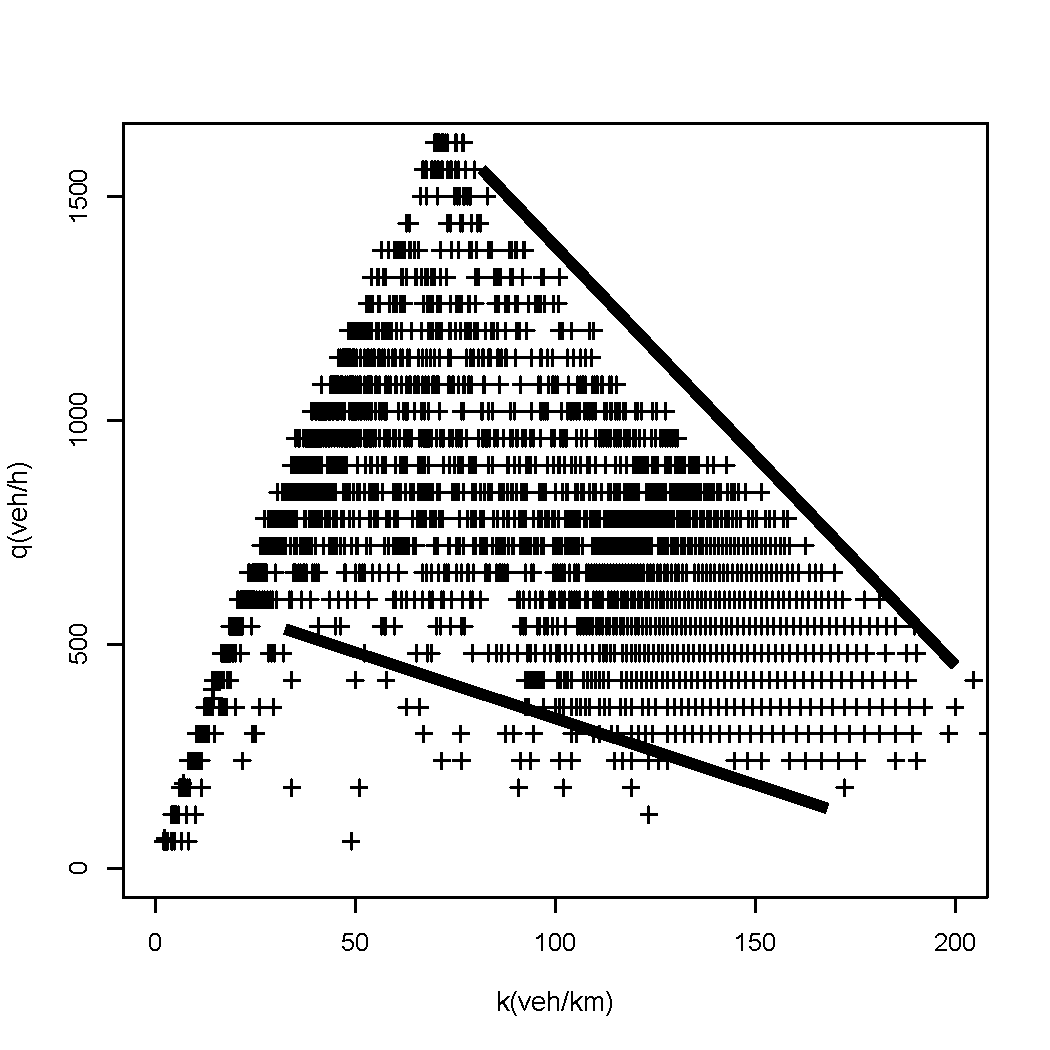
\includegraphics[width=0.25\linewidth]{factor1_kq_per75}}%
% \subfloat[][]{%
% \label{factor1_kq_per100}%
% 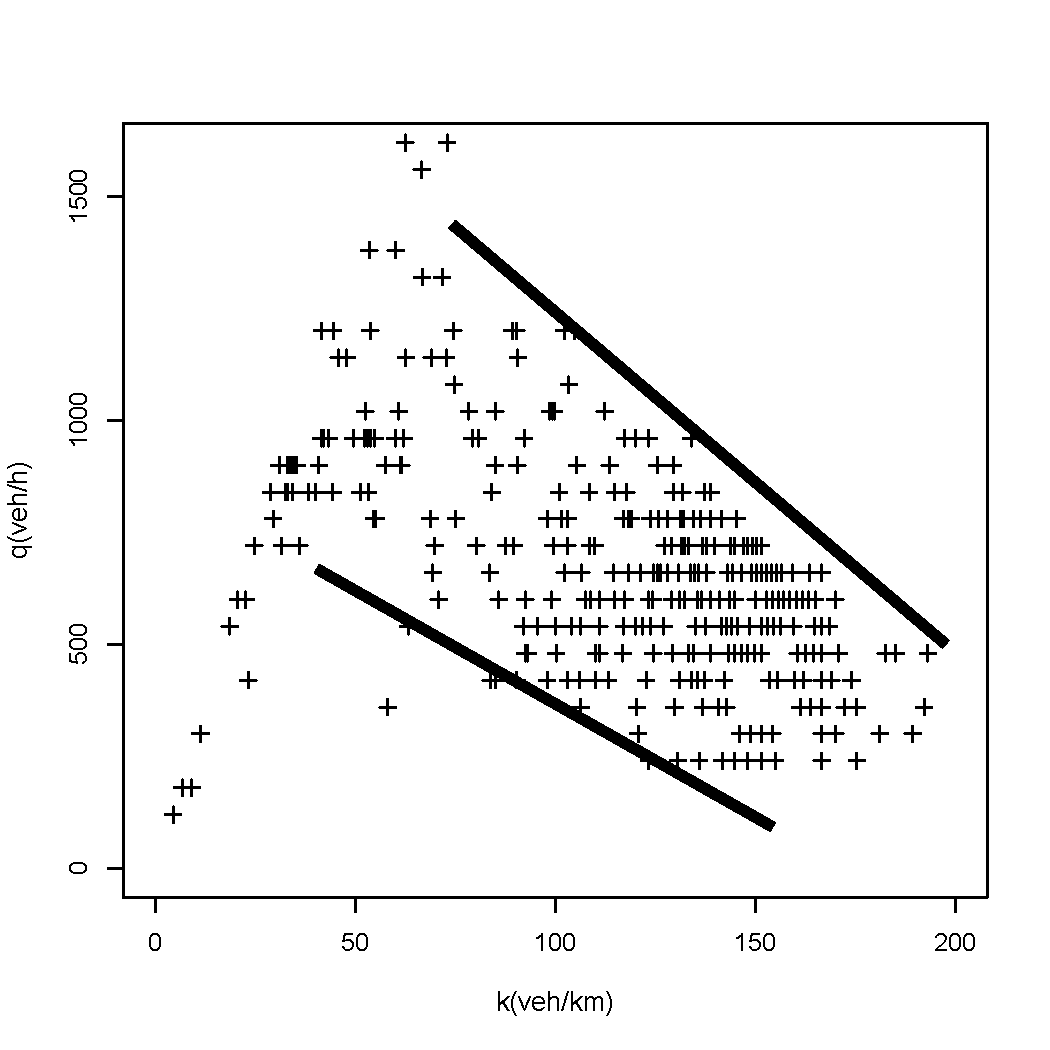
\includegraphics[width=0.25\linewidth]{factor1_kq_per100}}
% \caption[A set of four sub-floats.]{期望速度影响下的密度流量关系图
% \subref{factor1_kq_per0}
% \subref{factor1_kq_per25} 
% \subref{factor1_kq_per50}
% \subref{factor1_kq_per75}
% \subref{factor1_kq_per100}分别表示\autoref{speed-factor}中的B型驾驶人的百分比分别为0\%,25\%,50\%,75\%,100\%}%
% \label{factor1_kq}%
% \end{figure}

% 由\autoref{factor1_kq},期望速度对最佳密度基本没有影响。根据Kerner的三相交通流理论,道路介于最大和最小通行能力之间具有无数个通行能力,\autoref{factor1_kq}中e的最小通行能力稍大于其他的情况,这似乎表明最小通行能力受到最低期望车速的影响。

%由于低期望车速的驾驶人的存在,???根据三相交通流中Speed adaptation效用的作用,低速车辆的阻碍造成最低通行能力的下降是可以理解的。

% \subsection{最大减速度影响因素}

% \begin{figure}[!htb]
% \begin{center}
% 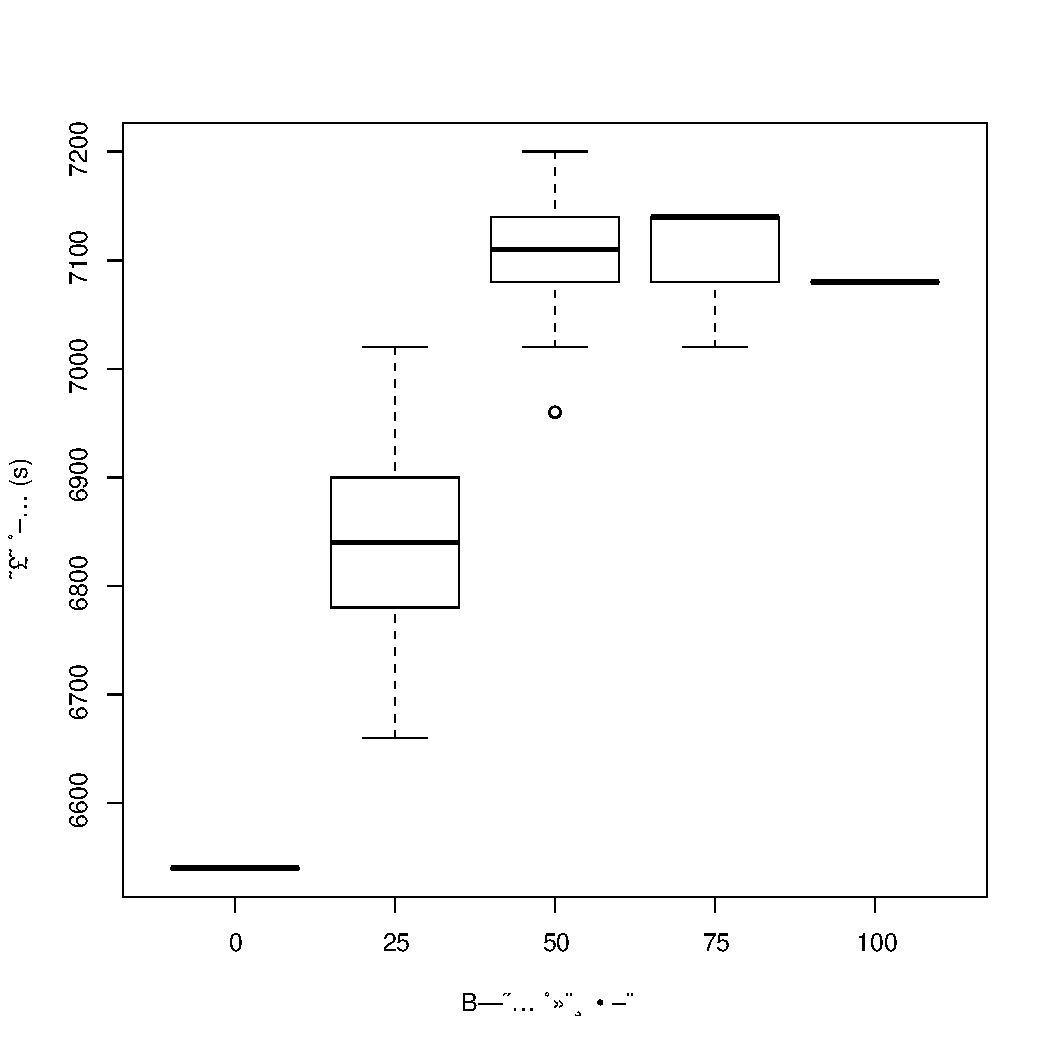
\includegraphics[width=0.5\linewidth]{factor2_box_ttime}
% \caption{最大减速度影响下模拟用时箱图}
% \label{factor2_box_ttime}
% \end{center}
% \end{figure}

% \autoref{factor2_box_ttime}给出了,期望速度影响下模拟总用时的变化,随着\autoref{decel-factor}中最大减速度较大的B型驾驶人的增加,模拟所用时间呈现上升的趋势。对于单纯类型的驾驶人组合,最大减速度由2.33$m/s^2$增加4.29$m/s^2$,增加84\%,模拟用时从6540s增加到7080s,增加了8.3\%。少量的B型驾驶人即可对总模拟用时造成较大影响,并且使得模拟时间具有很大随机性。


% \begin{figure}[!htb]%
% \centering
% \subfloat[][]{
% \label{factor2_vq_per0}%
% 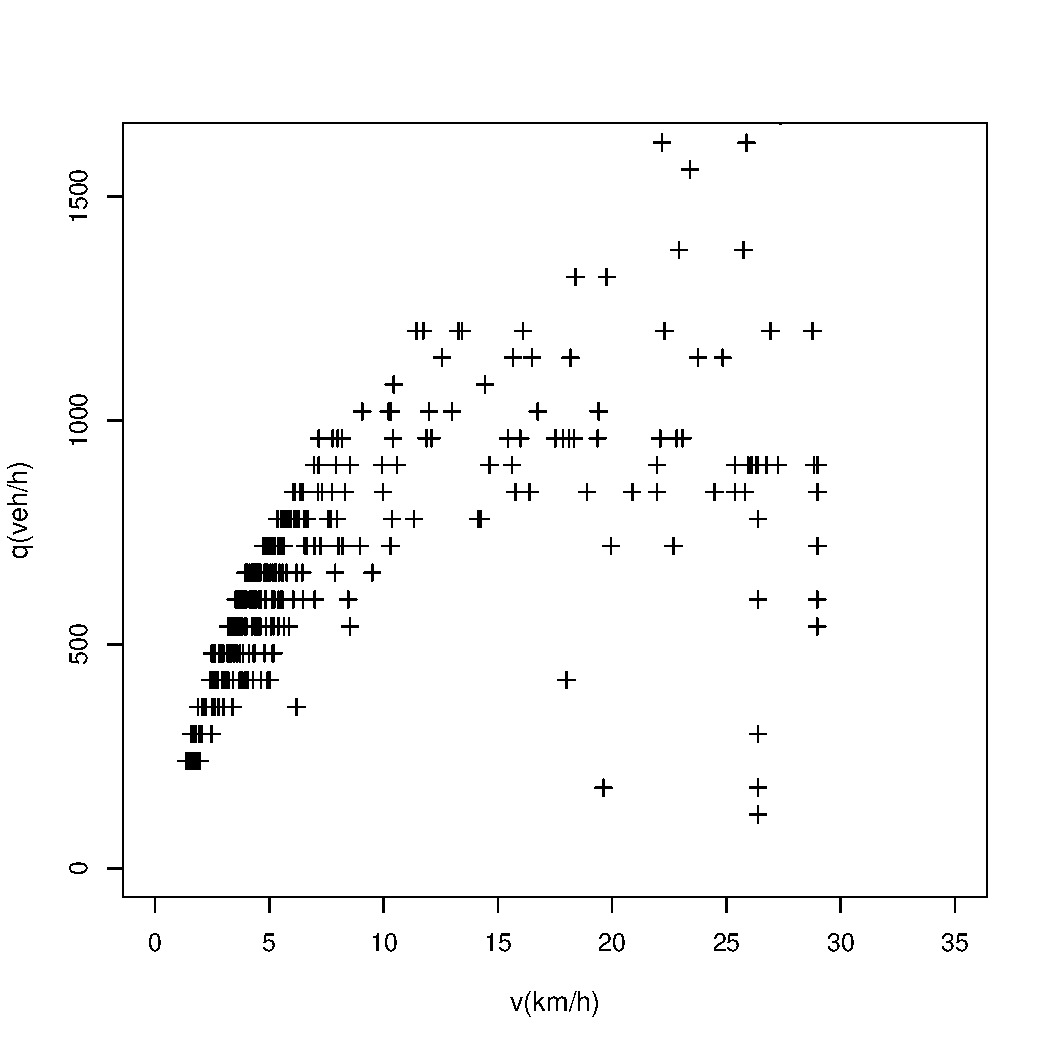
\includegraphics[width=0.25\linewidth]{factor2_vq_per0}
% }%
% \subfloat[][]{%
% \label{factor2_vq_per25}%
% 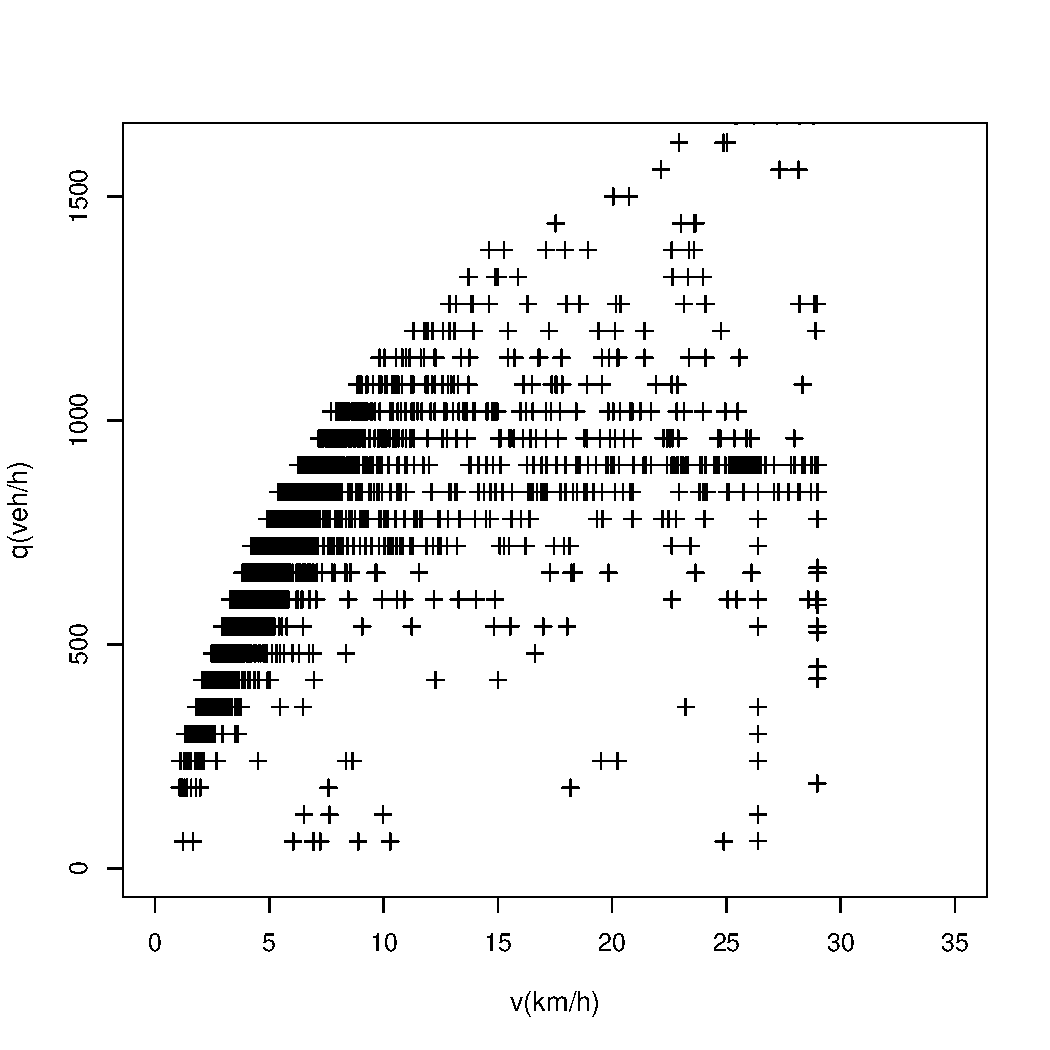
\includegraphics[width=0.25\linewidth]{factor2_vq_per25}}
% \subfloat[][]{%
% \label{factor2_vq_per50}%
% 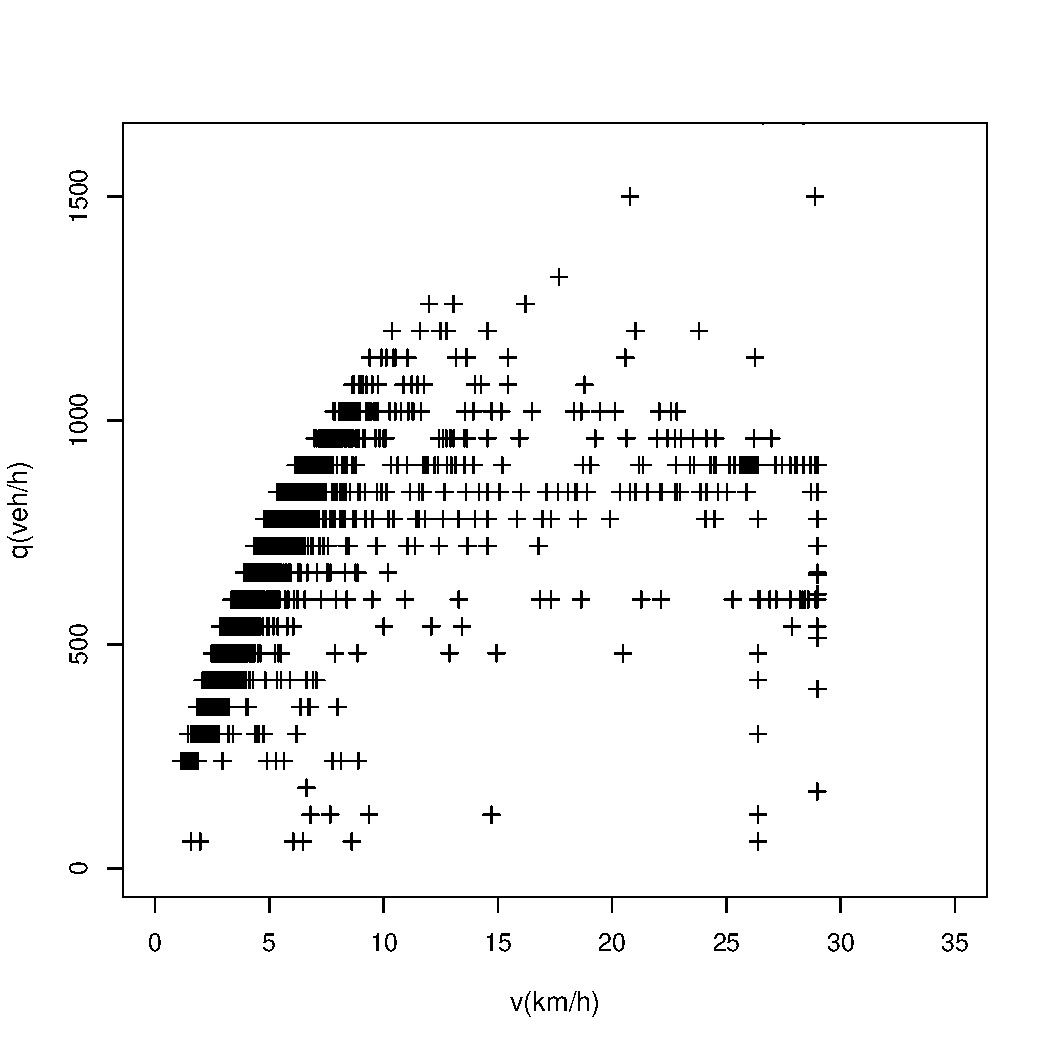
\includegraphics[width=0.25\linewidth]{factor2_vq_per50}}\\%
% \subfloat[][]{%
% \label{factor2_vq_per75}%
% 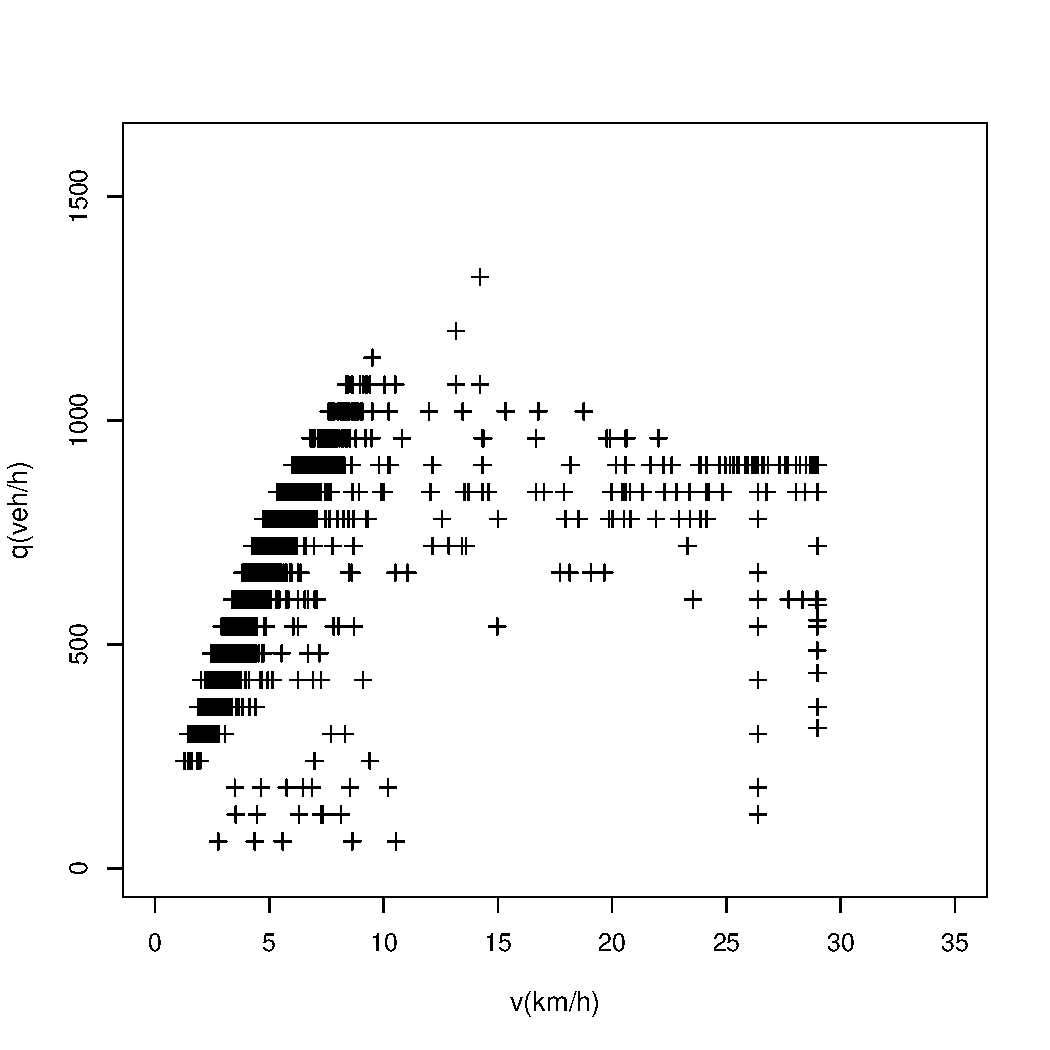
\includegraphics[width=0.25\linewidth]{factor2_vq_per75}}%
% \subfloat[][]{%
% \label{factor2_vq_per100}%
% 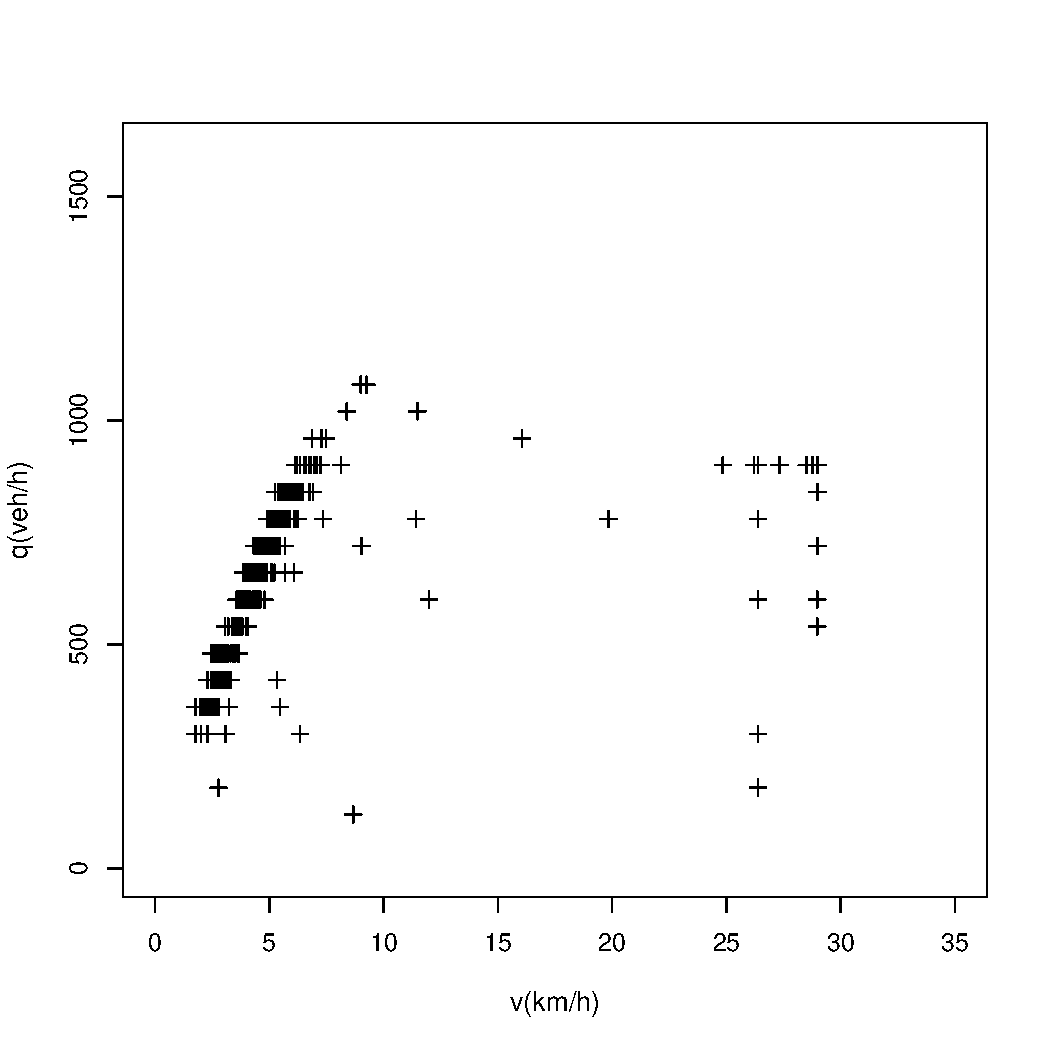
\includegraphics[width=0.25\linewidth]{factor2_vq_per100}}
% \caption[A set of four sub-floats.]{最大减速度影响下速度流量关系图
% \subref{factor2_vq_per0}
% \subref{factor2_vq_per25} 
% \subref{factor2_vq_per50}
% \subref{factor2_vq_per75}
% \subref{factor2_vq_per100}分别表示\autoref{decel-factor}中的B型驾驶人的百分比分别为0\%,25\%,50\%,75\%,100\%}%
% \label{factor2_vq}%
% \end{figure}



% \begin{figure}[!htb]%
% \centering
% \subfloat[][]{
% \label{factor2_kq_per0}%
% 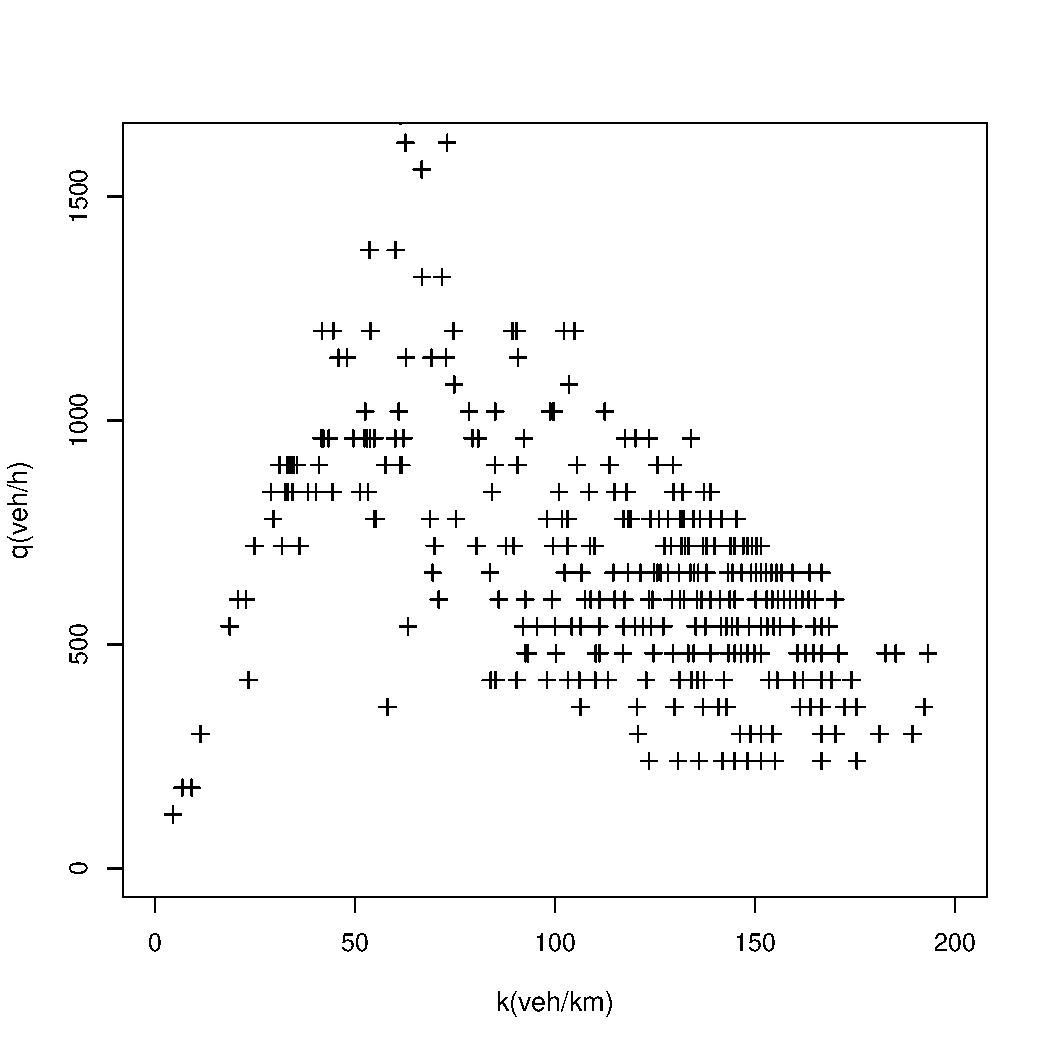
\includegraphics[width=0.25\linewidth]{factor2_kq_per0}
% }%
% \subfloat[][]{%
% \label{factor2_kq_per25}%
% 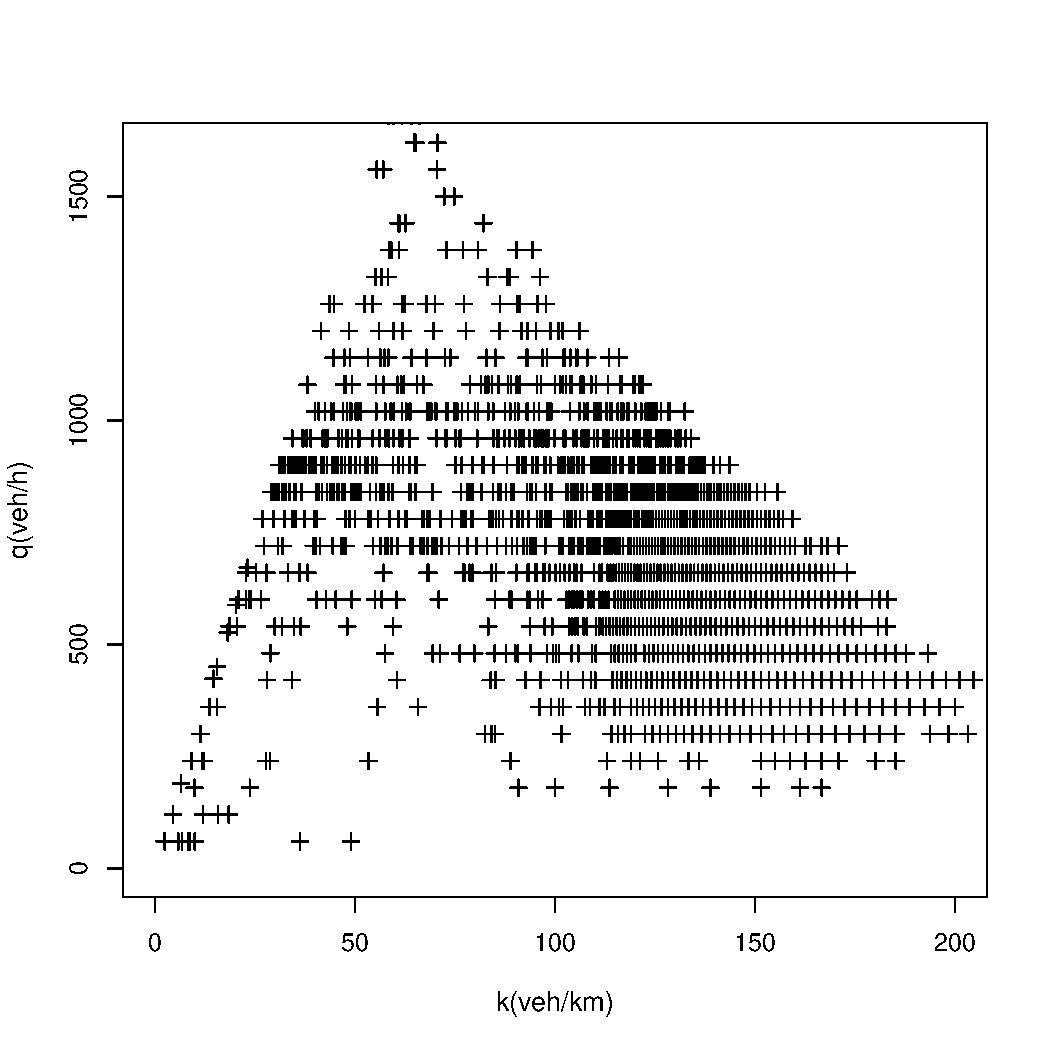
\includegraphics[width=0.25\linewidth]{factor2_kq_per25}}
% \subfloat[][]{%
% \label{factor2_kq_per50}%
% 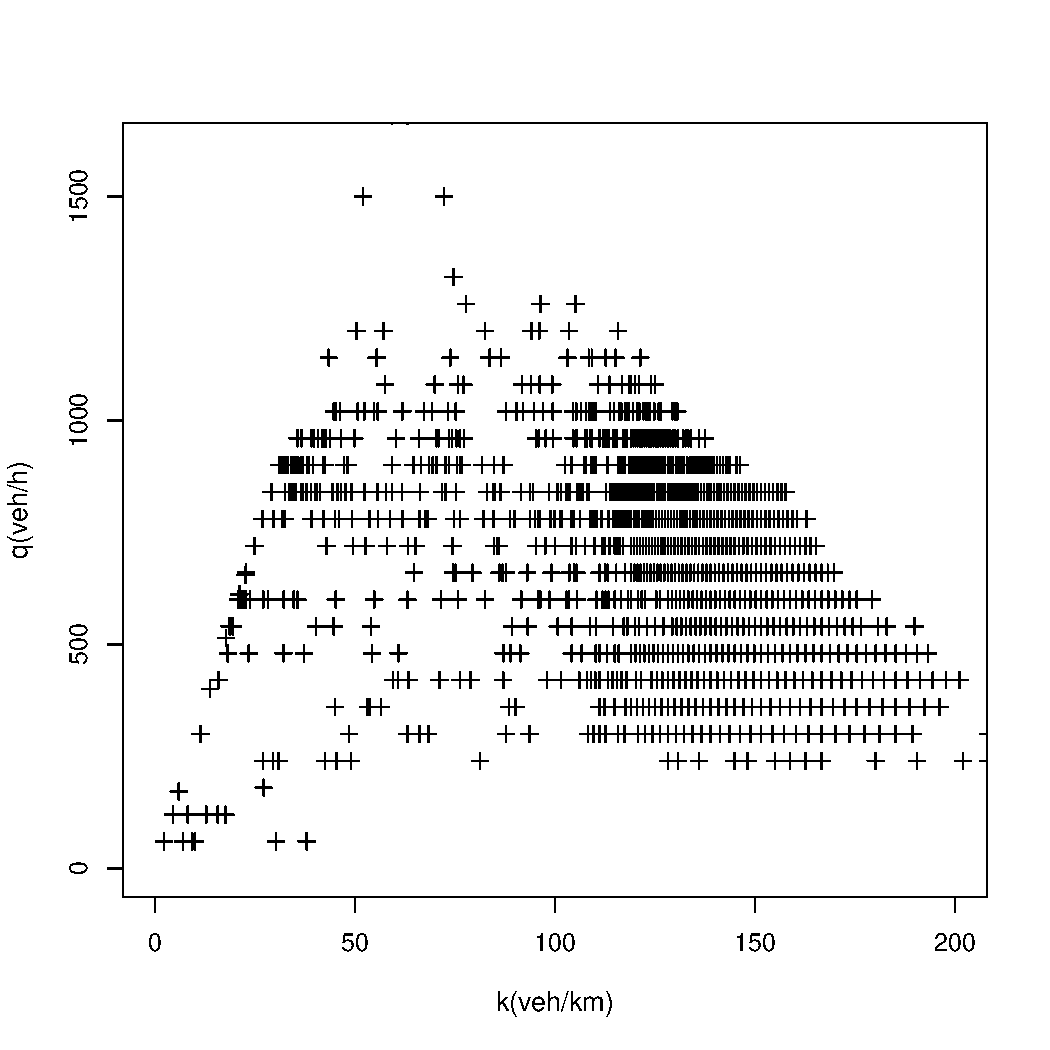
\includegraphics[width=0.25\linewidth]{factor2_kq_per50}}\\%
% \subfloat[][]{%
% \label{factor2_kq_per75}%
% 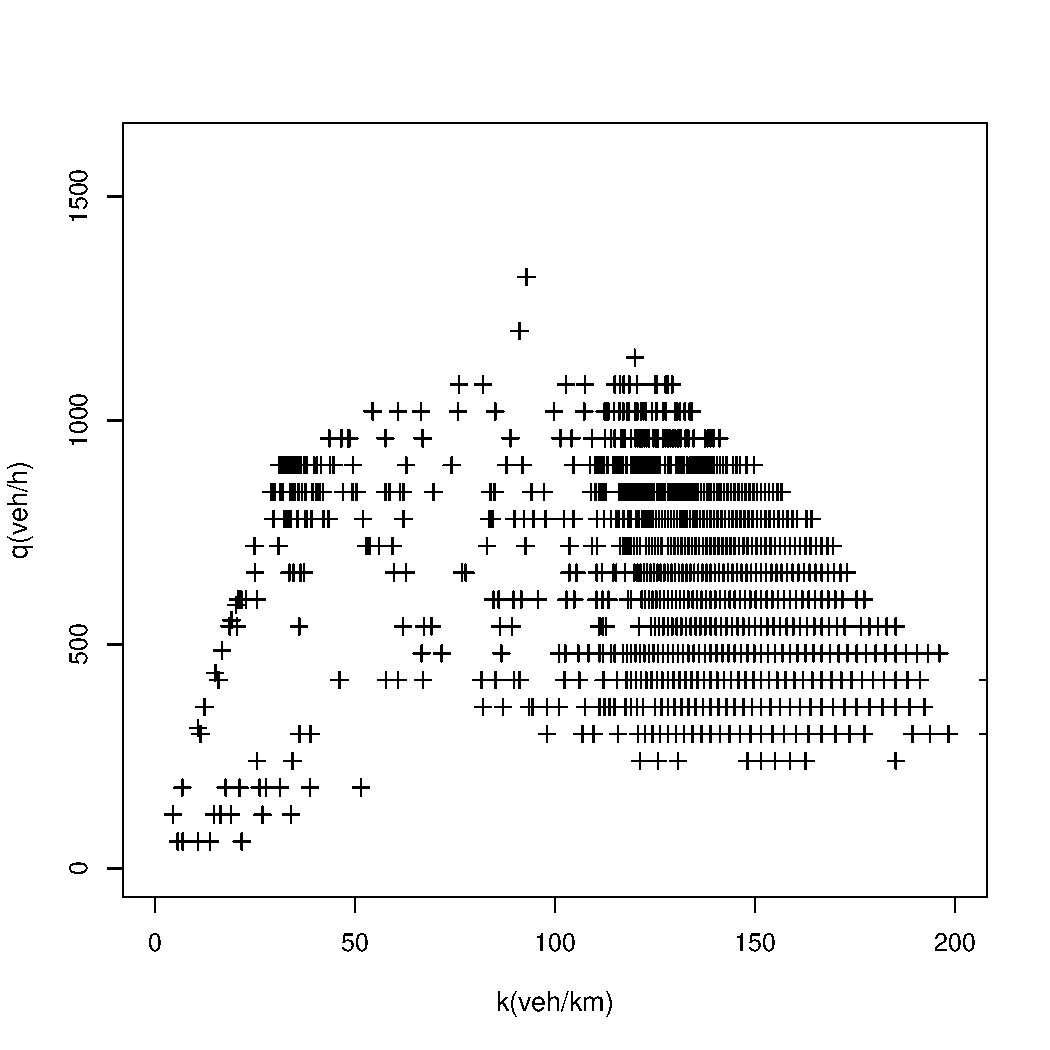
\includegraphics[width=0.25\linewidth]{factor2_kq_per75}}%
% \subfloat[][]{%
% \label{factor2_kq_per100}%
% 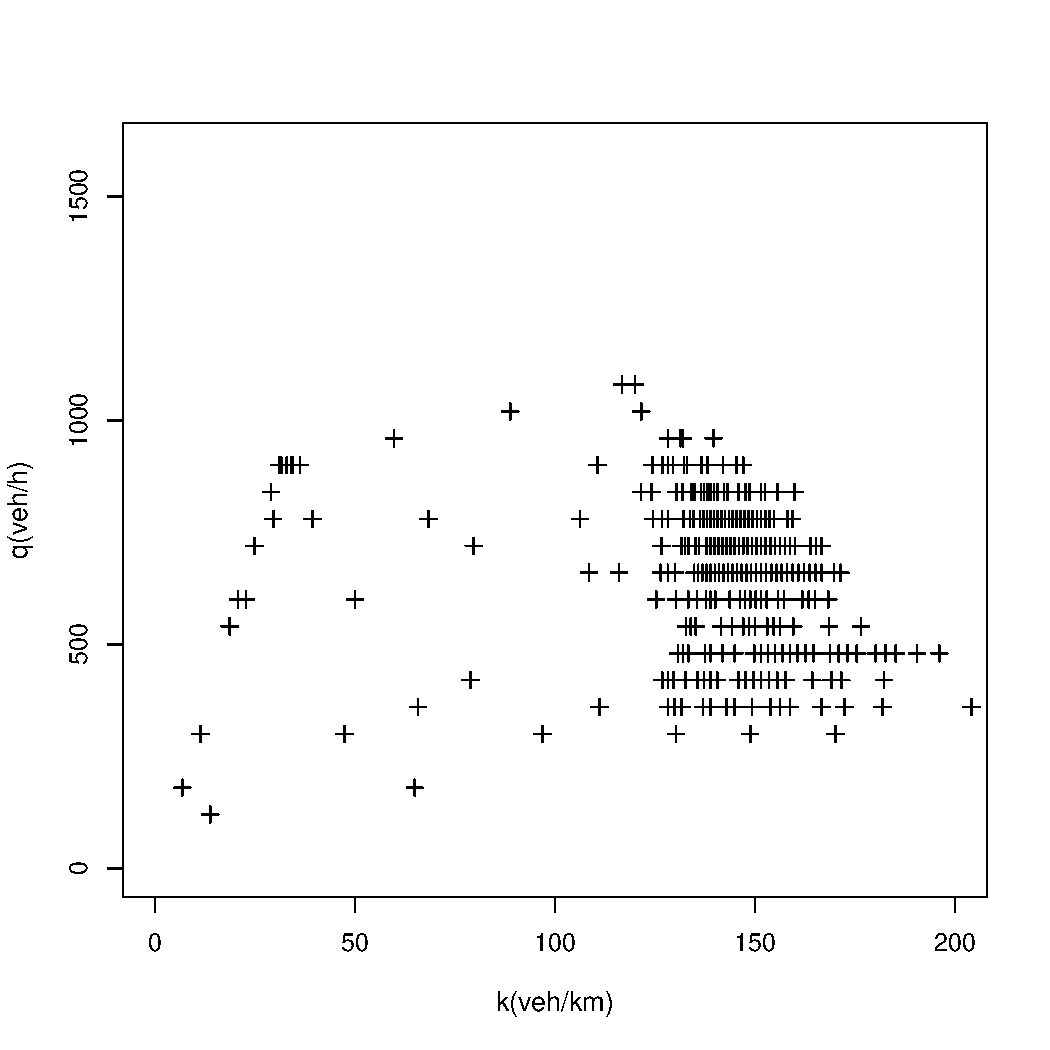
\includegraphics[width=0.25\linewidth]{factor2_kq_per100}}
% \caption[A set of four sub-floats.]{最大减速度影响下的密度流量关系图
% \subref{factor2_kq_per0}
% \subref{factor2_kq_per25} 
% \subref{factor2_kq_per50}
% \subref{factor2_kq_per75}
% \subref{factor2_kq_per100}分别表示\autoref{decel-factor}中的B型驾驶人的百分比分别为0\%,25\%,50\%,75\%,100\%}%
% \label{factor2_kq}%
% \end{figure}

% \autoref{factor2_vq}和\autoref{factor2_kq}给出了,最大减速度影响下速度流量关系图和最大减速度影响下的密度流量关系图,可以看出,随着\autoref{decel-factor}中最大减速度较大的B型驾驶人的比例增加,在速度流量和密度流量关系图上均更难达到最大通行能力。这种趋势随着B型驾驶人的增加而更为明显。



% \begin{figure}[!htb]
% \begin{center}
% 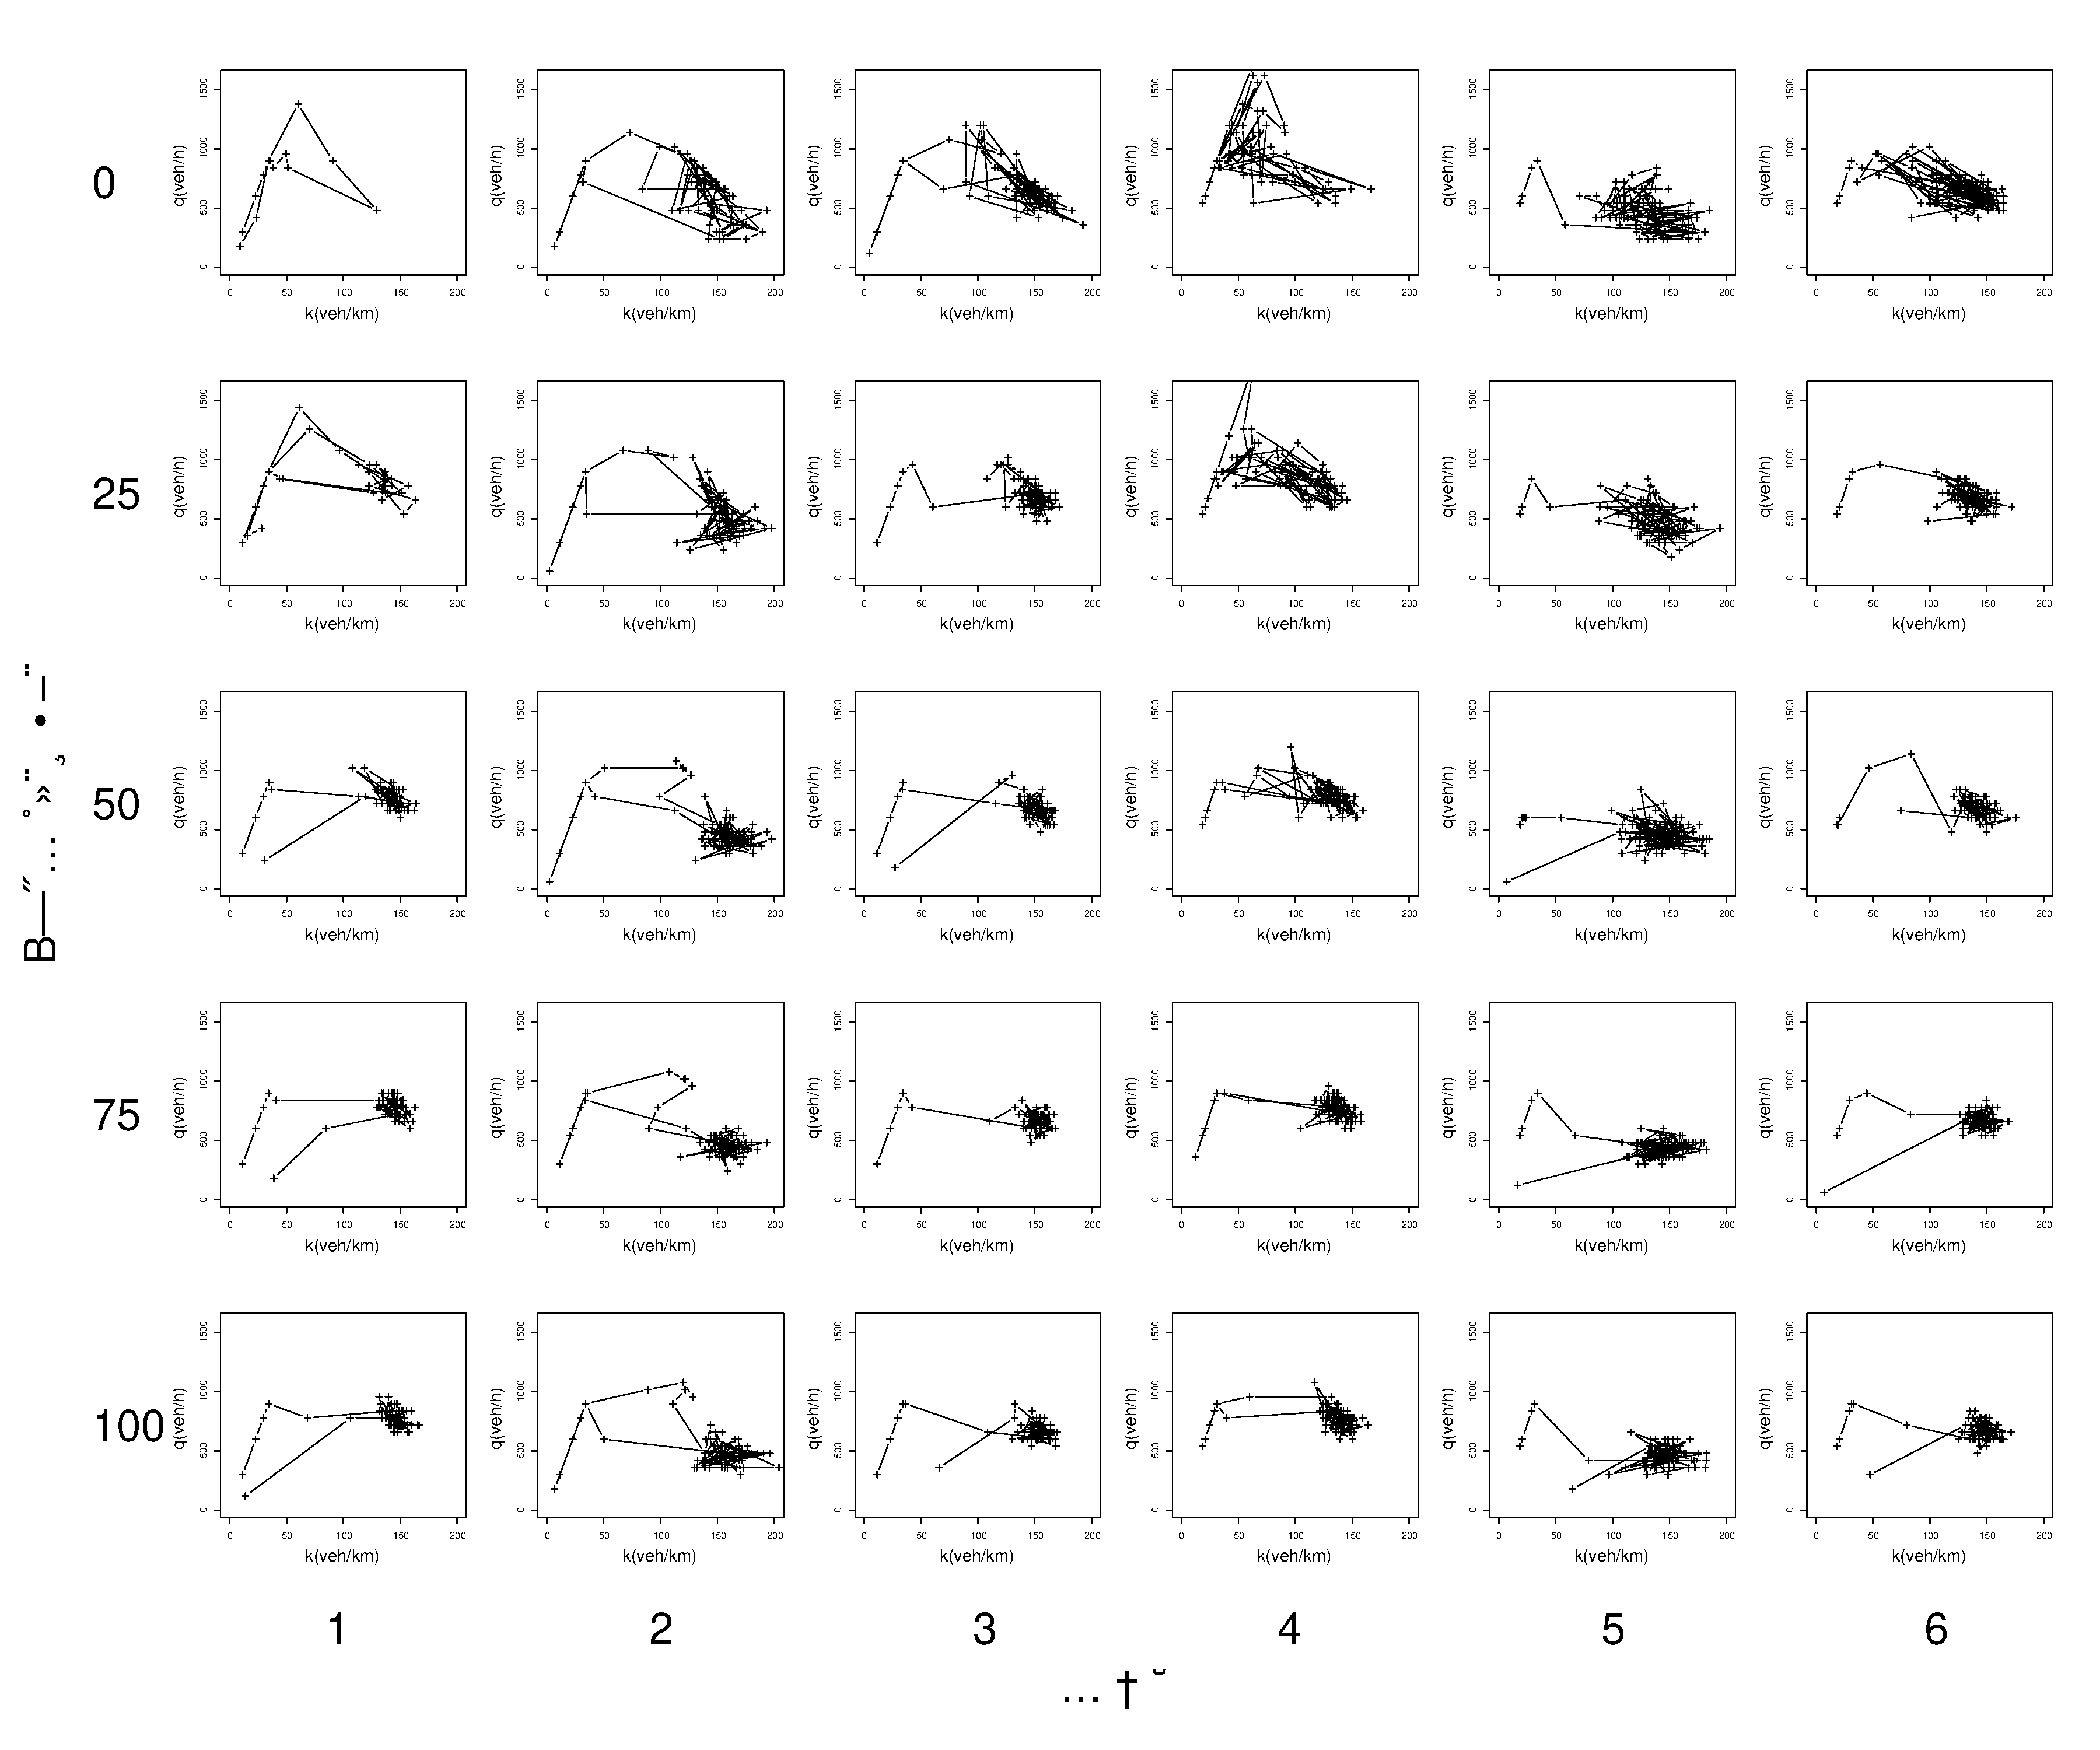
\includegraphics[width=\linewidth]{factor2_kqedges}
% \caption{最大减速度影响下各检测器密度流量关系图}
% \label{factor2_kqedges}
% \end{center}
% \end{figure}

% 最大减速度的增加造成密度流量图上,集中在J线以上,相对不稳定的状态。\autoref{factor2_kqedges}给出了最大减速度影响下各检测器密度流量关系图,从各检测器的密度流量状态跃迁图看,最为明显的是,检测器1和4的最大或接近最大通行能力,随着B型驾驶人的更多的混入,从自由流的状态更多的往同步流状态跃迁。


% \subsection{混合影响因素}

% \autoref{combined_box_ttime},\autoref{combined_vq},\autoref{combined_kq},\autoref{combined_kqedges},分别给出了混合作用影响下模拟用时箱图,速度流量关系图,密度流量关系图和各检测器密度流量关系图。其结果与最大减速度影响下的结果相似,可以推断对交通流效率性的影响,主要的贡献成分来自于最大减速度的影响,最大减速度越大则交通流越难达到最大通行能力,也越多的处于较为不稳定的同步流状态。

% \begin{figure}[!htb]
% \begin{center}
% 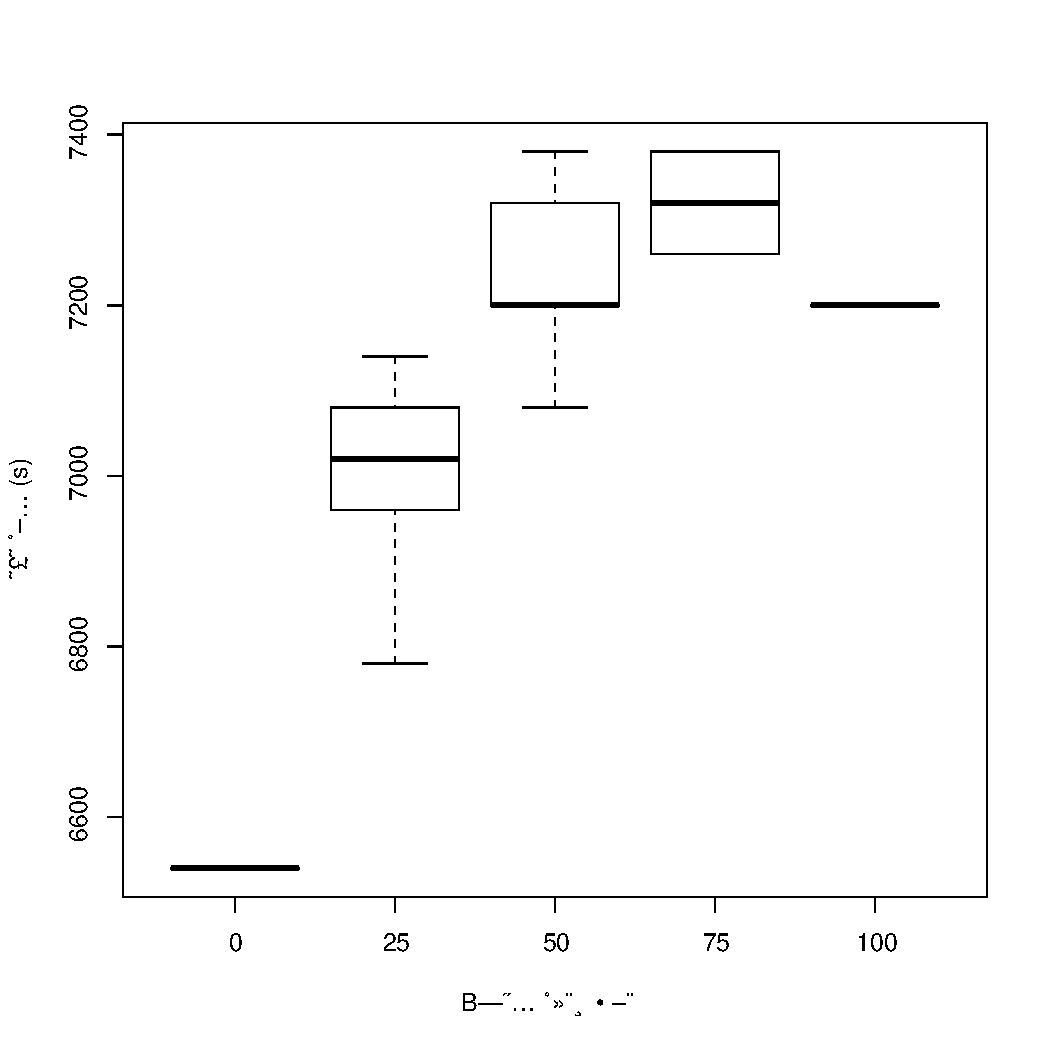
\includegraphics[width=0.5\linewidth]{combined_box_ttime}
% \caption{混合作用影响下模拟用时箱图}
% \label{combined_box_ttime}
% \end{center}
% \end{figure}



% \begin{figure}[!htb]%
% \centering
% \subfloat[][]{
% \label{combined_vq_per0}%
% 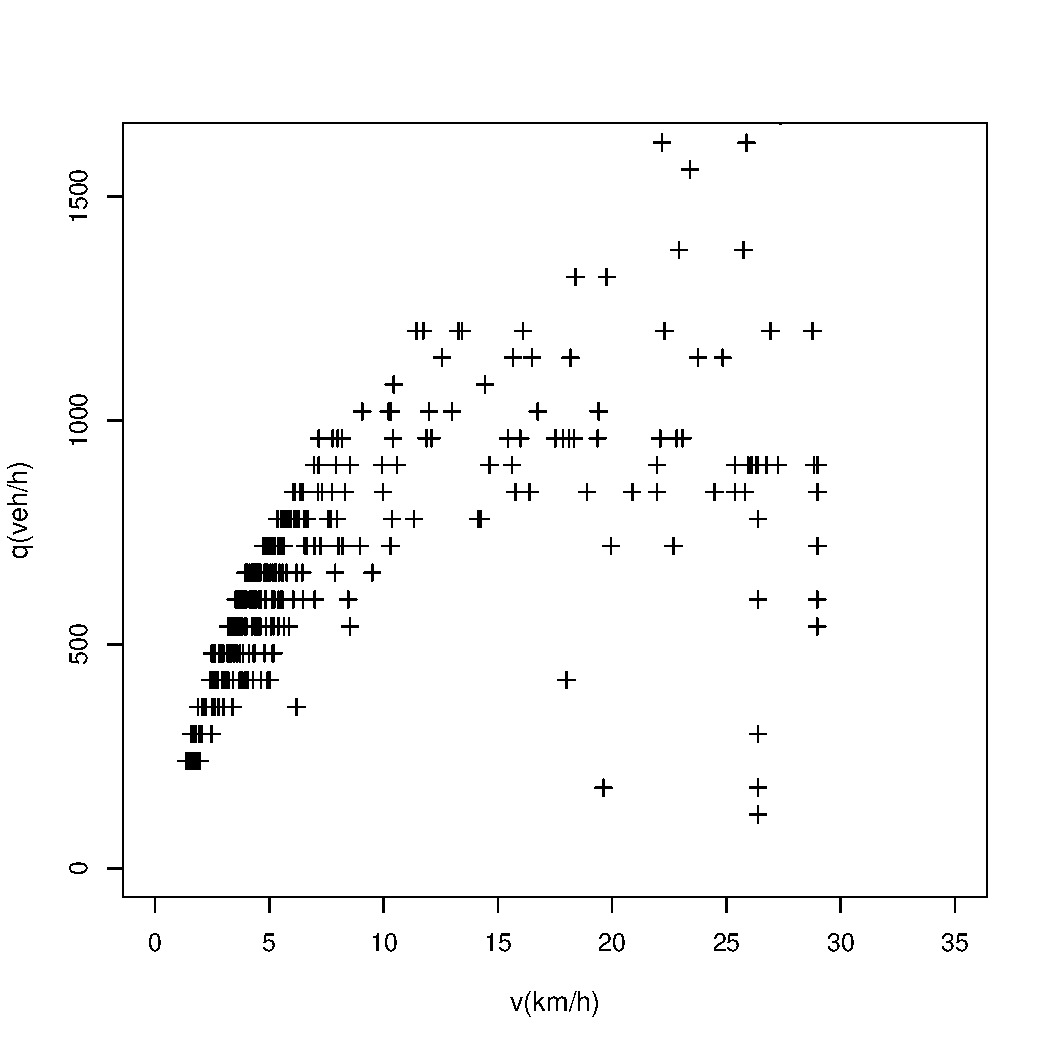
\includegraphics[width=0.25\linewidth]{combined_vq_per0}
% }%
% \subfloat[][]{%
% \label{combined_vq_per25}%
% 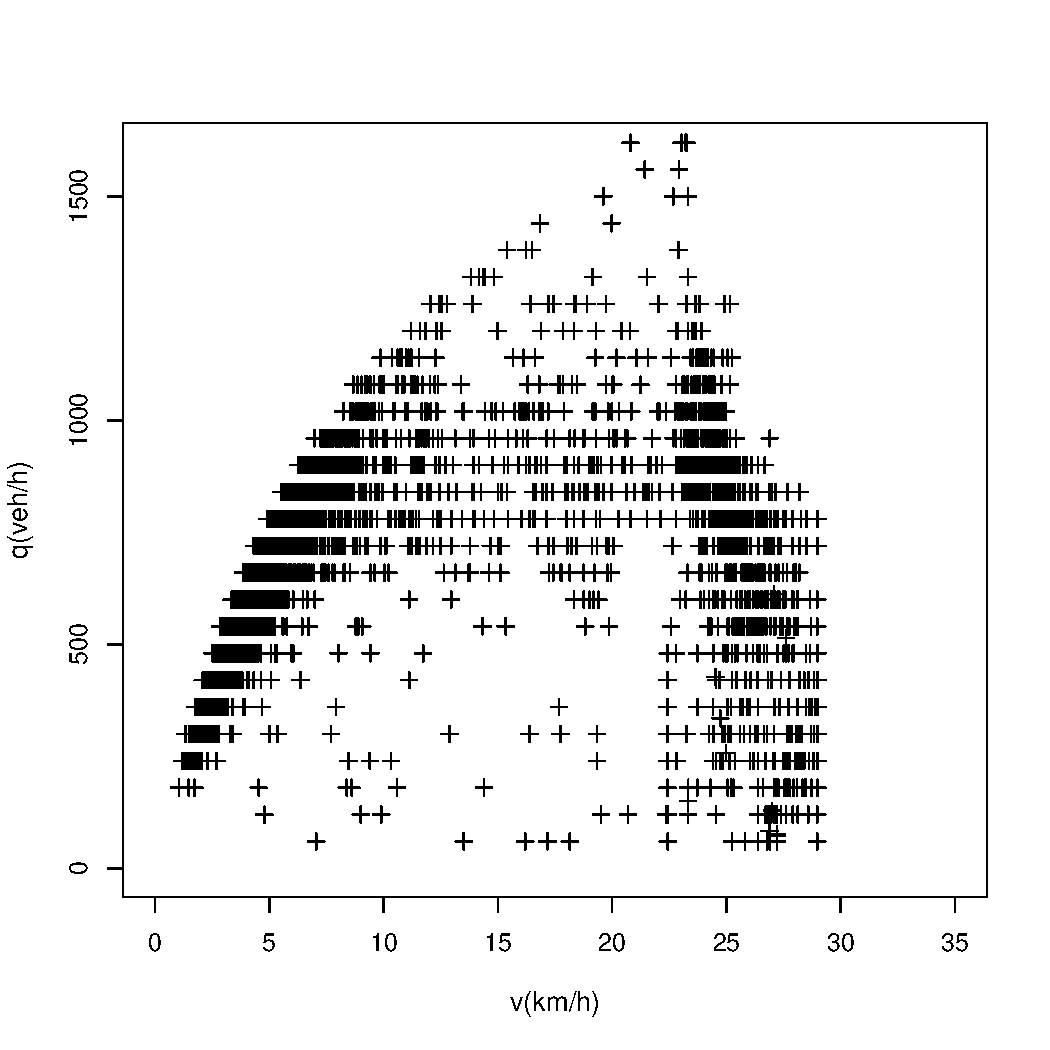
\includegraphics[width=0.25\linewidth]{combined_vq_per25}}
% \subfloat[][]{%
% \label{combined_vq_per50}%
% 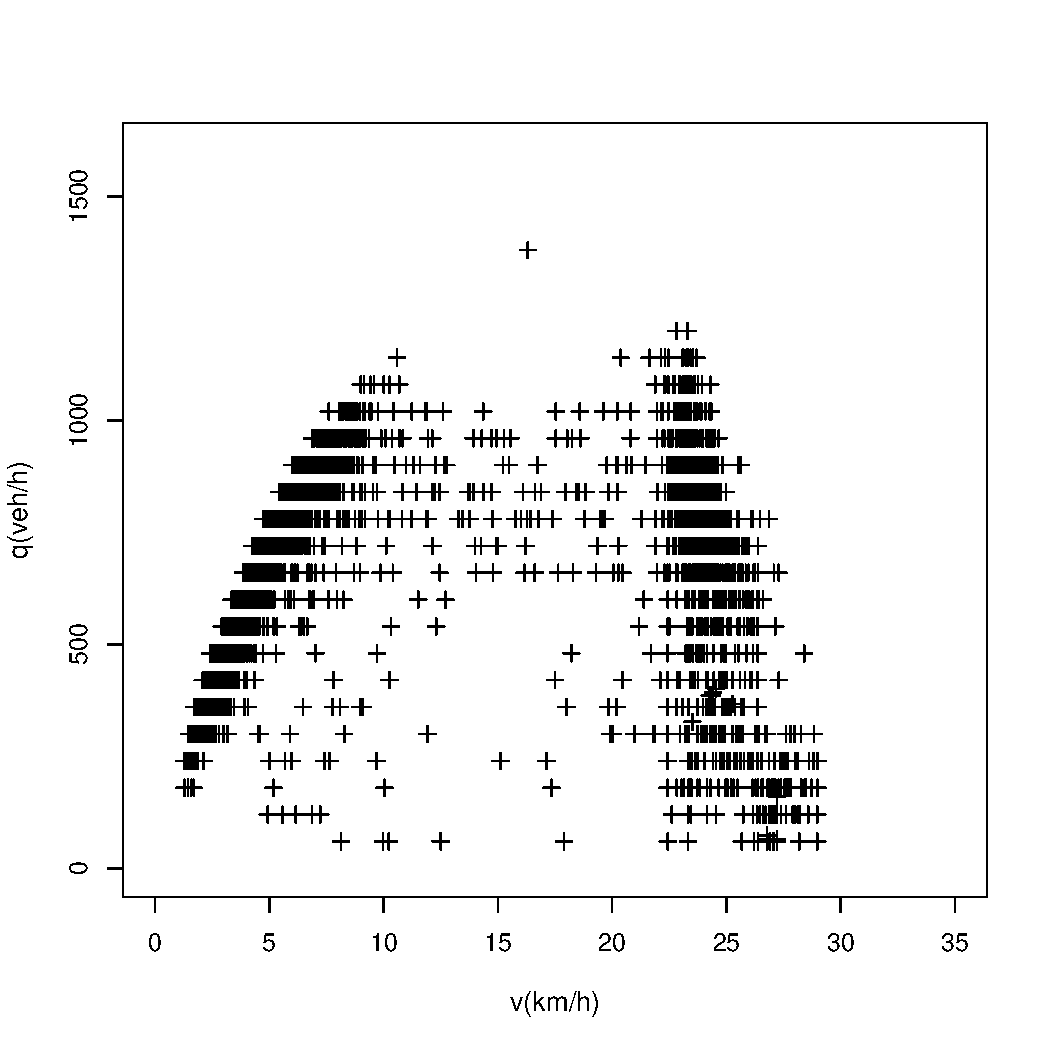
\includegraphics[width=0.25\linewidth]{combined_vq_per50}}\\%
% \subfloat[][]{%
% \label{combined_vq_per75}%
% 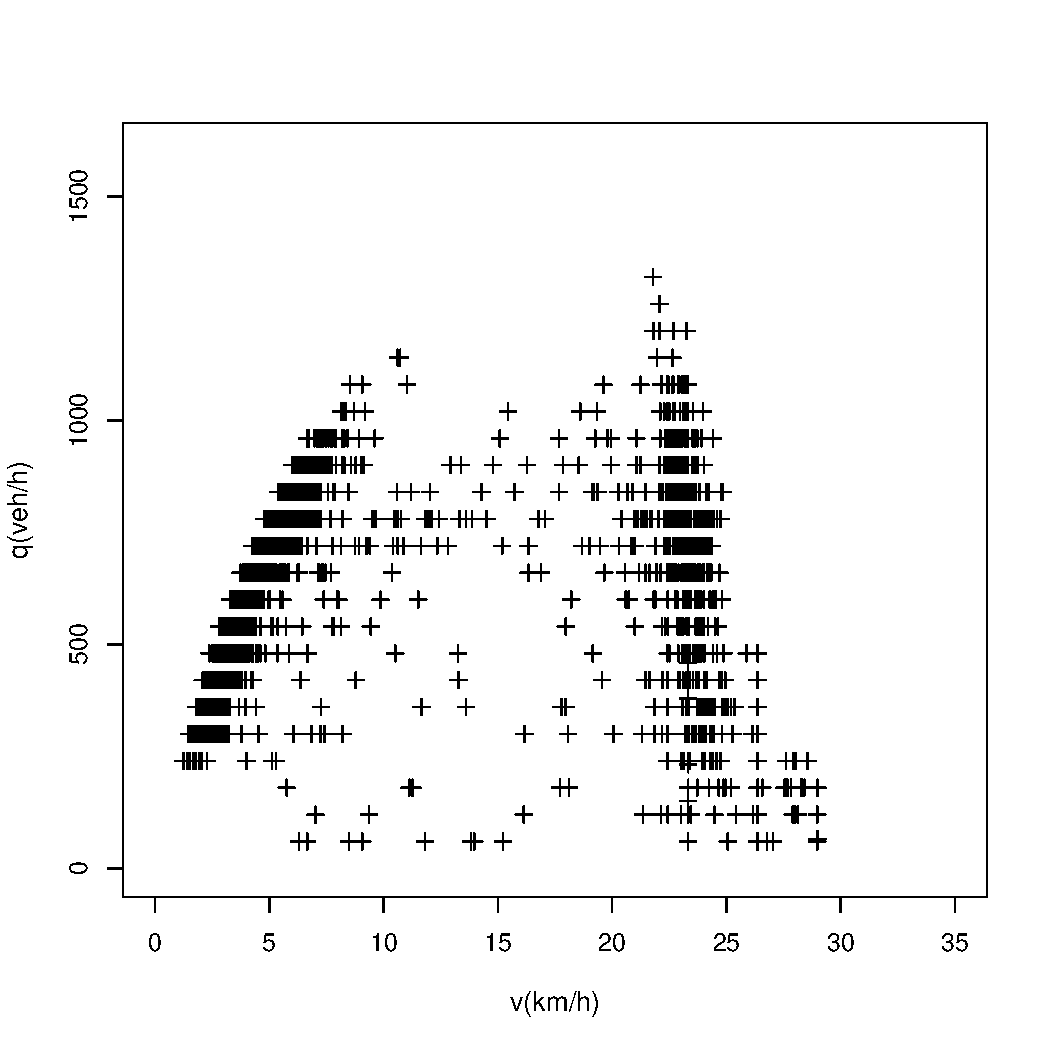
\includegraphics[width=0.25\linewidth]{combined_vq_per75}}%
% \subfloat[][]{%
% \label{combined_vq_per100}%
% 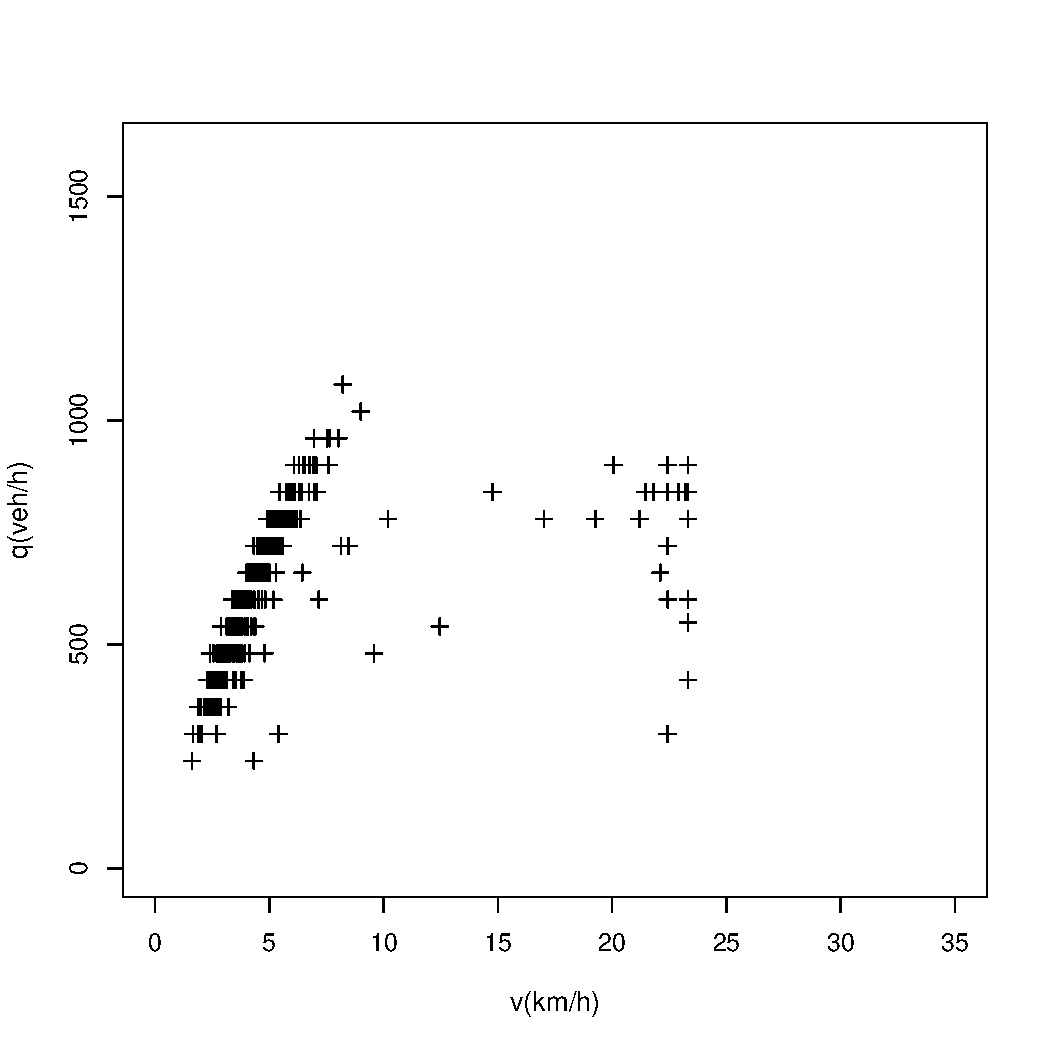
\includegraphics[width=0.25\linewidth]{combined_vq_per100}}
% \caption[A set of four sub-floats.]{混合作用影响下速度流量关系图
% \subref{combined_vq_per0}
% \subref{combined_vq_per25} 
% \subref{combined_vq_per50}
% \subref{combined_vq_per75}
% \subref{combined_vq_per100}分别表示\autoref{combined-factor}中的B型驾驶人的百分比分别为0\%,25\%,50\%,75\%,100\%}%
% \label{combined_vq}%
% \end{figure}


% \begin{figure}[!htb]%
% \centering
% \subfloat[][]{
% \label{combined_kq_per0}%
% 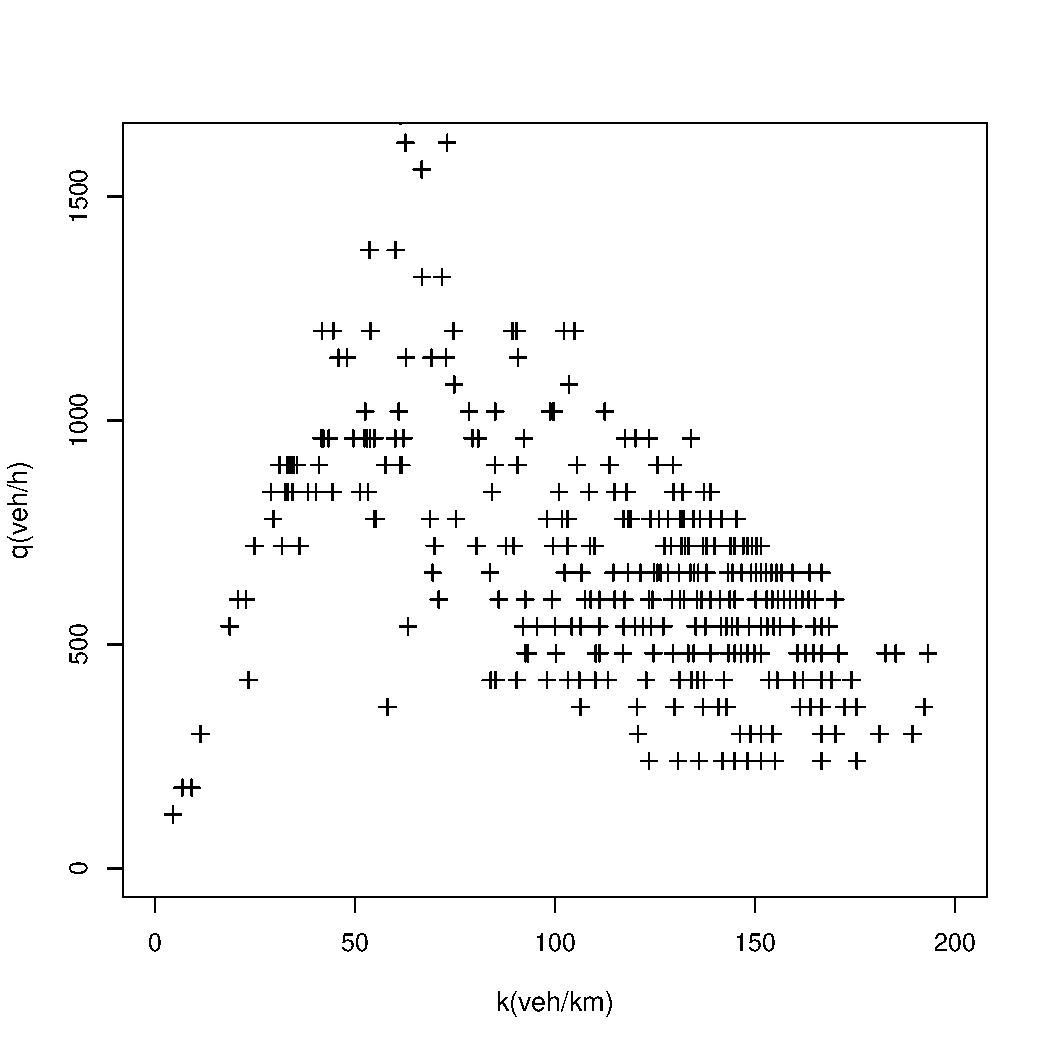
\includegraphics[width=0.25\linewidth]{combined_kq_per0}
% }%
% \subfloat[][]{%
% \label{combined_kq_per25}%
% 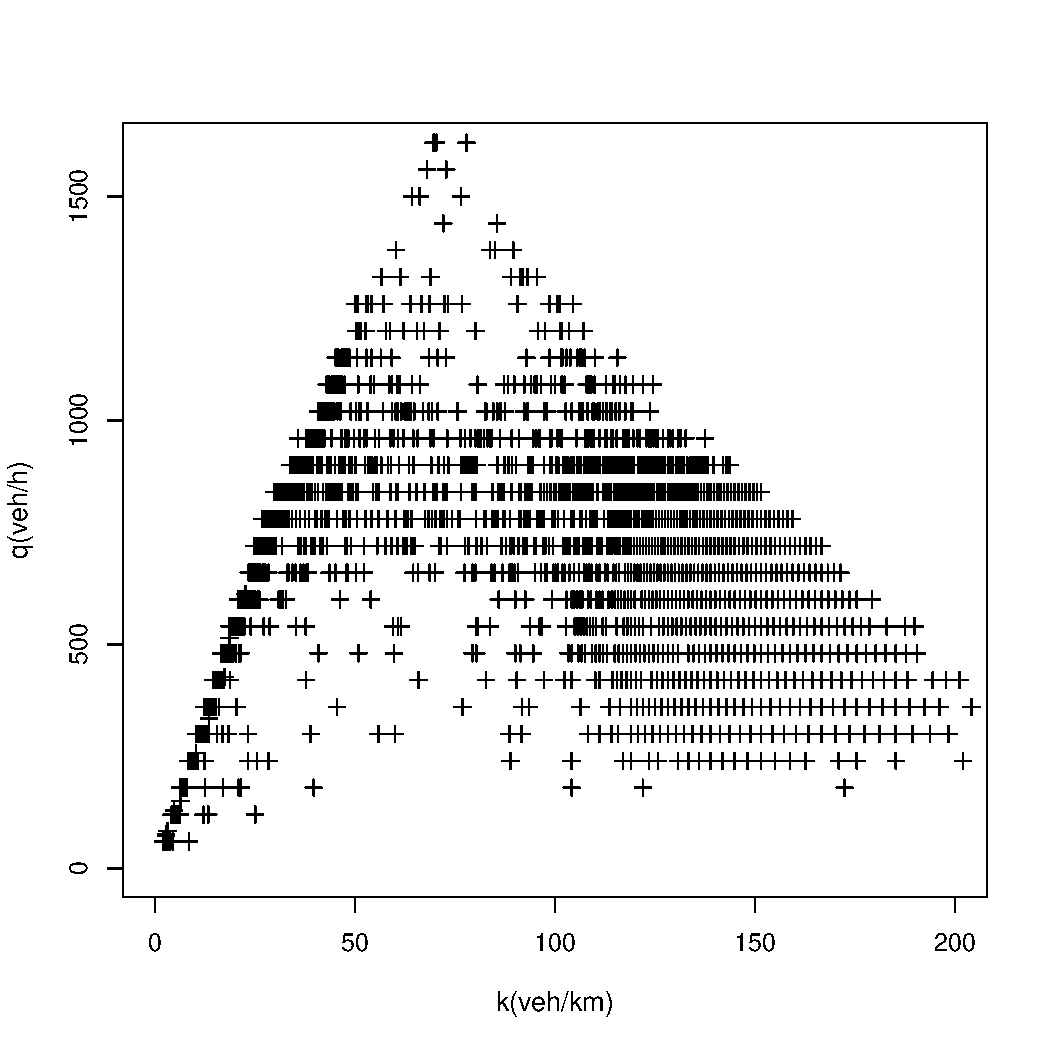
\includegraphics[width=0.25\linewidth]{combined_kq_per25}}
% \subfloat[][]{%
% \label{combined_kq_per50}%
% 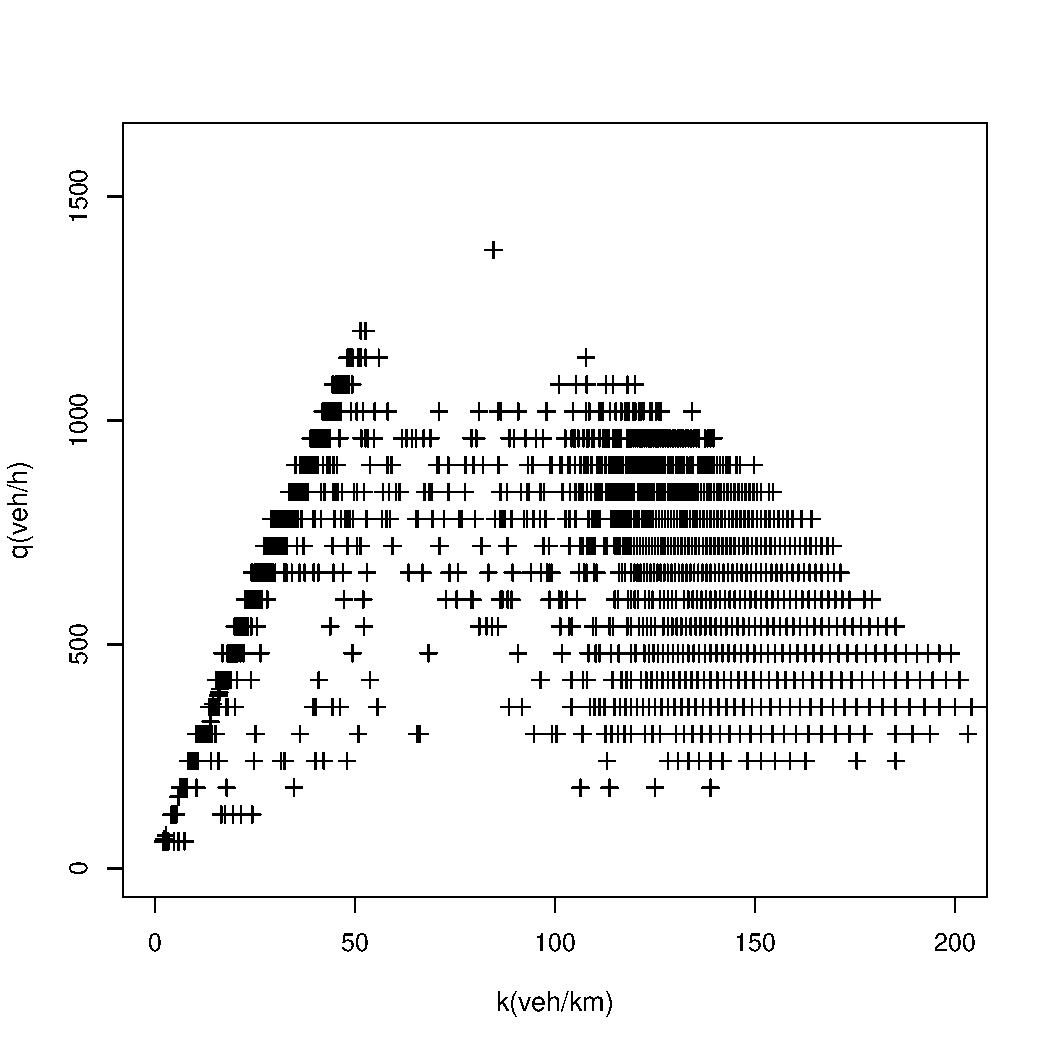
\includegraphics[width=0.25\linewidth]{combined_kq_per50}}\\%
% \subfloat[][]{%
% \label{combined_kq_per75}%
% 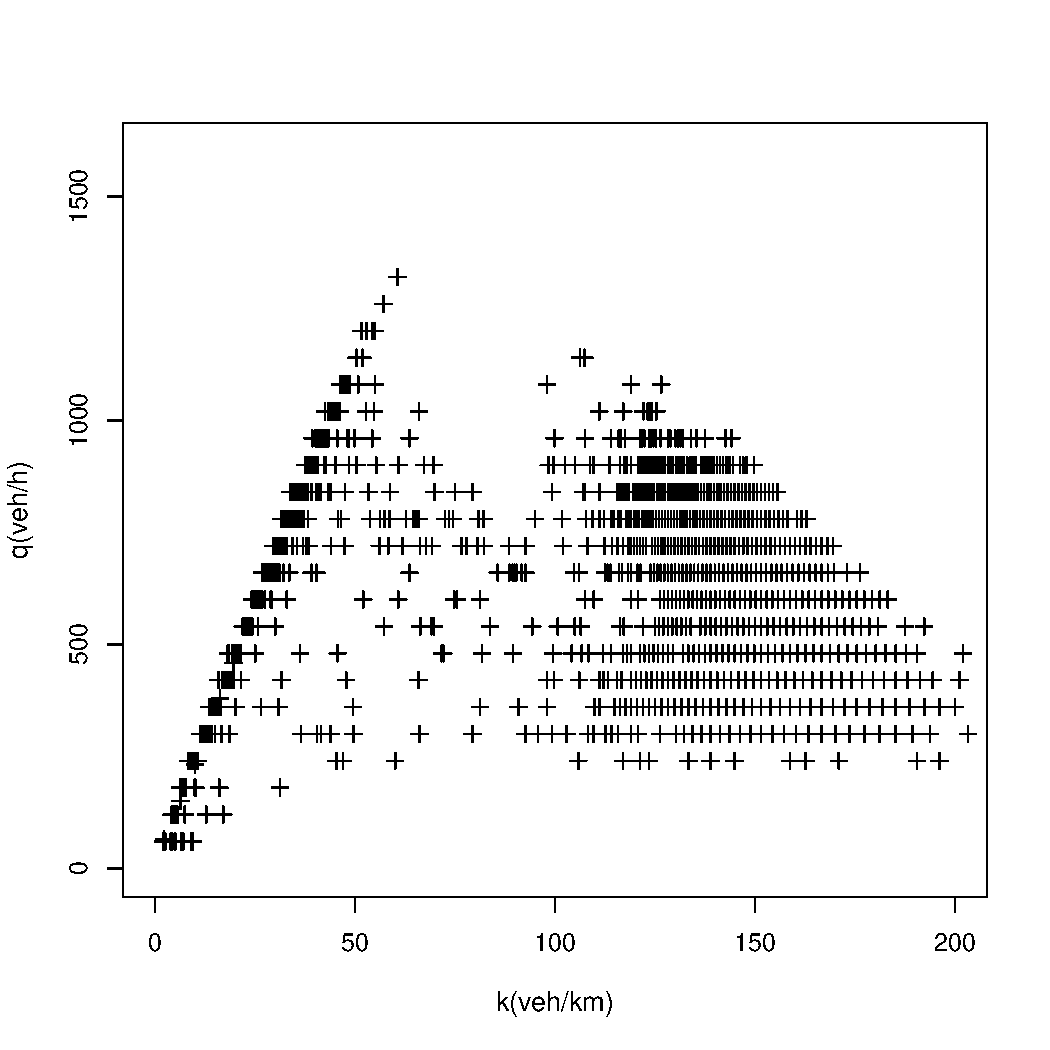
\includegraphics[width=0.25\linewidth]{combined_kq_per75}}%
% \subfloat[][]{%
% \label{combined_kq_per100}%
% 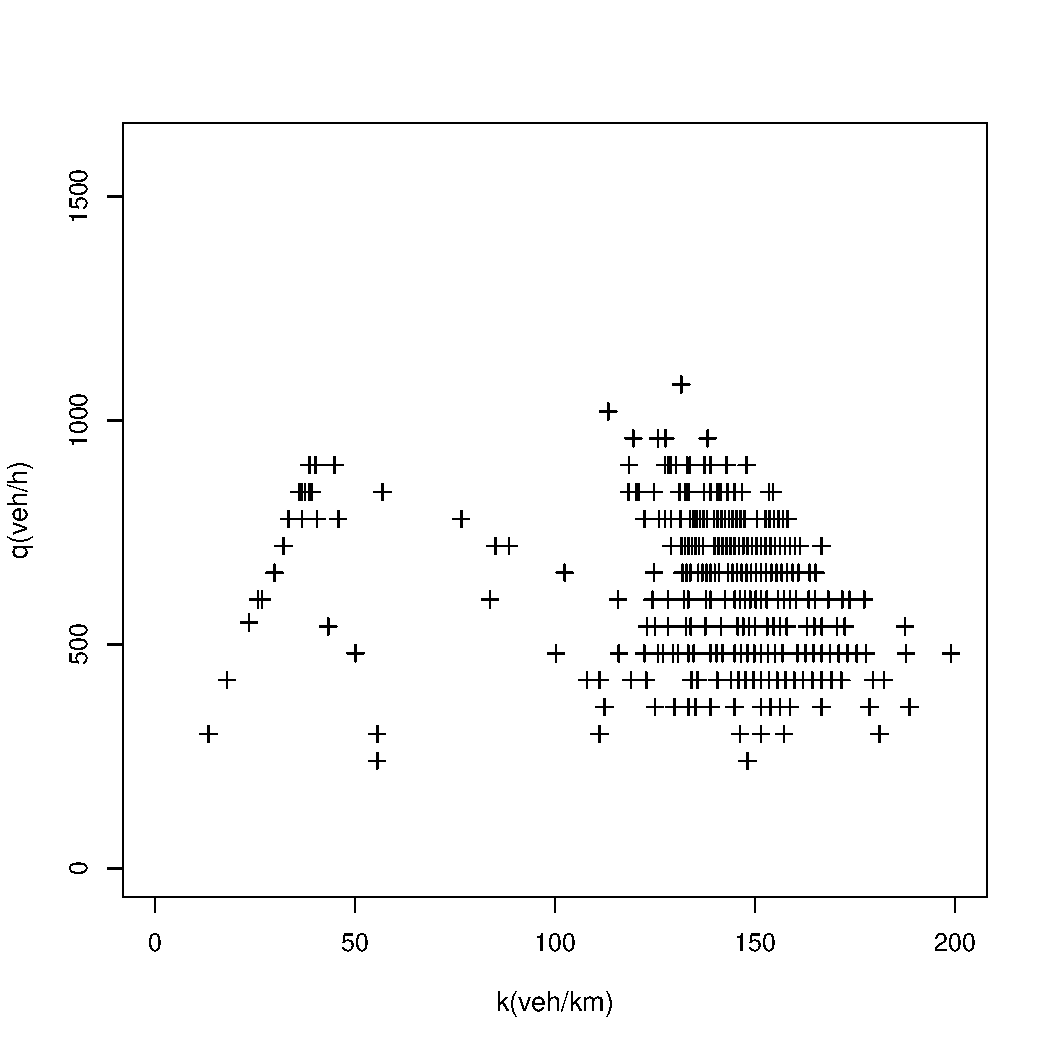
\includegraphics[width=0.25\linewidth]{combined_kq_per100}}
% \caption[A set of four sub-floats.]{混合作用影响下的密度流量关系图
% \subref{combined_kq_per0}
% \subref{combined_kq_per25} 
% \subref{combined_kq_per50}
% \subref{combined_kq_per75}
% \subref{combined_kq_per100}分别表示\autoref{combined-factor}中的B型驾驶人的百分比分别为0\%,25\%,50\%,75\%,100\%}%
% \label{combined_kq}%
% \end{figure}

% \begin{figure}[!htb]
% \begin{center}
% 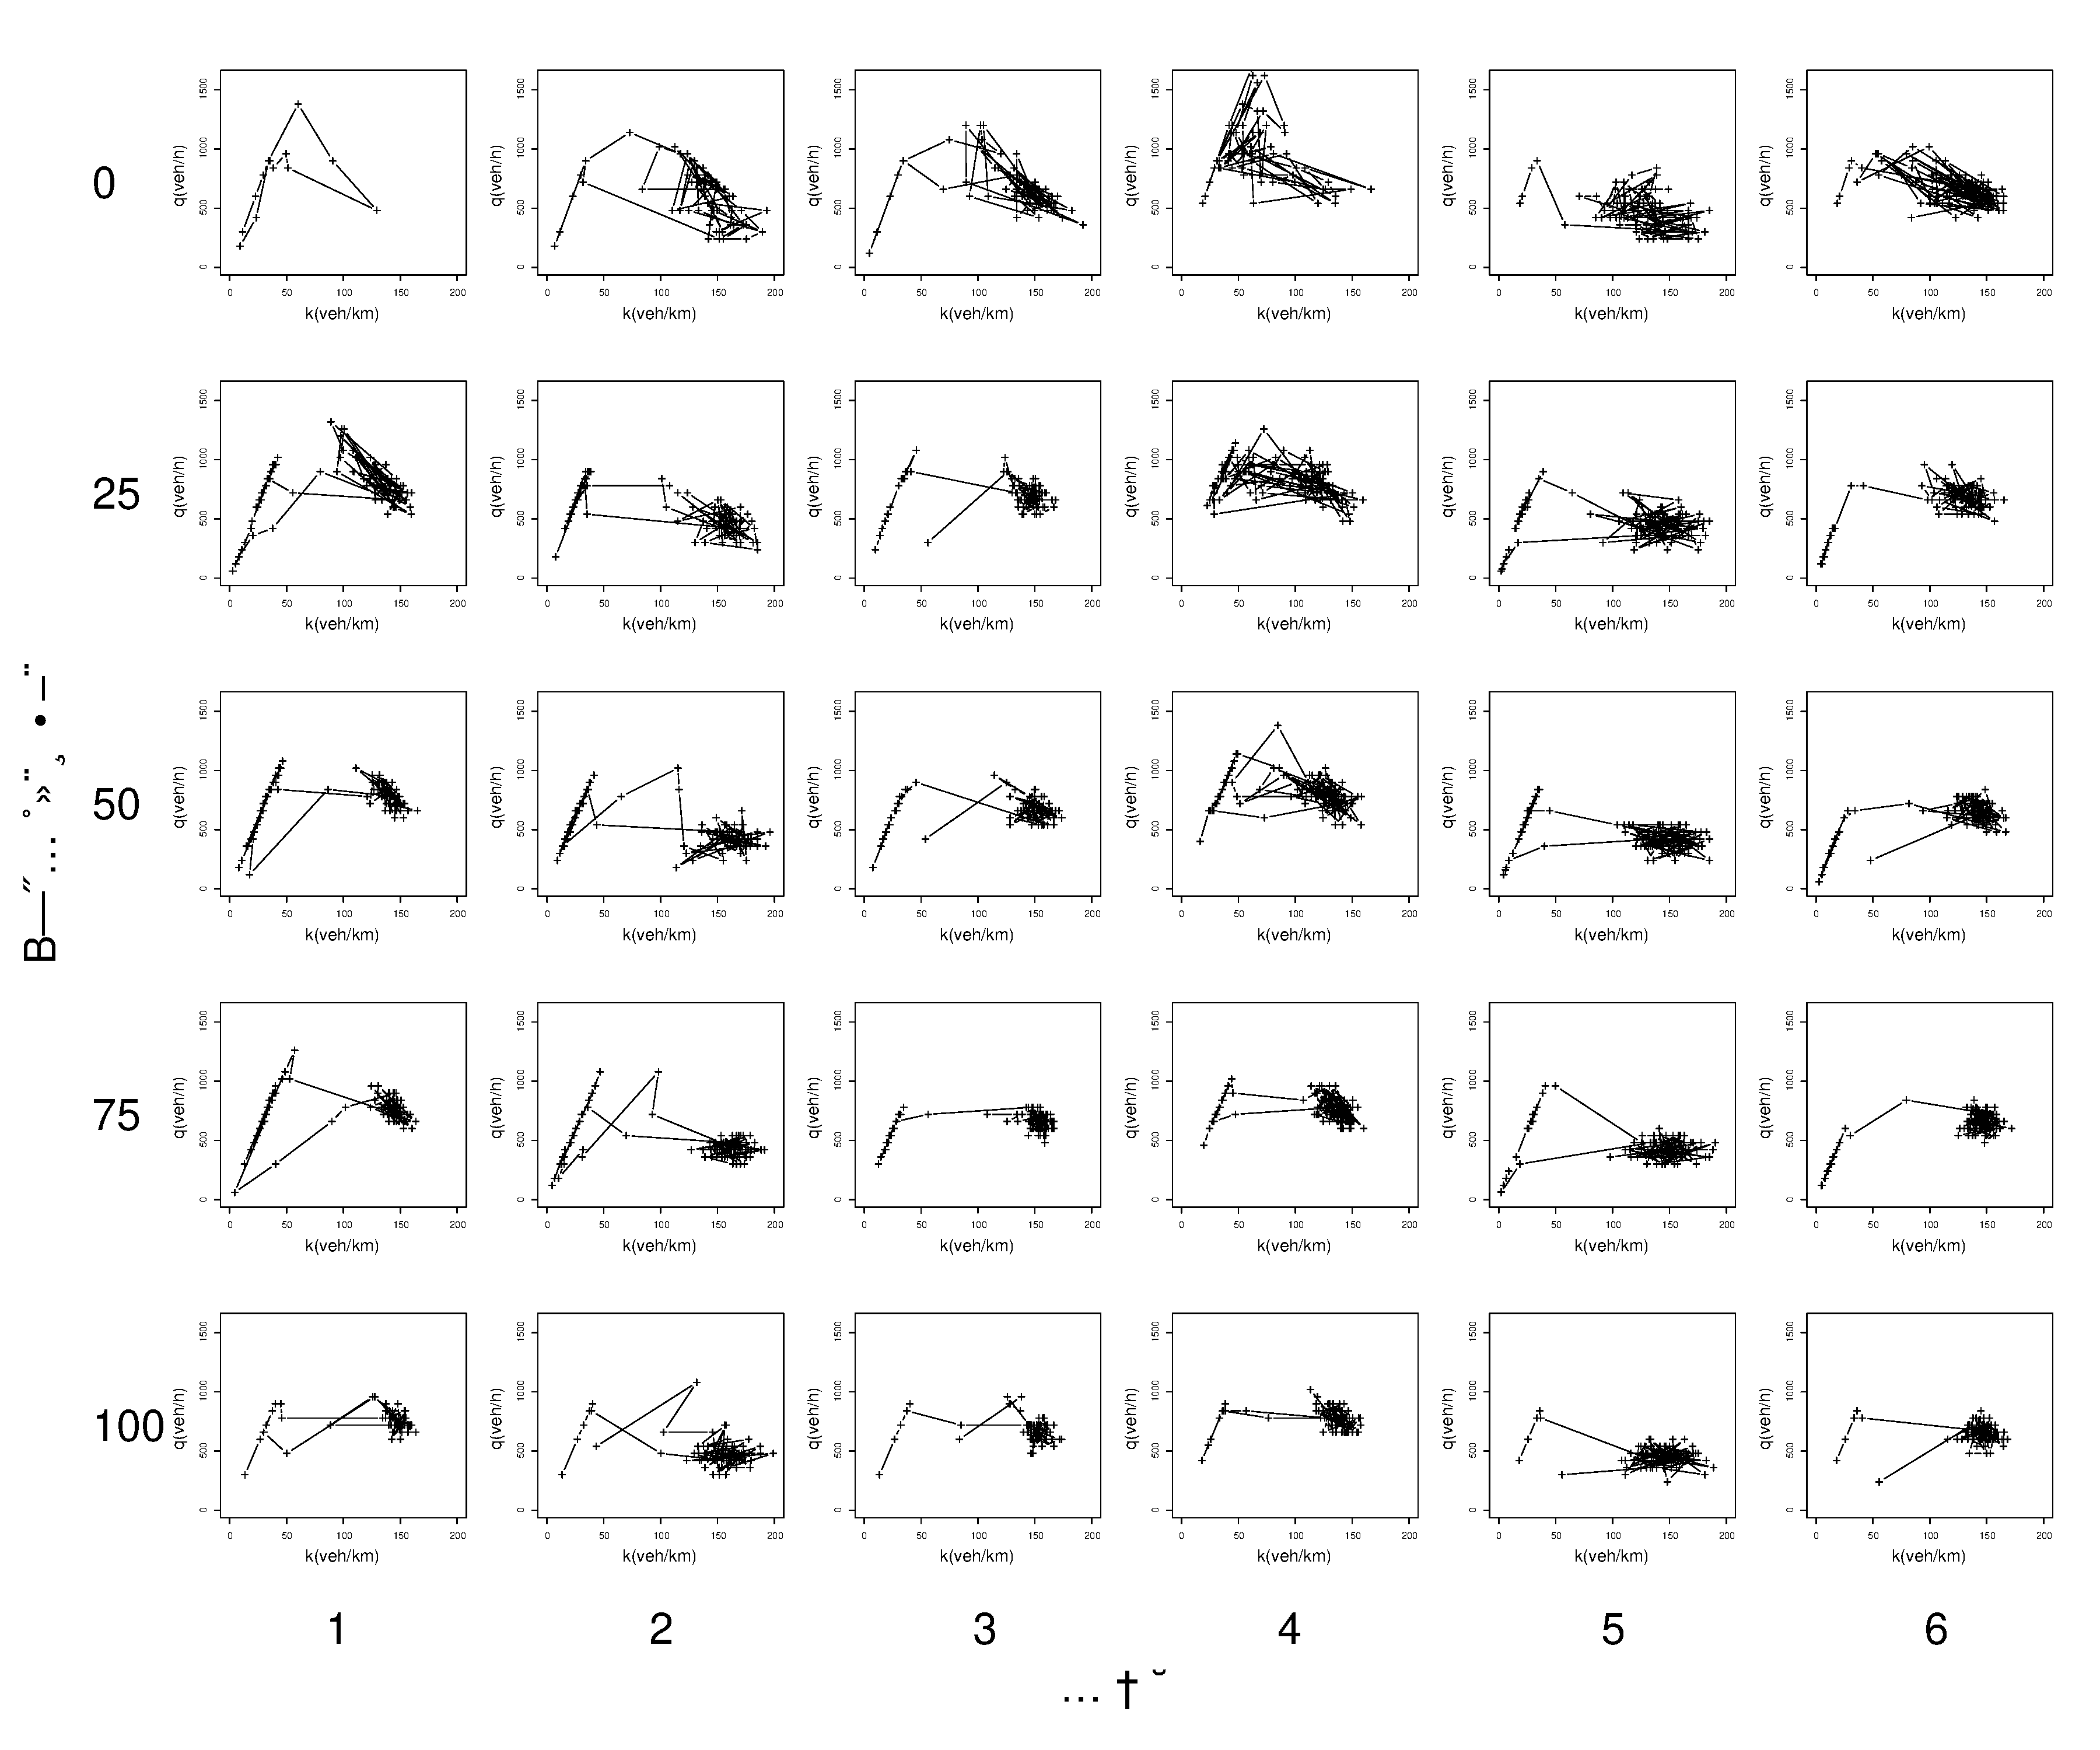
\includegraphics[width=\linewidth]{combined_kqedges}
% \caption{混合作用影响下各检测器密度流量关系图}
% \label{combined_kqedges}
% \end{center}
% \end{figure}

% \section{驾驶人行为特性对交通流安全性的影响}

% 为了评价交通流安全性,本文使用了TTC倒数的一分钟和值来评价交通流安全性,路段交通流的流量以6个检测器流量的一分钟平均值的反应。

% TTC倒数的时间平均产生密度,

% \subsection{期望速度影响因素}

% 期望速度从\autoref{factor1_ttc}流量与TTC倒数关系图看,TTC倒数的和值的绝对值最大主要出现在流量600-800之间,从图上看对其分布没有显著影响。由\autoref{factor1_box_avttc}可以看出,期望车速对,时间平均TTC倒数(或者说TTC倒数的时间产生密度)的绝对值有显著的影响,随着期望车速较高的B型驾驶人更多的混入,时间平均TTC倒数的绝对值呈现增加的趋势。当B型驾驶人的比例小于50\%时,使用不同随机数的情况差异较大,说明车辆的顺序对时间平均TTC倒数产生显著的影响。可以理解为在B型驾驶人较少时,交通流的安全性具有较大的随机性。

% \begin{figure}[!htb]%
% \centering
% \subfloat[][]{
% \label{factor1_ttc_per0}%
% 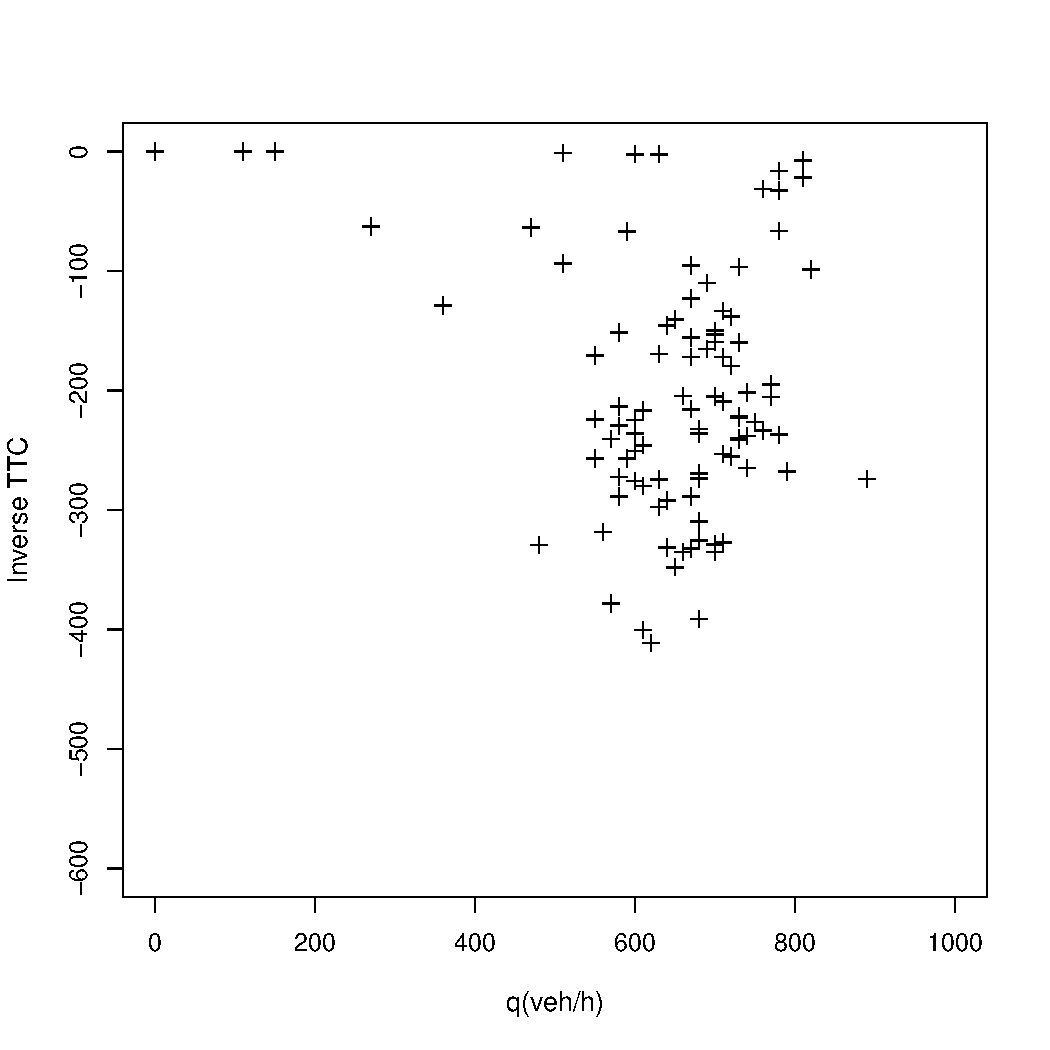
\includegraphics[width=0.25\linewidth]{factor1_ttc_per0}
% }%
% \subfloat[][]{%
% \label{factor1_ttc_per25}%
% 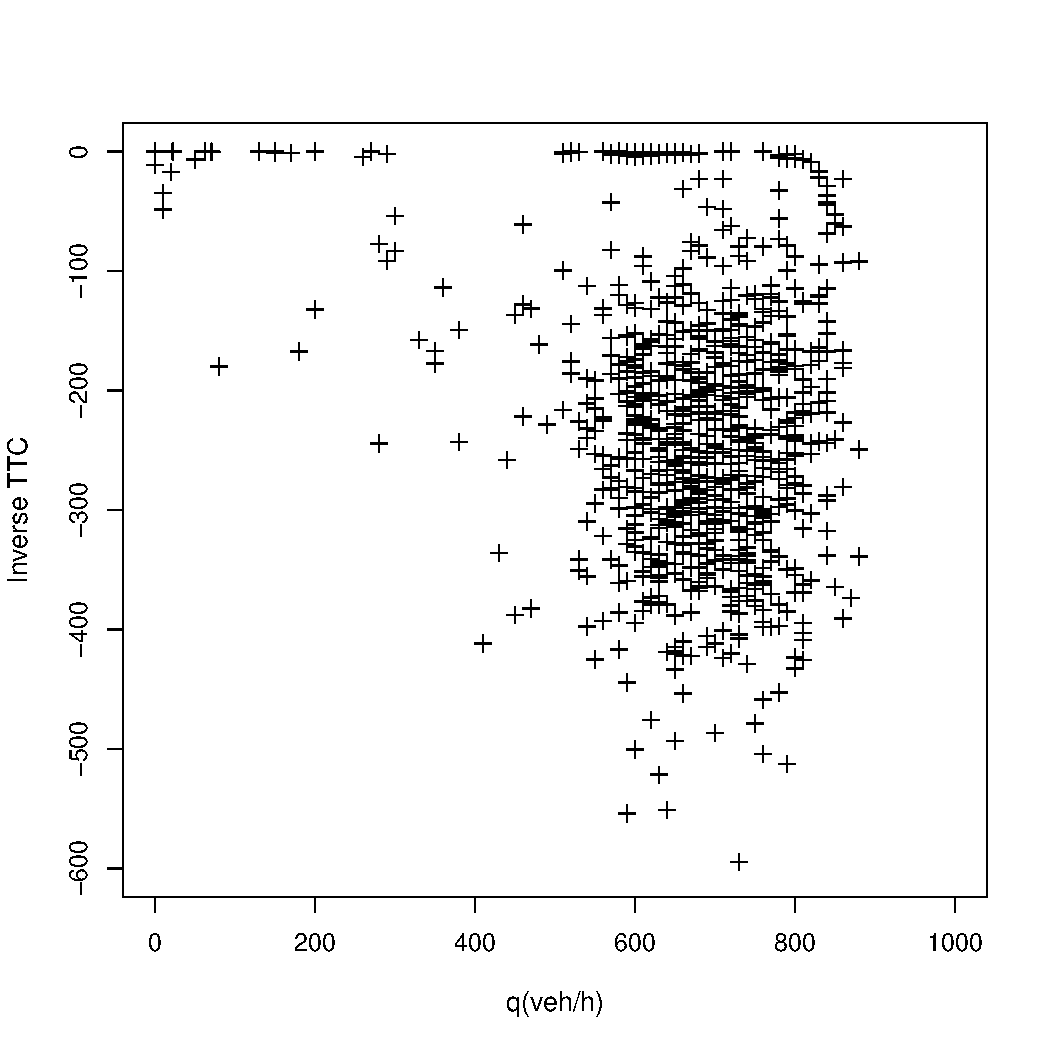
\includegraphics[width=0.25\linewidth]{factor1_ttc_per25}}
% \subfloat[][]{%
% \label{factor1_ttc_per50}%
% 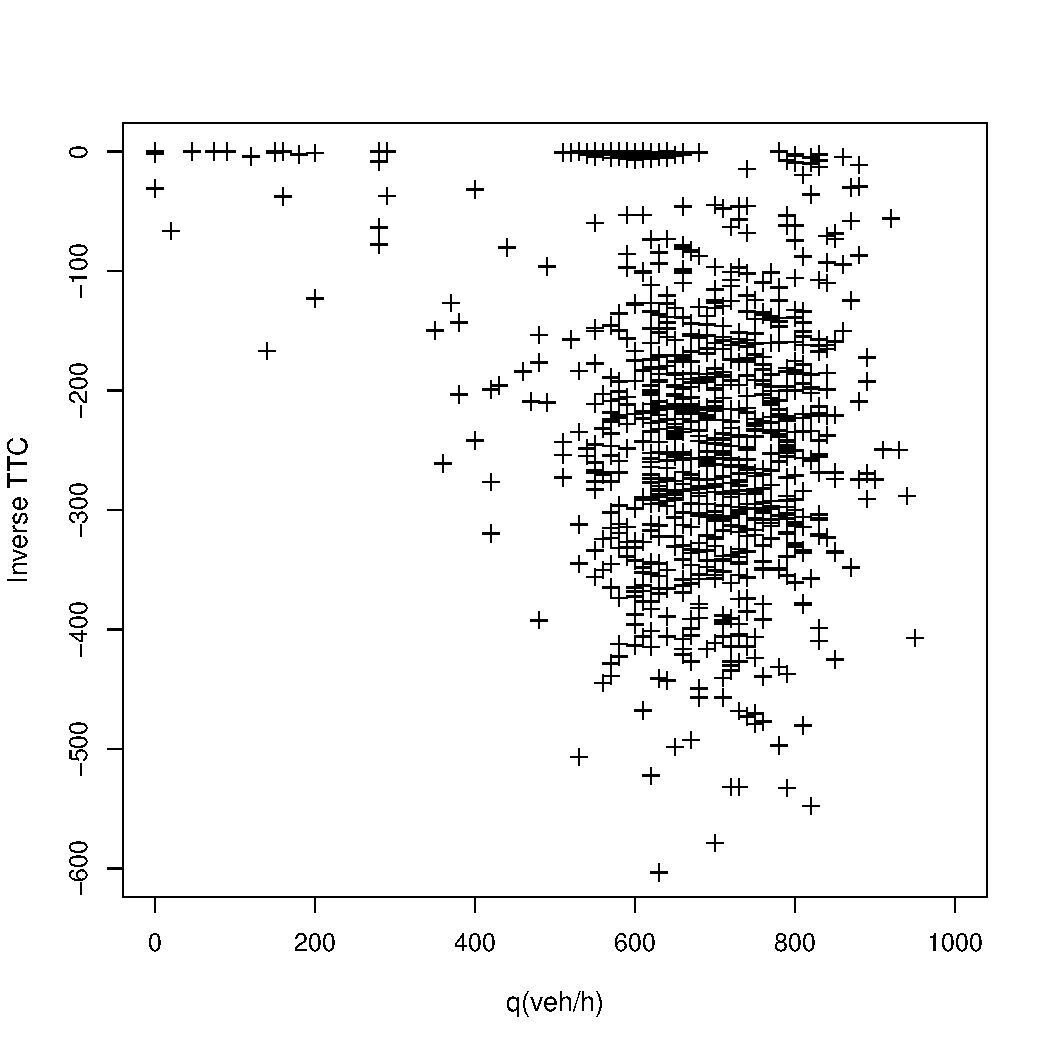
\includegraphics[width=0.25\linewidth]{factor1_ttc_per50}}\\%
% \subfloat[][]{%
% \label{factor1_ttc_per75}%
% 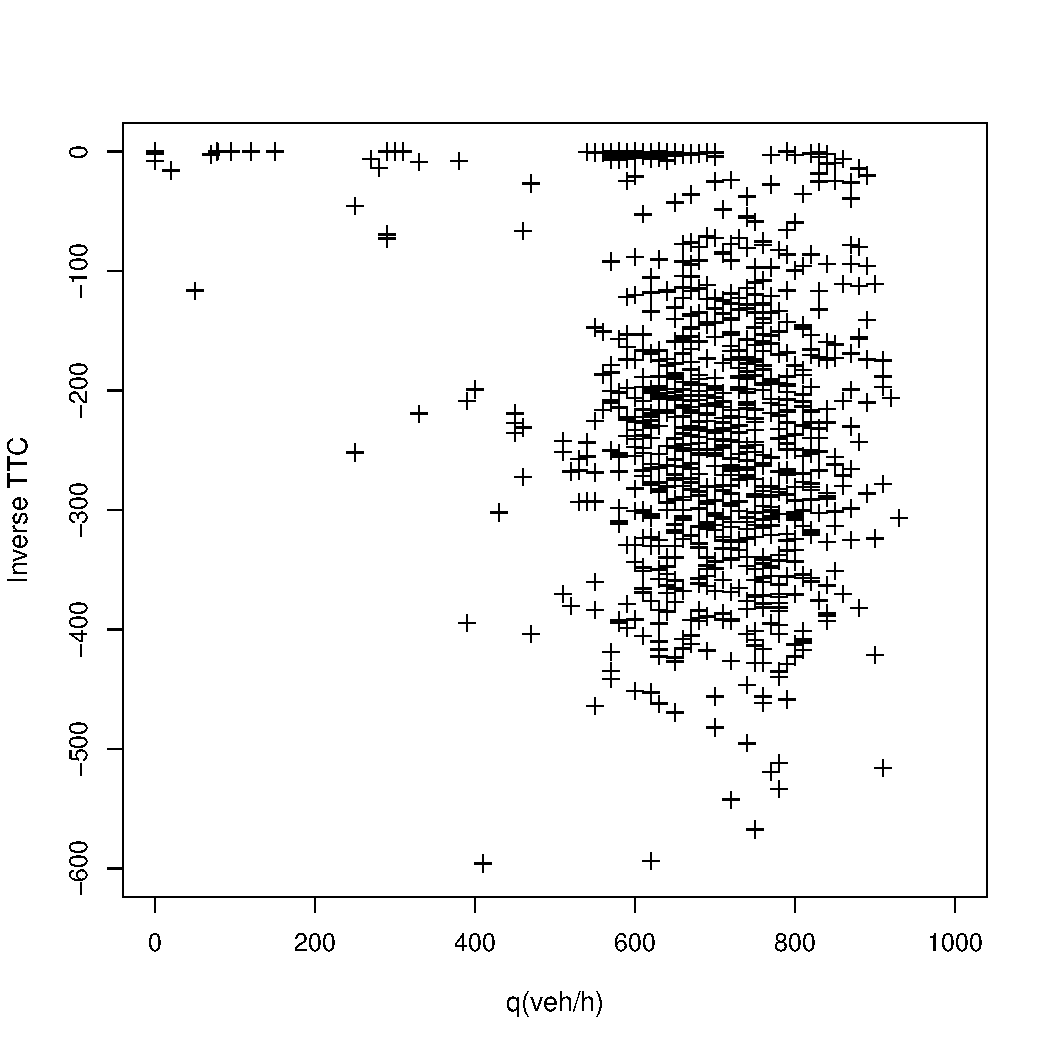
\includegraphics[width=0.25\linewidth]{factor1_ttc_per75}}%
% \subfloat[][]{%
% \label{factor1_ttc_per100}%
% 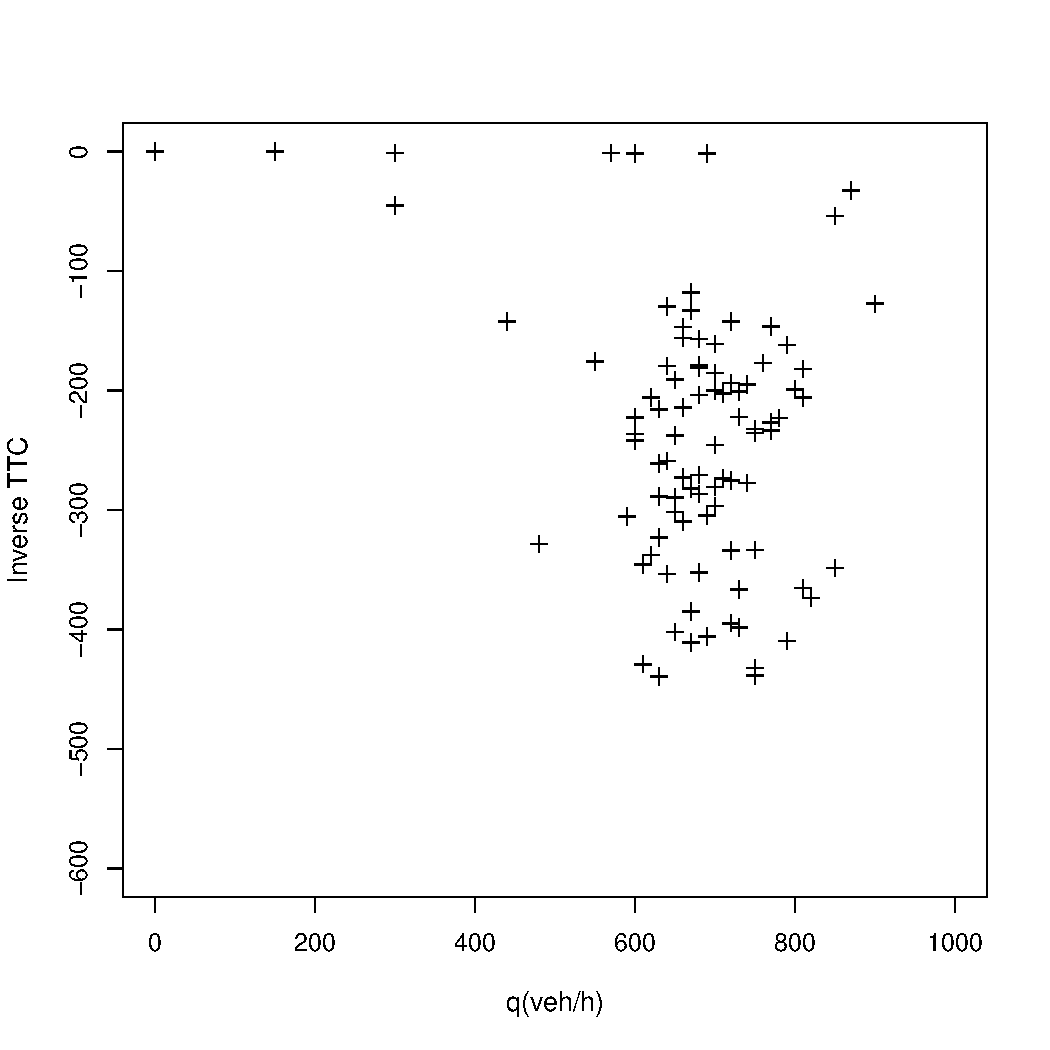
\includegraphics[width=0.25\linewidth]{factor1_ttc_per100}}
% \caption[A set of four sub-floats.]{期望速度影响下流量与TTC倒数关系图
% \subref{factor1_ttc_per0}
% \subref{factor1_ttc_per25} 
% \subref{factor1_ttc_per50}
% \subref{factor1_ttc_per75}
% \subref{factor1_ttc_per100}分别表示\autoref{speed-factor}中的B型驾驶人的百分比分别为0\%,25\%,50\%,75\%,100\%,其中流量为6个检测器平均值,TTC倒数为1分钟累计值}%
% \label{factor1_ttc}%
% \end{figure}

% \begin{figure}[!htb]
% \begin{center}
% 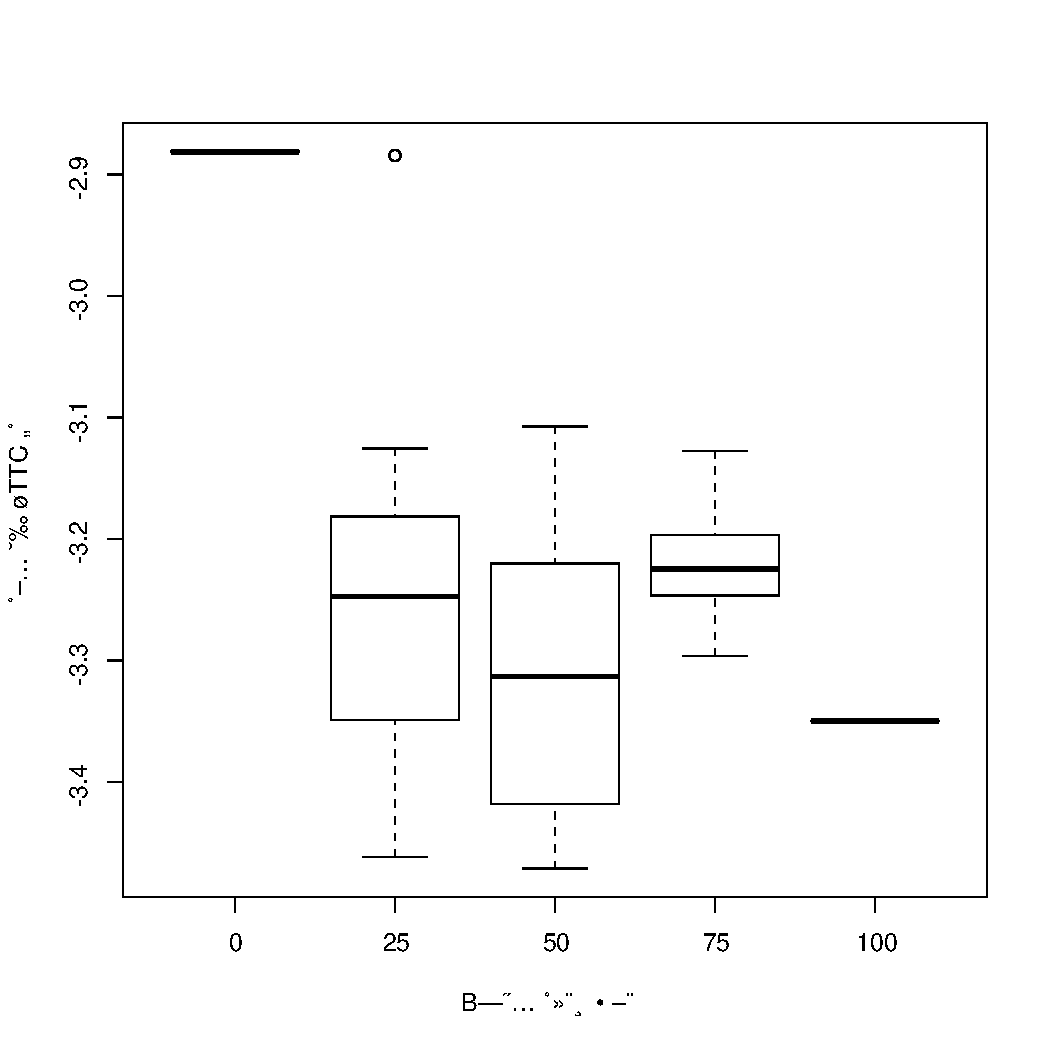
\includegraphics[width=0.7\linewidth]{factor1_box_avttc}
% \caption{期望速度影响下时间平均TTC倒数箱图}
% \label{factor1_box_avttc}
% \end{center}
% \end{figure}

% \subsection{最大减速度影响因素}

% 从\autoref{factor2_ttc}流量与TTC倒数关系图看,TTC倒数的和值的绝对值最大主要出现在流量600左右,从图上看最大减速度的变化对TTC倒数的分布没有显著影响。由\autoref{factor2_box_avttc}可以看出,期望车速对时间平均TTC倒数(或者说TTC倒数的时间产生密度)的绝对值呈现先减少后增加的趋势,随着期望车速较高的B型驾驶人更多的混入,时间平均TTC倒数的绝对值呈现先减小后增加的趋势。这似乎说明存在一个最佳的B型驾驶人混入比例使得TTC倒数的实践产生密度绝对值最小。可能的解释是,当产生速度差的扰动时,过小的减速度不利于前后车速度重新趋于同步,而过大的减速度由于驾驶人反应时间的累计作用会出现Over-Deceleration的效应。
% \begin{figure}[!htb]%
% \centering
% \subfloat[][]{
% \label{factor2_ttc_per0}%
% 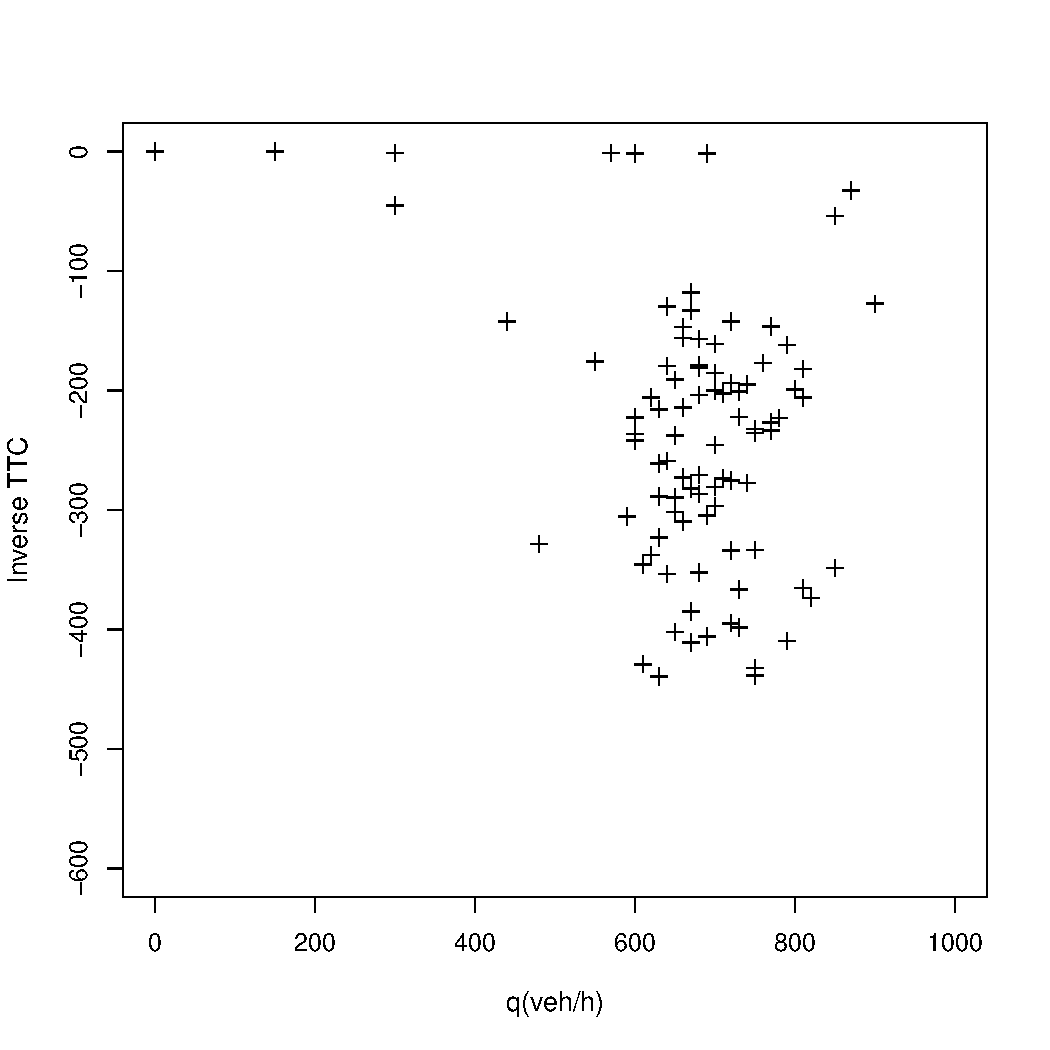
\includegraphics[width=0.25\linewidth]{factor2_ttc_per0}
% }%
% \subfloat[][]{%
% \label{factor2_ttc_per25}%
% 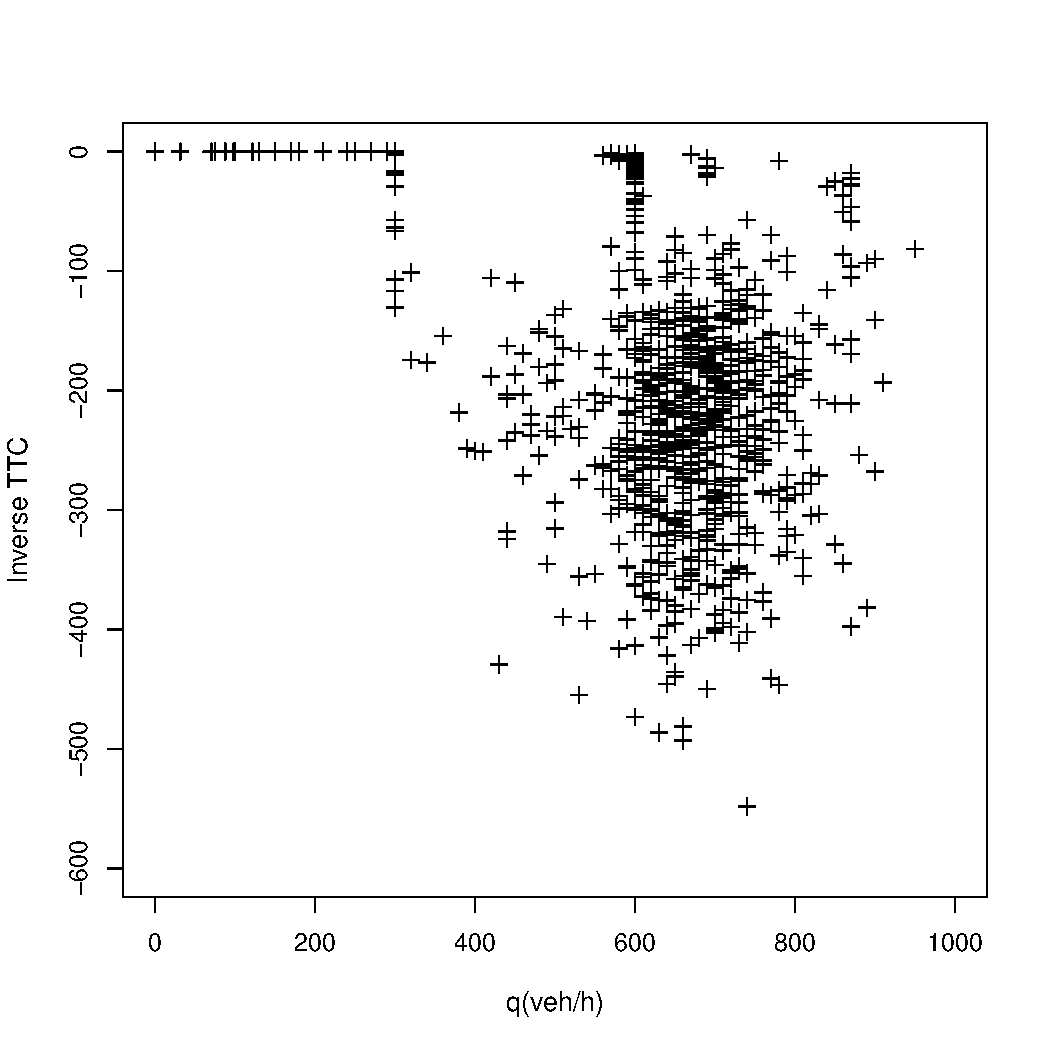
\includegraphics[width=0.25\linewidth]{factor2_ttc_per25}}
% \subfloat[][]{%
% \label{factor2_ttc_per50}%
% \includegraphics[width=0.25\linewidth]{factor2_ttc_per50}}\\%
% \subfloat[][]{%
% \label{factor2_ttc_per75}%
% \includegraphics[width=0.25\linewidth]{factor2_ttc_per75}}%
% \subfloat[][]{%
% \label{factor2_ttc_per100}%
% \includegraphics[width=0.25\linewidth]{factor2_ttc_per100}}
% \caption[A set of four sub-floats.]{最大减速度影响下流量与TTC倒数关系图
% \subref{factor2_ttc_per0}
% \subref{factor2_ttc_per25} 
% \subref{factor2_ttc_per50}
% \subref{factor2_ttc_per75}
% \subref{factor2_ttc_per100}分别表示\autoref{decel-factor}中的B型驾驶人的百分比分别为0\%,25\%,50\%,75\%,100\%,其中流量为6个检测器平均值,TTC倒数为1分钟累计值}%
% \label{factor2_ttc}%
% \end{figure}

% \begin{figure}[!htb]
% \begin{center}
% \includegraphics[width=0.7\linewidth]{factor2_box_avttc}
% \caption{最大减速度影响下时间平均TTC倒数箱图}
% \label{factor2_box_avttc}
% \end{center}
% \end{figure}

% \subsection{混合影响因素}

% 从\autoref{combined_ttc}流量与TTC倒数关系图看,混合影响因素作用下,随着B型驾驶人(代表专业驾驶人)的增加,相同流量下TTC倒数的绝对值的最大值有增加的趋势,意味着交通流偏向不安全的方向。而混合作用影响下的时间平均倒数结果与最大减速影响的结果相似,这仍表明似乎最大减速度是交通流的主要影响因素。
% \begin{figure}[!htb]%
% \centering
% \subfloat[][]{
% \label{combined_ttc_per0}%
% \includegraphics[width=0.25\linewidth]{combined_ttc_per0}
% }%
% \subfloat[][]{%
% \label{combined_ttc_per25}%
% \includegraphics[width=0.25\linewidth]{combined_ttc_per25}}
% \subfloat[][]{%
% \label{combined_ttc_per50}%
% \includegraphics[width=0.25\linewidth]{combined_ttc_per50}}\\%
% \subfloat[][]{%
% \label{combined_ttc_per75}%
% \includegraphics[width=0.25\linewidth]{combined_ttc_per75}}%
% \subfloat[][]{%
% \label{combined_ttc_per100}%
% \includegraphics[width=0.25\linewidth]{combined_ttc_per100}}
% \caption[A set of four sub-floats.]{混合作用影响下流量与TTC倒数关系图
% \subref{combined_ttc_per0}
% \subref{combined_ttc_per25} 
% \subref{combined_ttc_per50}
% \subref{combined_ttc_per75}
% \subref{combined_ttc_per100}分别表示\autoref{combined-factor}中的B型驾驶人的百分比分别为0\%,25\%,50\%,75\%,100\%,其中流量为6个检测器平均值,TTC倒数为1分钟累计值}%
% \label{combined_ttc}%
% \end{figure}

% \begin{figure}[!htb]
% \begin{center}
% \includegraphics[width=0.7\linewidth]{combined_box_avttc}
% \caption{混合作用影响下时间平均TTC倒数箱图}
% \label{combined_box_avttc}
% \end{center}
% \end{figure}

% \section{本章小结}
% 本章通过微观交通流模拟仿真研究了驾驶人行为特性对交通流的影响。根据第四章驾驶人行为参数的差异性结果,分别构造了不同期望速度,最大减速度以及两参数组合的不同驾驶人,以不同比例混合进行模拟,结果表明,期望车速及最大减速度对交通流的效率性及安全性存在不同特点和程度的影响,而主要的影响因素是驾驶人的最大减速度。

\section{驾驶人行为特性对交通流效率性的影响}

    \renewcommand{\topfraction}{0.9}	% max fraction of floats at top
    \renewcommand{\bottomfraction}{0.8}	% max fraction of floats at bottom
    %   Parameters for TEXT pages (not float pages):
    \setcounter{topnumber}{2}
    \setcounter{bottomnumber}{2}
    \setcounter{totalnumber}{4}     % 2 may work better
    \setcounter{dbltopnumber}{2}    % for 2-column pages
    \renewcommand{\dbltopfraction}{0.9}	% fit big float above 2-col. text
    \renewcommand{\textfraction}{0.00}	% allow minimal text w. figs
    %   Parameters for FLOAT pages (not text pages):
    \renewcommand{\floatpagefraction}{0.7}	% require fuller float pages
	% N.B.: floatpagefraction MUST be less than topfraction !!
    \renewcommand{\dblfloatpagefraction}{0.7}	% require fuller float pages



\subsection{期望速度影响因素}
%根据\autoref{speed-factor}的驾驶人参数进行混合模拟,得到:
\autoref{factor1_box_ttime}给出了期望速度影响下模拟总用时的变化箱图,随着\autoref{speed-factor}中期望速度较大的B型驾驶人的增加,模拟所用时间呈现下降的趋势。对于单纯类型的驾驶人组合,期望速度由6.48m/s(23.3km/h)增加8.09m/s(30.6km/h),增加24.8\%,模拟用时从6720s下降到6540s,降低了3\%。当不同类型驾驶人混合驶入时模拟时间在一定的范围内变化,例如当有75\%的B型驾驶人混入时,模拟时间的变动范围超过了200s,这表明车辆的驶入顺序对模拟时间产生影响,不同期望速度驾驶人的混合增加了交通流的随机性。

\autoref{factor1_vq}给出了期望速度影响下速度流量关系的变化情况,由\autoref{factor1_vq}可以看出,期望速度主要对速度-流量关系图中的形状有影响,对最大通行能力和最大通行能力所对应的最佳车速基本没有影响,图中可以看出最大通行能力约为1600veh/h,最佳速度均大约在22km/h。期望速度对速度-流量关系图中的形状的影响主要体现在最佳车速的右侧的自由流的阶段。由于两组的期望速度均超过了最佳车速,因此不能排除当期望速度低于最佳车速时可能会对最大通行能力产生影响。


\autoref{factor1_kq}给出了期望速度影响下密度流量关系的变化情况,由\autoref{factor1_kq}可以看出期望速度对最佳密度基本没有影响,最佳密度大约为75veh/km。根据Kerner的三相交通流理论,道路介于最大和最小通行能力之间具有无数个通行能力,\autoref{factor1_kq}中a、b、c、d的最小通行能力大约为500veh/h,而e的最小通行能力稍大于其他的情况,这似乎表明最小通行能力受到驾驶人群体中最低期望车速的影响。

\begin{figure}[htb]
\begin{center}
\includegraphics[width=0.5\linewidth]{factor1_box_ttime}
\caption{期望速度影响下模拟用时箱图}
\label{factor1_box_ttime}
\end{center}
\end{figure}


\begin{figure}[htb]%
\centering
\subfloat[][]{
\label{factor1_vq_per0}%
\includegraphics[width=0.25\linewidth]{factor1_vq_per0}
}%
\subfloat[][]{%
\label{factor1_vq_per25}%
\includegraphics[width=0.25\linewidth]{factor1_vq_per25}}
\subfloat[][]{%
\label{factor1_vq_per50}%
\includegraphics[width=0.25\linewidth]{factor1_vq_per50}}\\%
\subfloat[][]{%
\label{factor1_vq_per75}%
\includegraphics[width=0.25\linewidth]{factor1_vq_per75}}%
\subfloat[][]{%
\label{factor1_vq_per100}%
\includegraphics[width=0.25\linewidth]{factor1_vq_per100}}
\caption[A set of four sub-floats.]{期望速度影响下速度流量关系图
\subref{factor1_vq_per0}
\subref{factor1_vq_per25} 
\subref{factor1_vq_per50}
\subref{factor1_vq_per75}
\subref{factor1_vq_per100}分别表示\autoref{speed-factor}中的B型驾驶人的百分比分别为0\%,25\%,50\%,75\%,100\%}%
\label{factor1_vq}%
\end{figure}


\begin{figure}[htb]%
\centering
\subfloat[][]{
\label{factor1_kq_per0}%
\includegraphics[width=0.25\linewidth]{factor1_kq_per0}
}%
\subfloat[][]{%
\label{factor1_kq_per25}%
\includegraphics[width=0.25\linewidth]{factor1_kq_per25}}
\subfloat[][]{%
\label{factor1_kq_per50}%
\includegraphics[width=0.25\linewidth]{factor1_kq_per50}}\\%
\subfloat[][]{%
\label{factor1_kq_per75}%
\includegraphics[width=0.25\linewidth]{factor1_kq_per75}}%
\subfloat[][]{%
\label{factor1_kq_per100}%
\includegraphics[width=0.25\linewidth]{factor1_kq_per100}}
\caption[A set of four sub-floats.]{期望速度影响下的密度流量关系图
\subref{factor1_kq_per0}
\subref{factor1_kq_per25} 
\subref{factor1_kq_per50}
\subref{factor1_kq_per75}
\subref{factor1_kq_per100}分别表示\autoref{speed-factor}中的B型驾驶人的百分比分别为0\%,25\%,50\%,75\%,100\%}%
\label{factor1_kq}%
\end{figure}

\FloatBarrier



%由于低期望车速的驾驶人的存在,???根据三相交通流中Speed adaptation效用的作用,低速车辆的阻碍造成最低通行能力的下降是可以理解的。

\subsection{最大减速度影响因素}



\autoref{factor2_box_ttime}给出了最大减速度影响下模拟总用时的变化箱图,随着\autoref{decel-factor}中最大减速度较大的B型驾驶人的增加,模拟所用时间呈现上升的趋势。对于单纯类型的驾驶人组合,最大减速度由2.33$m/s^2$增加4.29$m/s^2$,增加84\%,模拟用时从6540s增加到7080s,增加了8.3\%。少量的B型驾驶人即可对总模拟用时造成较大影响,并且使得模拟时间具有很大随机性。

\autoref{factor2_vq}和\autoref{factor2_kq}分别给出了最大减速度影响下速度流量关系图和最大减速度影响下的密度流量关系图,可以看出,随着\autoref{decel-factor}中最大减速度较大的B型驾驶人的比例增加,在速度流量和密度流量关系图上均更难达到最大通行能力。这种趋势随着B型驾驶人的增加而更为明显。最大减速度的增加造成密度流量图上,集中在J线以上,相对不稳定的状态。\autoref{factor2_kqedges}给出了最大减速度影响下各检测器密度流量关系图,从各检测器的密度流量状态跃迁图看,最为明显的是,检测器1和4的最大或接近最大通行能力,随着B型驾驶人的更多的混入,从自由流的状态更多的往同步流状态跃迁。这表明最大减速度的增加对交通流的效率性存在负面的影响。

\begin{figure}[htb]
\begin{center}
\includegraphics[width=0.5\linewidth]{factor2_box_ttime}
\caption{最大减速度影响下模拟用时箱图}
\label{factor2_box_ttime}
\end{center}
\end{figure}

\begin{figure}[htb]%
\centering
\subfloat[][]{
\label{factor2_vq_per0}%
\includegraphics[width=0.25\linewidth]{factor2_vq_per0}
}%
\subfloat[][]{%
\label{factor2_vq_per25}%
\includegraphics[width=0.25\linewidth]{factor2_vq_per25}}
\subfloat[][]{%
\label{factor2_vq_per50}%
\includegraphics[width=0.25\linewidth]{factor2_vq_per50}}\\%
\subfloat[][]{%
\label{factor2_vq_per75}%
\includegraphics[width=0.25\linewidth]{factor2_vq_per75}}%
\subfloat[][]{%
\label{factor2_vq_per100}%
\includegraphics[width=0.25\linewidth]{factor2_vq_per100}}
\caption[A set of four sub-floats.]{最大减速度影响下速度流量关系图
\subref{factor2_vq_per0}
\subref{factor2_vq_per25} 
\subref{factor2_vq_per50}
\subref{factor2_vq_per75}
\subref{factor2_vq_per100}分别表示\autoref{decel-factor}中的B型驾驶人的百分比分别为0\%,25\%,50\%,75\%,100\%}%
\label{factor2_vq}%
\end{figure}



\begin{figure}[htb]%
\centering
\subfloat[][]{
\label{factor2_kq_per0}%
\includegraphics[width=0.25\linewidth]{factor2_kq_per0}
}%
\subfloat[][]{%
\label{factor2_kq_per25}%
\includegraphics[width=0.25\linewidth]{factor2_kq_per25}}
\subfloat[][]{%
\label{factor2_kq_per50}%
\includegraphics[width=0.25\linewidth]{factor2_kq_per50}}\\%
\subfloat[][]{%
\label{factor2_kq_per75}%
\includegraphics[width=0.25\linewidth]{factor2_kq_per75}}%
\subfloat[][]{%
\label{factor2_kq_per100}%
\includegraphics[width=0.25\linewidth]{factor2_kq_per100}}
\caption[A set of four sub-floats.]{最大减速度影响下的密度流量关系图
\subref{factor2_kq_per0}
\subref{factor2_kq_per25} 
\subref{factor2_kq_per50}
\subref{factor2_kq_per75}
\subref{factor2_kq_per100}分别表示\autoref{decel-factor}中的B型驾驶人的百分比分别为0\%,25\%,50\%,75\%,100\%}%
\label{factor2_kq}%
\end{figure}




\begin{figure}[htb]
\begin{center}
\includegraphics[width=\linewidth]{factor2_kqedges}
\caption{最大减速度影响下各检测器密度流量关系图}
\label{factor2_kqedges}
\end{center}
\end{figure}

\FloatBarrier

\subsection{混合影响因素}

\autoref{combined_box_ttime}、\autoref{combined_vq}、\autoref{combined_kq}、\autoref{combined_kqedges},分别给出了混合作用影响下模拟用时箱图、速度流量关系图、密度流量关系图和各检测器密度流量关系图。其结果与最大减速度影响下的结果相似,可以推断对交通流效率性的影响,主要的贡献成分来自于最大减速度的影响,最大减速度越大则交通流越难达到最大通行能力,也越多的处于较为不稳定的同步流状态。

\begin{figure}[htb]
\begin{center}
\includegraphics[width=0.5\linewidth]{combined_box_ttime}
\caption{混合作用影响下模拟用时箱图}
\label{combined_box_ttime}
\end{center}
\end{figure}



\begin{figure}[htb]%
\centering
\subfloat[][]{
\label{combined_vq_per0}%
\includegraphics[width=0.25\linewidth]{combined_vq_per0}
}%
\subfloat[][]{%
\label{combined_vq_per25}%
\includegraphics[width=0.25\linewidth]{combined_vq_per25}}
\subfloat[][]{%
\label{combined_vq_per50}%
\includegraphics[width=0.25\linewidth]{combined_vq_per50}}\\%
\subfloat[][]{%
\label{combined_vq_per75}%
\includegraphics[width=0.25\linewidth]{combined_vq_per75}}%
\subfloat[][]{%
\label{combined_vq_per100}%
\includegraphics[width=0.25\linewidth]{combined_vq_per100}}
\caption[A set of four sub-floats.]{混合作用影响下速度流量关系图
\subref{combined_vq_per0}
\subref{combined_vq_per25} 
\subref{combined_vq_per50}
\subref{combined_vq_per75}
\subref{combined_vq_per100}分别表示\autoref{combined-factor}中的B型驾驶人的百分比分别为0\%,25\%,50\%,75\%,100\%}%
\label{combined_vq}%
\end{figure}


\begin{figure}[htb]%
\centering
\subfloat[][]{
\label{combined_kq_per0}%
\includegraphics[width=0.25\linewidth]{combined_kq_per0}
}%
\subfloat[][]{%
\label{combined_kq_per25}%
\includegraphics[width=0.25\linewidth]{combined_kq_per25}}
\subfloat[][]{%
\label{combined_kq_per50}%
\includegraphics[width=0.25\linewidth]{combined_kq_per50}}\\%
\subfloat[][]{%
\label{combined_kq_per75}%
\includegraphics[width=0.25\linewidth]{combined_kq_per75}}%
\subfloat[][]{%
\label{combined_kq_per100}%
\includegraphics[width=0.25\linewidth]{combined_kq_per100}}
\caption[A set of four sub-floats.]{混合作用影响下的密度流量关系图
\subref{combined_kq_per0}
\subref{combined_kq_per25} 
\subref{combined_kq_per50}
\subref{combined_kq_per75}
\subref{combined_kq_per100}分别表示\autoref{combined-factor}中的B型驾驶人的百分比分别为0\%,25\%,50\%,75\%,100\%}%
\label{combined_kq}%
\end{figure}

\begin{figure}[htb]
\begin{center}
\includegraphics[width=\linewidth]{combined_kqedges}
\caption{混合作用影响下各检测器密度流量关系图}
\label{combined_kqedges}
\end{center}
\end{figure}

\FloatBarrier

\section{驾驶人行为特性对交通流安全性的影响}

为了评价交通流安全性,本文使用了TTC倒数的一分钟和值以及TTC倒数的时间平均产生密度来评价交通流安全性,路段交通流的流量以6个检测器流量的一分钟平均值来代表。


\subsection{期望速度影响因素}

\autoref{factor1_ttc}给出了期望速度影响下流量与TTC倒数关系变化情况,可以看出TTC倒数的和值的绝对值最大出现在流量600-800之间,从图上看期望速度对TTC倒数和值的分布没有显著影响。\autoref{factor1_box_avttc}给出了期望速度影响下流量与时间平均TTC倒数关系变化箱图,可以看出期望车速对时间平均TTC倒数(TTC倒数的时间产生密度)的绝对值有显著的影响,随着期望车速较高的B型驾驶人的混入,时间平均TTC倒数的绝对值呈现增加的趋势,对于单纯类型的驾驶人组合,期望速度由6.48m/s(23.3km/h)增加8.09m/s(30.6km/h),增加24.8\%,时间平均TTC倒数的绝对值从2.88增加到3.35,增加了16.3\%。这表明期望速度的增加对交通流的安全性产生负面的影响。当B型驾驶人的比例小于50\%时,使用不同随机数的情况差异较大,说明车辆的顺序对时间平均TTC倒数产生显著的影响。可以理解为在B型驾驶人少于A型驾驶人时时,交通流的安全性具有较大的随机性。

\begin{figure}[htb]%
\centering
\subfloat[][]{
\label{factor1_ttc_per0}%
\includegraphics[width=0.25\linewidth]{factor1_ttc_per0}
}%
\subfloat[][]{%
\label{factor1_ttc_per25}%
\includegraphics[width=0.25\linewidth]{factor1_ttc_per25}}
\subfloat[][]{%
\label{factor1_ttc_per50}%
\includegraphics[width=0.25\linewidth]{factor1_ttc_per50}}\\%
\subfloat[][]{%
\label{factor1_ttc_per75}%
\includegraphics[width=0.25\linewidth]{factor1_ttc_per75}}%
\subfloat[][]{%
\label{factor1_ttc_per100}%
\includegraphics[width=0.25\linewidth]{factor1_ttc_per100}}
\caption[A set of four sub-floats.]{期望速度影响下流量与TTC倒数关系图
\subref{factor1_ttc_per0}
\subref{factor1_ttc_per25} 
\subref{factor1_ttc_per50}
\subref{factor1_ttc_per75}
\subref{factor1_ttc_per100}分别表示\autoref{speed-factor}中的B型驾驶人的百分比分别为0\%,25\%,50\%,75\%,100\%,其中流量为6个检测器平均值,TTC倒数为1分钟累计值}%
\label{factor1_ttc}%
\end{figure}

\begin{figure}[htb]
\begin{center}
\includegraphics[width=0.5\linewidth]{factor1_box_avttc}
\caption{期望速度影响下时间平均TTC倒数箱图}
\label{factor1_box_avttc}
\end{center}
\end{figure}

\FloatBarrier

\subsection{最大减速度影响因素}

\autoref{factor2_ttc}给出了最大减速度影响下的流量与TTC倒数和值关系图,图中TTC倒数的和值的绝对值最大主要出现在流量600左右,从图上看最大减速度的变化对TTC倒数的分布没有显著影响。\autoref{factor2_box_avttc}给出了最大减速度影响下流量与时间平均TTC倒数关系变化箱图,可以看出随着最大减速度较高的B型驾驶人更多的混入,时间平均TTC倒数的绝对值呈现先减小后增加的趋势。这似乎说明存在一个最佳的B型驾驶人混入比例使得TTC倒数的实践产生密度绝对值最小。可能的解释是,当产生速度差的扰动时,过小的减速度不利于前后车速度重新趋于同步,而过大的减速度由于驾驶人反应时间对减速程度的累计作用会增强Over-Deceleration效应,从而导致速度扰动的增加。
\begin{figure}[htb]%
\centering
\subfloat[][]{
\label{factor2_ttc_per0}%
\includegraphics[width=0.25\linewidth]{factor2_ttc_per0}
}%
\subfloat[][]{%
\label{factor2_ttc_per25}%
\includegraphics[width=0.25\linewidth]{factor2_ttc_per25}}
\subfloat[][]{%
\label{factor2_ttc_per50}%
\includegraphics[width=0.25\linewidth]{factor2_ttc_per50}}\\%
\subfloat[][]{%
\label{factor2_ttc_per75}%
\includegraphics[width=0.25\linewidth]{factor2_ttc_per75}}%
\subfloat[][]{%
\label{factor2_ttc_per100}%
\includegraphics[width=0.25\linewidth]{factor2_ttc_per100}}
\caption[A set of four sub-floats.]{最大减速度影响下流量与TTC倒数关系图
\subref{factor2_ttc_per0}
\subref{factor2_ttc_per25} 
\subref{factor2_ttc_per50}
\subref{factor2_ttc_per75}
\subref{factor2_ttc_per100}分别表示\autoref{decel-factor}中的B型驾驶人的百分比分别为0\%,25\%,50\%,75\%,100\%,其中流量为6个检测器平均值,TTC倒数为1分钟累计值}%
\label{factor2_ttc}%
\end{figure}

\begin{figure}[htb]
\begin{center}
\includegraphics[width=0.5\linewidth]{factor2_box_avttc}
\caption{最大减速度影响下时间平均TTC倒数箱图}
\label{factor2_box_avttc}
\end{center}
\end{figure}

\FloatBarrier

\subsection{混合影响因素}

\autoref{combined_ttc}给出了混合影响因素影响下流量与TTC倒数和值关系的变化情况,从\autoref{combined_ttc}中可以看出随着B型驾驶人(代表专业驾驶人)的增加,相同流量下TTC倒数和值的绝对值的最大值有增加的趋势,意味着交通流偏向不安全的方向。\autoref{combined_box_avttc}给出了混合影响因素作用下流量与时间平均TTC倒数关系变化箱图,混合作用影响下的TTC时间平均倒数结果与最大减速影响的结果相似,这仍表明最大减速度是交通流的主要影响因素。
\begin{figure}[htb]%
\centering
\subfloat[][]{
\label{combined_ttc_per0}%
\includegraphics[width=0.25\linewidth]{combined_ttc_per0}
}%
\subfloat[][]{%
\label{combined_ttc_per25}%
\includegraphics[width=0.25\linewidth]{combined_ttc_per25}}
\subfloat[][]{%
\label{combined_ttc_per50}%
\includegraphics[width=0.25\linewidth]{combined_ttc_per50}}\\%
\subfloat[][]{%
\label{combined_ttc_per75}%
\includegraphics[width=0.25\linewidth]{combined_ttc_per75}}%
\subfloat[][]{%
\label{combined_ttc_per100}%
\includegraphics[width=0.25\linewidth]{combined_ttc_per100}}
\caption[A set of four sub-floats.]{混合作用影响下流量与TTC倒数关系图
\subref{combined_ttc_per0}
\subref{combined_ttc_per25} 
\subref{combined_ttc_per50}
\subref{combined_ttc_per75}
\subref{combined_ttc_per100}分别表示\autoref{combined-factor}中的B型驾驶人的百分比分别为0\%,25\%,50\%,75\%,100\%,其中流量为6个检测器平均值,TTC倒数为1分钟累计值}%
\label{combined_ttc}%
\end{figure}

\begin{figure}[htb]
\begin{center}
\includegraphics[width=0.5\linewidth]{combined_box_avttc}
\caption{混合作用影响下时间平均TTC倒数箱图}
\label{combined_box_avttc}
\end{center}
\end{figure}

\FloatBarrier

\section{本章小结}
本章通过微观交通流模拟仿真研究了驾驶人行为特性对交通流的影响。根据第四章驾驶人行为参数的差异性结果,分别构造了不同期望速度,最大减速度以及两参数组合的不同驾驶人,以不同比例混合进行模拟,结果表明,期望车速及最大减速度对交通流的效率性及安全性存在不同特点和程度的影响,而主要的影响因素是驾驶人的最大减速度。
